\documentclass[Thesis.tex]{subfiles}
\begin{document}
\chapter{Quantum Dots}
\label{chp:quantum-dots}

We now present results for all methods discussed, applied on the example system
of Quantum Dots (QD) from \cref{sec:quantum-dots-theory}. We present first some
benchmarks using a typical Slater-Jastrow wave function form, followed by
introduction of neural network-based wave functions.

\section{Benchmark}

As we shall restrict this analysis to only two interacting particles in the QD,
$\vX = (\vx_1\ \vx_2)$, our benchmark wave function is simple. We build
it up using the product of single particle ground states (Gaussian), multiplied
by a Pade-Jastrow correlation term:\footnote{We drop the constant factor from~\cref{eq:Phi-non-inter} because we have not normalized the wave function.}

\begin{align}
  \label{eq:qd-pade-jastrow-anzats}
  \psi_{PJ}(\vX) &= \Phi(\vX) \,J_P(\vX)\\
  &= \exp(-\alpha_G\sum_{i=1}^N \norm{\vx_i}^2 + \sum_{i < j} \frac{\alpha_{PJ}
    r_{ij}}{1 + \beta_{PJ} r_{ij}}),
\end{align}
where cusp conditions fix $\alpha_{PJ} = 1$, and $\alpha_G$ and $\beta_{PJ}$
are the only two variational parameters.

\subsection{Optimizing}

We have run a simple optimization of the above wave function, using initial
values of $\alpha_G = 0.5$ and $\beta_{PJ} = 1$. We used \acrlong{is} and the
ADAM optimization scheme. We used $\num{2000}$ optimization steps, each with
$\num{5000}$ \gls{mc} cycles. The values are somewhat arbitrarily, and we get
similar results for other choices.

\begin{figure}[h]
   \centering
    \resizebox{\linewidth}{!}{%
        % This file was created by matplotlib2tikz v0.7.4.
\begin{tikzpicture}

\definecolor{color0}{rgb}{0.12156862745098,0.466666666666667,0.705882352941177}
\definecolor{color1}{rgb}{1,0.498039215686275,0.0549019607843137}

\begin{groupplot}[group style={group size=2 by 1}]
\nextgroupplot[
legend cell align={left},
legend style={draw=white!80.0!black},
tick align=outside,
tick pos=left,
x grid style={white!69.01960784313725!black},
xlabel={\% of training},
xmin=-5, xmax=105,
xtick style={color=black},
y grid style={white!69.01960784313725!black},
ymin=2.99704592819679, ymax=3.0553945154196,
ytick style={color=black}
]
\addplot [semithick, color0]
table {%
0 3.05274230690948
1 3.03793728796287
2 3.03042932078306
3 3.03147832063556
4 3.02844507193604
5 3.02088514786338
6 3.02511840035016
7 3.01862389645188
8 3.01922001846441
9 3.02448078551538
10 3.01695374152415
11 3.02149449163837
12 3.01751935807795
13 3.01271928794601
14 3.01647427586709
15 3.00939605941487
16 3.01386722338982
17 3.01304696248959
18 3.00992166949493
19 3.00892353607615
20 3.01016826114483
21 3.01039088846332
22 3.00426445580458
23 3.00645324289482
24 3.00501888357255
25 3.00348186918386
26 3.00441720089552
27 3.00442281302622
28 3.0018750604523
29 3.00355148586118
30 3.00171137956311
31 3.00298038895463
32 3.00080951818635
33 3.00105332554284
34 3.00195265921159
35 3.0005461422342
36 2.9999000956281
37 3.00019076693779
38 3.00076928146752
39 3.00042162249406
40 3.00135401658992
41 3.00090852610597
42 3.0007619299255
43 3.00072168045281
44 3.00064448372425
45 3.00040557287456
46 3.00111714273009
47 3.00076544340293
48 3.00035070540922
49 3.00092541277394
50 3.00022734746425
51 3.00046526568344
52 3.00059781409551
53 3.00063381420564
54 3.00035451805525
55 3.00037117495291
56 3.00134892692779
57 3.00075190853335
58 3.00065477638969
59 3.00021139892498
60 3.00029658491584
61 3.00049936563555
62 3.00049566724919
63 3.00063981769536
64 3.00062485027585
65 3.00080855104683
66 3.00035673435316
67 3.00068375879364
68 3.0008476157282
69 3.00092963123955
70 3.00071206112081
71 3.00038036745322
72 3.00059580814765
73 3.00064194367538
74 3.00047228782548
75 3.00051056917616
76 3.00018337005192
77 3.00031215610914
78 3.00084542377648
79 3.00138368193253
80 3.00130159778628
81 3.00073305314236
82 3.00025821935658
83 3.00029180410207
84 3.00022019576071
85 3.00053189012777
86 3.00050436447339
87 3.00075486546648
88 3.00072817806753
89 3.0011932402123
90 3.00098661658882
91 3.00107506850719
92 3.00025494563264
93 2.999880129195
94 2.99969813670692
95 3.00049469036751
96 3.00141903905299
97 3.00018861498403
98 3.00065423672549
99 3.0002256484428
100 3.000608740078
};
\addlegendentry{$\langle E_L\rangle$ [a.u]}
\addplot [semithick, black, opacity=0.5, dashed]
table {%
-5 3
105 3
};
\addlegendentry{Exact}

\nextgroupplot[
legend cell align={left},
legend style={draw=white!80.0!black},
tick align=outside,
tick pos=left,
x grid style={white!69.01960784313725!black},
xlabel={\% of training},
xmin=-5, xmax=105,
xtick style={color=black},
y grid style={white!69.01960784313725!black},
ymin=0.366969287310357, ymax=1.03014431965189,
ytick style={color=black}
]
\addplot [semithick, color0]
table {%
0 0.5
1 0.480655926967057
2 0.463697501976467
3 0.451192127077001
4 0.442737507443148
5 0.438111608232936
6 0.436809678602654
7 0.439550227846682
8 0.440370661362374
9 0.44196620588902
10 0.441699815490073
11 0.441673424505602
12 0.442794615290762
13 0.445288540681495
14 0.44524344435607
15 0.44599998860998
16 0.449872276110169
17 0.451396959301731
18 0.454260819395208
19 0.455092374589909
20 0.456843530760932
21 0.458709500679744
22 0.460615876660145
23 0.460374712476665
24 0.463261215859744
25 0.464949617594546
26 0.465163534320254
27 0.469088094313409
28 0.473001222172205
29 0.473886018788918
30 0.474397605060466
31 0.4766342480579
32 0.479277060460206
33 0.481446936562426
34 0.482341299014396
35 0.483129614027314
36 0.485187340832105
37 0.485484833442987
38 0.486849156774872
39 0.488539929624974
40 0.489226179672707
41 0.49061368339717
42 0.491287205504628
43 0.49121271170576
44 0.491618280745601
45 0.491856226891644
46 0.49209571237464
47 0.493312673786748
48 0.493344650527207
49 0.493349972324268
50 0.493554335750895
51 0.493742625998036
52 0.493684536935949
53 0.493418273715207
54 0.493663912511312
55 0.493795231166937
56 0.494313551308408
57 0.494756080546951
58 0.49396689406379
59 0.49461122060446
60 0.494502925522114
61 0.494288988911375
62 0.494628077475571
63 0.49413752152439
64 0.49414972531498
65 0.493971120843915
66 0.494164409824097
67 0.493759655306835
68 0.494003530172206
69 0.494028572113906
70 0.494729176763253
71 0.494287778501983
72 0.493450583197636
73 0.493995142627925
74 0.493989208145017
75 0.493880220631274
76 0.493849266353634
77 0.494615161941479
78 0.494383290905142
79 0.49392515784999
80 0.49490124712869
81 0.494709209883818
82 0.494705592833194
83 0.49453674993233
84 0.494268510488658
85 0.493701388063222
86 0.494591361060595
87 0.494108037162981
88 0.494689893738149
89 0.494466558744206
90 0.493822377138242
91 0.494849593582663
92 0.494919036209166
93 0.493659689615945
94 0.493698639179818
95 0.494660104397708
96 0.494601257652416
97 0.494625829393491
98 0.494284436275973
99 0.494189231282311
100 0.49501908671325
};
\addlegendentry{$\alpha_G$}
\addplot [semithick, color1]
table {%
0 1
1 0.980141471446477
2 0.961154099549839
3 0.94354541962038
4 0.926263381376864
5 0.909188306126108
6 0.89229994851214
7 0.875877528367407
8 0.859278833730977
9 0.842864550195302
10 0.825497233124107
11 0.807977785668522
12 0.791502880092063
13 0.774335581707413
14 0.756734655277644
15 0.739382782996785
16 0.722002653039462
17 0.704091868819612
18 0.685961062328723
19 0.668534931746746
20 0.65201323793735
21 0.634798789489699
22 0.618312733285203
23 0.601305182751218
24 0.58601777009998
25 0.571094569781092
26 0.556726229571795
27 0.543178962981069
28 0.529220850286612
29 0.515032109619336
30 0.502466196498837
31 0.491180367437471
32 0.480106406224218
33 0.469854110847923
34 0.459905925210542
35 0.45169073074283
36 0.444085166937463
37 0.436721490015063
38 0.430860272168311
39 0.426019836452593
40 0.421567023051503
41 0.418175341140745
42 0.415147180000562
43 0.412114996741048
44 0.409742178054753
45 0.407544904686301
46 0.406108097925919
47 0.405401962226926
48 0.404109574090474
49 0.403000552712038
50 0.402386691318389
51 0.40198936056923
52 0.401304016882004
53 0.400463395040489
54 0.399907486357164
55 0.399927548840753
56 0.399439318254555
57 0.399230167045009
58 0.398594625417333
59 0.398836667613015
60 0.398714339786569
61 0.398588601560595
62 0.398655699546475
63 0.397913251765501
64 0.397897219990408
65 0.397471495679412
66 0.397552186914198
67 0.39713574127287
68 0.397113606962245
69 0.397829064337513
70 0.399062510574474
71 0.398682882777356
72 0.397791930555549
73 0.398332439546336
74 0.39840688173924
75 0.398196740761694
76 0.397787173238738
77 0.397493872059313
78 0.398208183155796
79 0.397970236915007
80 0.398404448782546
81 0.398493589328846
82 0.399081438402194
83 0.398881611564127
84 0.398476913330119
85 0.398767471837898
86 0.398649655081354
87 0.398289170410177
88 0.399078939980803
89 0.398678567980949
90 0.39764844532161
91 0.397948711272731
92 0.399085817637873
93 0.398518195003331
94 0.398585336933849
95 0.398898472417306
96 0.398514097278833
97 0.397936245658475
98 0.398139502941347
99 0.397847090314031
100 0.397793881004863
};
\addlegendentry{$\beta_{PJ}$}
\end{groupplot}

\end{tikzpicture}
    }
    \caption[Learning progression of Pade-Jastrow wave function]{\label{fig:QD-benchmark-pade-jastrow-training}Left: Performance of the
      wave function in \cref{eq:qd-pade-jastrow-anzats} as a function of
      training steps. Right: Progression of variational parameters as a function
      of training steps.\citesource{writing/scripts/QD-benchmark.py}}
\end{figure}

\begin{table}[h]
  \centering
  \caption[Energy estimates of Pade-Jastrow wave function]{Energy benchmark using Pade-Jastrow wave function, using $2^{22}$
    samples and errors estimated by an automated blocking algorithm
    by~\textcite{Jonsson-2018}. Energies in atomic units $[\si{\au}]$. See \cref{fig:QD-benchmark-pade-jastrow-training}
    for source code reference.}
  \begin{tabular}{lccccc}
\toprule
\addlinespace
& $\langle E_L\rangle$ & CI$^{95}_-$ & CI$^{95}_+$ & Std & Var \\
\midrule
    $\Phi$ & 3.250(2) & 3.246 & 3.254 & \num{1.8e-01} & \num{3.3e-02}\\
$\psi_{PJ}$ & 3.00066(6) & 3.00055 & 3.00077 & \num{5.0e-03} & \num{2.5e-05}\\
\bottomrule
\end{tabular}
  \label{tab:pade-jastrow-benchmark-energy}
\end{table}

\cref{fig:QD-benchmark-pade-jastrow-training} shows the optimization as function
of percentage of training completed. We can observe that the optimizations
quickly settles down to a set of optimal values, where it only oscillates
slightly back and forth. \cref{tab:pade-jastrow-benchmark-energy} shows
statistics for the energy obtained with the final state. Comparing to the
analytical result of $\SI{3}{\au}$ these results are in good agreement. For
reference we have also given the results obtained without the Pade-Jastrow term,
i.e.\ the non-interacting ground state.

\subsection{Two-Body Density}

Given that we now consider two interacting particles, a natural quantity to
investigate is the two-body density. Recall \cref{fig:verify-twobody} which
showed the two-body density for the non-interacting system as a simple Gaussian.
Computing $\rho(\vx_1, \vx_2)$ using $\psi_{PJ}$ with the final parameters
obtained previously we get \cref{fig:QD-benchmark-pade-jastrow-density}.

This plot shows a very different behavior. The particles no longer prefer to
(simultaneously) stay close to the center of the potential because of the Coulomb repulsion, and
the density maxima is pushed outwards. Additionally, there is a small dent in
the density when $r_1\approx r_2$, not only in the center. This effect is made
clearer by looking at the squared density. These results are quite intuitive,
while showcasing the highly non-trivial behavior that the two particles exhibit.

If we integrate out one of the particle positions, i.e.\ compute the one-body
density we get \cref{fig:QD-benchmark-pade-jastrow-onebody}. This shows that the
most probable position for any single particle is still in the center, but the
density is much more spread out to larger $r$.

\begin{figure}[h]
   \centering
    \resizebox{0.7\linewidth}{!}{%
        % This file was created by matplotlib2tikz v0.7.4.
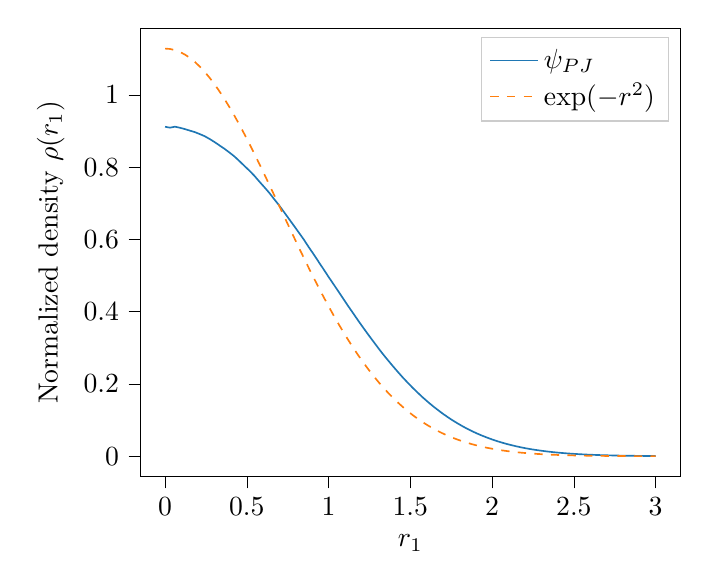
\begin{tikzpicture}

\definecolor{color0}{rgb}{0.12156862745098,0.466666666666667,0.705882352941177}
\definecolor{color1}{rgb}{1,0.498039215686275,0.0549019607843137}

\begin{axis}[
legend cell align={left},
legend style={draw=white!80.0!black},
tick align=outside,
tick pos=left,
x grid style={white!69.01960784313725!black},
xlabel={\(\displaystyle r_1\)},
xmin=-0.15, xmax=3.15,
xtick style={color=black},
y grid style={white!69.01960784313725!black},
ylabel={Normalized density \(\displaystyle \rho(r_1)\)},
ymin=-0.0562739893669188, ymax=1.18481741172113,
ytick style={color=black}
]
\addplot [semithick, color0]
table {%
0 0.911998840596385
0.0303030303030303 0.909511412757098
0.0606060606060606 0.912217763880528
0.0909090909090909 0.909272221738406
0.121212121212121 0.905621295404069
0.151515151515152 0.901364846646744
0.181818181818182 0.897263192130732
0.212121212121212 0.891848637741026
0.242424242424242 0.88585028792694
0.272727272727273 0.878201132944254
0.303030303030303 0.869590855084471
0.333333333333333 0.860255445439856
0.363636363636364 0.850937024891839
0.393939393939394 0.840672819679805
0.424242424242424 0.829851451580141
0.454545454545455 0.817066900655701
0.484848484848485 0.80383538228189
0.515151515151515 0.790811070507106
0.545454545454545 0.776781650543831
0.575757575757576 0.760781065528004
0.606060606060606 0.745399359753934
0.636363636363636 0.729706893034477
0.666666666666667 0.712077554221927
0.696969696969697 0.694767902718012
0.727272727272727 0.676074019112048
0.757575757575758 0.657101821795823
0.787878787878788 0.638249437426633
0.818181818181818 0.619094438257341
0.848484848484849 0.59982552573195
0.878787878787879 0.578782458508848
0.909090909090909 0.558777680825071
0.939393939393939 0.53797879045803
0.96969696969697 0.51740872649475
1 0.496379230413457
1.03030303030303 0.476258561363949
1.06060606060606 0.455701173127295
1.09090909090909 0.435271810642676
1.12121212121212 0.414791760936844
1.15151515151515 0.394953321348637
1.18181818181818 0.375002306575804
1.21212121212121 0.355684345568535
1.24242424242424 0.336717761498648
1.27272727272727 0.318327006135166
1.3030303030303 0.299926176615558
1.33333333333333 0.282166678552412
1.36363636363636 0.265385895284971
1.39393939393939 0.248995930032944
1.42424242424242 0.233027839304733
1.45454545454545 0.217667989556838
1.48484848484848 0.203091784494556
1.51515151515152 0.189035970255517
1.54545454545455 0.175738236082489
1.57575757575758 0.162851723361638
1.60606060606061 0.15078853996568
1.63636363636364 0.139267548148415
1.66666666666667 0.12856659562153
1.6969696969697 0.118203477653413
1.72727272727273 0.108733170132539
1.75757575757576 0.0995928551092824
1.78787878787879 0.0911912645915139
1.81818181818182 0.0832636325959449
1.84848484848485 0.0758510769293965
1.87878787878788 0.0689708360763449
1.90909090909091 0.0626954581945065
1.93939393939394 0.0568664709539298
1.96969696969697 0.0514380645217181
2 0.0464468127600457
2.03030303030303 0.0418060743665757
2.06060606060606 0.0376495485722901
2.09090909090909 0.0337459893158336
2.12121212121212 0.030314415998204
2.15151515151515 0.0270453913193502
2.18181818181818 0.0241565922009845
2.21212121212121 0.0214775996125944
2.24242424242424 0.0190996823509147
2.27272727272727 0.0170009418221463
2.3030303030303 0.0150868655919841
2.33333333333333 0.0132989711349527
2.36363636363636 0.0117689049337192
2.39393939393939 0.0103416317721274
2.42424242424242 0.00908355272982795
2.45454545454545 0.00798438326871658
2.48484848484848 0.00697442909279362
2.51515151515152 0.00609859621370828
2.54545454545455 0.00533098219757448
2.57575757575758 0.00463597852561942
2.60606060606061 0.0040343204128247
2.63636363636364 0.00350169301159901
2.66666666666667 0.00303123581359237
2.6969696969697 0.00261462555984316
2.72727272727273 0.00224160448272549
2.75757575757576 0.00193281732804632
2.78787878787879 0.00166005060198349
2.81818181818182 0.00143599506990612
2.84848484848485 0.00121976835859124
2.87878787878788 0.00104132125280946
2.90909090909091 0.000883644875226274
2.93939393939394 0.00075581675281638
2.96969696969697 0.000644771351426846
3 0.000544027404565806
};
\addlegendentry{$\psi_{PJ}$}
\addplot [semithick, color1, dashed]
table {%
0 1.12840416621713
0.0303030303030303 1.12736845801432
0.0606060606060606 1.12426703367862
0.0909090909090909 1.11911694177215
0.121212121212121 1.11194642304838
0.151515151515152 1.10279465251189
0.181818181818182 1.09171138293223
0.212121212121212 1.07875649435048
0.242424242424242 1.06399945528544
0.272727272727273 1.04751870242167
0.303030303030303 1.0294009465269
0.333333333333333 1.00974041318822
0.363636363636364 0.988638027660529
0.393939393939394 0.966200553680114
0.424242424242424 0.942539696501851
0.454545454545455 0.917771180667901
0.484848484848485 0.892013813107634
0.515151515151515 0.865388542104536
0.545454545454545 0.838017522451078
0.575757575757576 0.810023196754071
0.606060606060606 0.781527402360712
0.636363636363636 0.752650512761195
0.666666666666667 0.723510621601078
0.696969696969697 0.694222776620897
0.727272727272727 0.664898269948099
0.757575757575758 0.635643990214489
0.787878787878788 0.60656184097868
0.818181818181818 0.577748228915208
0.848484848484849 0.549293624207384
0.878787878787879 0.521282194566561
0.909090909090909 0.493791513311993
0.939393939393939 0.466892340997727
0.96969696969697 0.440648479179127
1 0.415116694083485
1.03030303030303 0.390346707196457
1.06060606060606 0.366381249106972
1.09090909090909 0.343256172373726
1.12121212121212 0.321000618690749
1.15151515151515 0.299637235239872
1.18181818181818 0.279182434824829
1.21212121212121 0.259646694183763
1.24242424242424 0.241034884771167
1.27272727272727 0.223346630282488
1.3030303030303 0.206576685258979
1.33333333333333 0.190715329250375
1.36363636363636 0.175748771220837
1.39393939393939 0.161659559151329
1.42424242424242 0.148426990110284
1.45454545454545 0.136027516425357
1.48484848484848 0.124435143983081
1.51515151515152 0.113621819101638
1.54545454545455 0.10355780085604
1.57575757575758 0.0942120161766865
1.60606060606061 0.0855523954838998
1.63636363636364 0.0775461870556947
1.66666666666667 0.0701602487474554
1.6969696969697 0.0633613160849509
1.72727272727273 0.0571162461315624
1.75757575757576 0.0513922368829435
1.78787878787879 0.0461570222645915
1.81818181818182 0.0413790430978325
1.84848484848485 0.0370275946560968
1.87878787878788 0.0330729516554313
1.90909090909091 0.0294864717109373
1.93939393939394 0.0262406784448319
1.96969696969697 0.0233093255532188
2 0.0206674432289761
2.03030303030303 0.0182913683993607
2.06060606060606 0.0161587602712191
2.09090909090909 0.0142486026865192
2.12121212121212 0.0125411947788877
2.15151515151515 0.0110181313906192
2.18181818181818 0.00966227466192603
2.21212121212121 0.00845771814269003
2.24242424242424 0.00738974470425698
2.27272727272727 0.0064447794473481
2.3030303030303 0.00561033871429013
2.33333333333333 0.00487497622162344
2.36363636363636 0.00422822723470033
2.39393939393939 0.00366055161087778
2.42424242424242 0.00316327644387662
2.45454545454545 0.00272853895014144
2.48484848484848 0.00234923014970086
2.51515151515152 0.00201893980999876
2.54545454545455 0.00173190304215185
2.57575757575758 0.00148294886561541
2.60606060606061 0.00126745098966631
2.63636363636364 0.00108128099865161
2.66666666666667 0.000920764072677906
2.6969696969697 0.000782637326292508
2.72727272727273 0.000664010804594139
2.75757575757576 0.000562331138888813
2.78787878787879 0.000475347832189927
2.81818181818182 0.000401082118214352
2.84848484848485 0.000337798315675075
2.87878787878788 0.000283977582217796
2.90909090909091 0.000238293958882928
2.93939393939394 0.000199592586080646
2.96969696969697 0.000166869965334866
3 0.000139256137083449
};
\addlegendentry{$\exp(-r^2)$}
\end{axis}

\end{tikzpicture}
    }
    \caption[One-body density using Pade-Jastrow wave function]{\label{fig:QD-benchmark-pade-jastrow-onebody}One-body density
      described by $\psi_{PJ}$ with optimized parameters. For reference, the
      exact OBD for the non-interacting system is indicated by the dotted line.\citesource{writing/scripts/QD-benchmark-onebody.py}}
\end{figure}

\begin{figure}[h]
   \centering
    \resizebox{0.7\linewidth}{!}{%
        % This file was created by matplotlib2tikz v0.7.4.
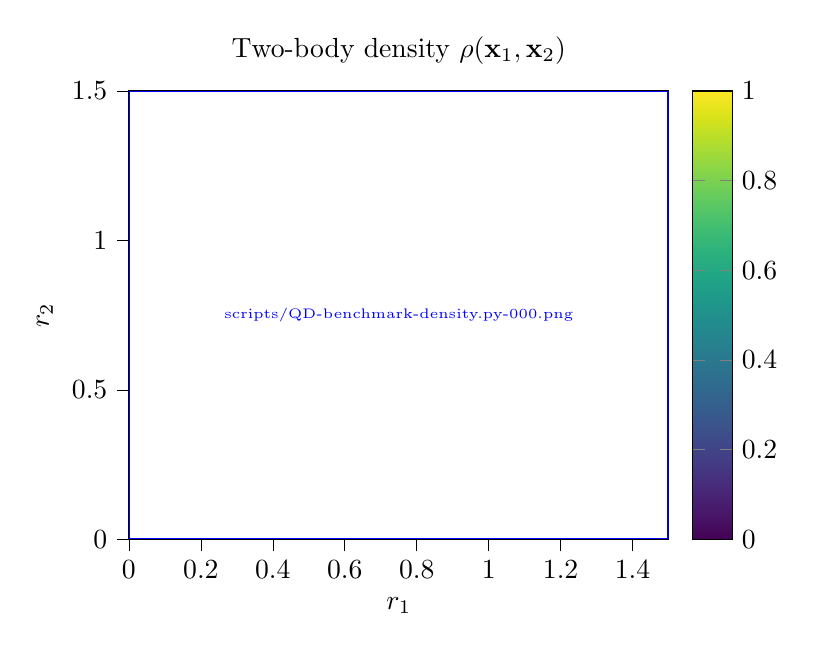
\begin{tikzpicture}

\begin{axis}[
colorbar,
colorbar style={ylabel={}},
colormap/viridis,
point meta max=1,
point meta min=0,
tick align=outside,
tick pos=left,
title={Two-body density $\rho(\mathbf{x}_1, \mathbf{x}_2)$},
x grid style={white!69.01960784313725!black},
xlabel={\(\displaystyle r_1\)},
xmin=0, xmax=1.5,
xtick style={color=black},
y grid style={white!69.01960784313725!black},
ylabel={\(\displaystyle r_2\)},
ymin=0, ymax=1.5,
ytick style={color=black}
]
\addplot graphics [includegraphics cmd=\pgfimage,xmin=0, xmax=1.5, ymin=0, ymax=1.5] {scripts/QD-benchmark-density.py-000.png};
\end{axis}

\end{tikzpicture}
    }
    \resizebox{0.7\linewidth}{!}{%
        % This file was created by matplotlib2tikz v0.7.4.
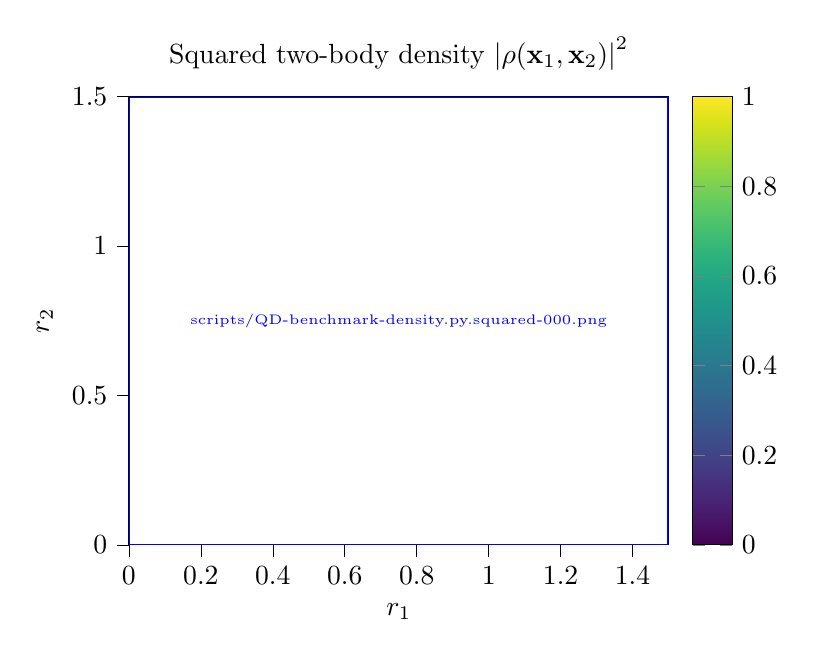
\begin{tikzpicture}

\begin{axis}[
colorbar,
colorbar style={ylabel={}},
colormap/viridis,
point meta max=1,
point meta min=0,
tick align=outside,
tick pos=left,
title={Squared two-body density $\left|\rho(\mathbf{x}_1, \mathbf{x}_2)\right|^2$},
x grid style={white!69.01960784313725!black},
xlabel={\(\displaystyle r_1\)},
xmin=0, xmax=1.5,
xtick style={color=black},
y grid style={white!69.01960784313725!black},
ylabel={\(\displaystyle r_2\)},
ymin=0, ymax=1.5,
ytick style={color=black}
]
\addplot graphics [includegraphics cmd=\pgfimage,xmin=0, xmax=1.5, ymin=0, ymax=1.5] {scripts/QD-benchmark-density.py.squared-000.png};
\end{axis}

\end{tikzpicture}
    }
    \caption[Two-body density using Pade-Jastrow wave function]{\label{fig:QD-benchmark-pade-jastrow-density}Top: Two-body density
      described by $\psi_{PJ}$ with optimized parameters. Bottom: The squared
      equivalent of the top figure, included to emphasize the small decrease in
      density along the diagonal $r_1=r_2$.\citesource{writing/scripts/QD-benchmark-density.py}}
\end{figure}

\clearpage


\section{Restricted Boltzmann Machine}

\begin{figure}[h]
  \centering
  \tikzstyle{neuron}=[draw,circle,minimum size=20pt,inner sep=0pt, fill=white]
\tikzstyle{stateTransition}=[thick]
\tikzstyle{learned}=[text=red]
\begin{tikzpicture}[scale=2]
  % \draw ;
  \draw[fill=black!30, rounded corners] (-0.2, -0.2) rectangle (3.2, 0.2) {};
  \draw[fill=black!30, rounded corners] (0.3, 0.8) rectangle (2.7, 1.2) {};

  \node (v1)[neuron] at (0, 0) {$x_1$};
  \node (v2)[neuron] at (1, 0) {$x_2$};
  \node (v3)[neuron] at (2, 0) {$x_3$};
  \node (v4)[neuron] at (3, 0) {$x_4$};
  \node[right=0.1cm of v4] (v) {$\vx \in \mathbb{R}^{P\cdot D}$};
  \node[learned,below=0.1cm of v1] (bv1) {$a_{1}$};
  \node[learned,below=0.1cm of v2] (bv2) {$a_{2}$};
  \node[learned,below=0.1cm of v3] (bv3) {$a_{3}$};
  \node[learned,below=0.1cm of v4] (bv4) {$a_{4}$};

  \node (h1)[neuron] at (0.5, 1) {$h_1$};
  \node (h2)[neuron] at (1.5, 1) {$h_2$};
  \node (h3)[neuron] at (2.5, 1) {$h_3$};
  \node[right=0.1cm of h3] (h) {$\vb{h} \in \{0, 1\}^3$};
  \node[learned,above=0.1cm of h1] (bh1) {$b_{1}$};
  \node[learned,above=0.1cm of h2] (bh2) {$b_{2}$};
  \node[learned,above=0.1cm of h3] (bh3) {$b_{3}$};

  \draw[learned,stateTransition] (v1) -- (h1) node [midway,above=-0.06cm,sloped] {$W_{1,1}$};
  \draw[stateTransition] (v1) -- (h2) node [midway,above=-0.06cm,sloped] {};
  \draw[stateTransition] (v1) -- (h3) node [midway,above=-0.06cm,sloped] {};

  \draw[stateTransition] (v2) -- (h1) node [midway,above=-0.06cm,sloped] {};
  \draw[stateTransition] (v2) -- (h2) node [midway,above=-0.06cm,sloped] {};
  \draw[stateTransition] (v2) -- (h3) node [midway,above=-0.06cm,sloped] {};

  \draw[stateTransition] (v3) -- (h1) node [midway,above=-0.06cm,sloped] {};
  \draw[stateTransition] (v3) -- (h2) node [midway,above=-0.06cm,sloped] {};
  \draw[stateTransition] (v3) -- (h3) node [midway,above=-0.06cm,sloped] {};

  \draw[stateTransition] (v4) -- (h1) node [midway,above=-0.06cm,sloped] {};
  \draw[stateTransition] (v4) -- (h2) node [midway,above=-0.06cm,sloped] {};
  \draw[learned,stateTransition] (v4) -- (h3) node [midway,above=-0.06cm,sloped] {$W_{4,3}$};
\end{tikzpicture}
  \caption[Illustration of a Restricted Boltzmann Machine (RBM)]{Example diagram of a Guassian-Binary Restricted Boltzmann Machine, showed with four visible nodes
    and three hidden nodes. The red values are the parameters, and consist of
    visible layer bias, $\vb a$, hidden layer bias, $\vb b$ and connection
    weights $\mat W$.\citesource{writing/illustrations/rbm-diagram.tex}}
  \label{fig:rbm-diagram-example}
\end{figure}


The first ML-inspired model we have applied is a Restricted Boltzmann Machine (RBM).
This type of model has seen a significant rise in usage
since~\textcite{Carleo602} demonstrated the RBMs capability to
represent the wave function for some selected Hamiltonians. All the
Hamiltonians for which they showed successful results, however, had discrete
configuration spaces. The current system is continuous as the particles can have
any real valued coordinates, and so the type of RBM must change as well.

While more than one choice exist, we have used a Gaussian-Binary RBM\@.
\cref{fig:rbm-diagram-example} shows and example diagram of the network
structure. \textcite{Flugsrud-2018} has a full introduction to RBMs, including
all details needed for \gls{vmc}\@. For our purposes it suffices to say that the
resulting wave function looks as follows:

\begin{align}
  \label{eq:rbm-def}
  \psi_{RBM}(\vX) &=
        e^{-\sum_i^{M} \frac{\qty(X_i-a_i)^2}{2\sigma^2}}
        \prod_j^N \qty(1 + e^{b_j+\sum_i^M \frac{X_iW_{ij}}{\sigma^2}}),
\end{align}
where $M = P\cdot D$ is the number of degrees of freedom and $N$ is the number
of hidden nodes. Note also that $X_i$ in the above refers to the $i$'th degree
of freedom, counting through $\mat X$ in row major order. The parameters are
$\vb a, \vb b$ and $\mat W$, and we hold $\sigma^2=1$ constant in this case.

If we set $\vb a = \vb 0$ we can recognize the first factor of~\cref{eq:rbm-def}
as the non-interacting ground state. That way we can consider the second factor
the Jastrow factor introduced by the RBM structure. It has an unconventional
form, as it is not a pure exponential.


\subsection{Optimizing}

We produced the following with normally distributed random
initial values for the parameters, running $\num{60000}$ optimization steps with
$\num{2000}$ \gls{mc} cycles each. We have also once again used \acrlong{is}
and ADAM\@. A new addition (not strictly necessary for similar results) is the use
of mild $L2$ regularization, which serves to drive parameters that do not
contribute towards zero. The results are similar for different hyper-parameter
choices, and the above is simply one such example.

\cref{fig:QD-rbm-training} shows the ground state energy as a function of
training steps, along with the progression of the variational
parameters. While we see a clear improvement in the initial stages, the RBM
fails to converge as accurately as the benchmark. \cref{tab:rbm-energy-results}
shows the precise results of the final model. While slightly different results
are possible with different training settings, we have never observed the RBM
achieve energies below $\SI{3.07}{\au}$, which is an error of about two orders
of magnitude larger than the benchmark.



\begin{figure}[h]
   \centering
    \resizebox{\linewidth}{!}{%
        % This file was created by matplotlib2tikz v0.7.4.
\begin{tikzpicture}

\definecolor{color0}{rgb}{0.12156862745098,0.466666666666667,0.705882352941177}
\definecolor{color1}{rgb}{1,0.498039215686275,0.0549019607843137}
\definecolor{color2}{rgb}{0.172549019607843,0.627450980392157,0.172549019607843}
\definecolor{color3}{rgb}{0.83921568627451,0.152941176470588,0.156862745098039}
\definecolor{color4}{rgb}{0.580392156862745,0.403921568627451,0.741176470588235}
\definecolor{color5}{rgb}{0.549019607843137,0.337254901960784,0.294117647058824}
\definecolor{color6}{rgb}{0.890196078431372,0.466666666666667,0.76078431372549}
\definecolor{color7}{rgb}{0.737254901960784,0.741176470588235,0.133333333333333}
\definecolor{color8}{rgb}{0.0901960784313725,0.745098039215686,0.811764705882353}

\begin{groupplot}[group style={group size=2 by 1}]
\nextgroupplot[
legend cell align={left},
legend style={draw=white!80.0!black},
tick align=outside,
tick pos=left,
x grid style={white!69.01960784313725!black},
xlabel={\% of training},
ylabel={Ground state energy $[\si{\au}]$},
xmin=-5, xmax=105,
xtick style={color=black},
y grid style={white!69.01960784313725!black},
ylabel={Ground state energy (a.u.)},
ymin=2.98661068407909, ymax=3.28117563433902,
ytick style={color=black},
ylabel near ticks,
]
\addplot [semithick, color0]
table {%
0 3.26778631841812
1 3.14947938985174
2 3.08688912225823
3 3.08885451515261
4 3.09177410749784
5 3.09004525149916
6 3.0825541152983
7 3.08659830244641
8 3.08807346743545
9 3.08737072593149
10 3.08486888597368
11 3.08340761872365
12 3.08002103093302
13 3.08066509425232
14 3.08064724852931
15 3.0811325959243
16 3.08266140122991
17 3.07803865434052
18 3.07917375658203
19 3.07963901513708
20 3.07648725941841
21 3.08228553442701
22 3.07539106757631
23 3.07763127655871
24 3.07655428552753
25 3.07897182953364
26 3.08394594524133
27 3.08645322727406
28 3.082840787604
29 3.08068617245471
30 3.07836864155134
31 3.07921967769809
32 3.0790717484034
33 3.08201042139664
34 3.08488869616681
35 3.08604729702945
36 3.08348269965668
37 3.08521472731162
38 3.07849701860954
39 3.08451618888308
40 3.07831379169806
41 3.0817796559986
42 3.08292317194317
43 3.07993230566767
44 3.07640939000394
45 3.08087346092422
46 3.08058861137909
47 3.08001983078223
48 3.07761412644538
49 3.08610665192563
50 3.0813639637218
51 3.085521487051
52 3.0755401337017
53 3.08078022649304
54 3.07671814464576
55 3.08964303049499
56 3.0833480006293
57 3.07927864274738
58 3.07930757914846
59 3.07644874796548
60 3.07849958420558
61 3.08074328833594
62 3.07716301482793
63 3.08019863403575
64 3.08076955667335
65 3.08349780114468
66 3.0974741178163
67 3.07468187863078
68 3.07764140737187
69 3.0852065893175
70 3.08154362931524
71 3.0859197476721
72 3.08036312538626
73 3.08003121148469
74 3.07807609707624
75 3.08051735873207
76 3.07676654485076
77 3.077092807589
78 3.07723286080184
79 3.0774235331529
80 3.07924843845931
81 3.07832455119813
82 3.07745195139007
83 3.07494597671178
84 3.08148728802571
85 3.07865090379405
86 3.07976191585688
87 3.08699874854927
88 3.08083335491312
89 3.07882722252863
90 3.07886516337923
91 3.07881701675731
92 3.07454498423968
93 3.07734877499453
94 3.08619177869686
95 3.07443726356216
96 3.07844469746873
97 3.08239296752874
98 3.07912115499406
99 3.07938525071009
100 3.0787187826413
};
\addlegendentry{$\langle E_L\rangle$}
\addplot [semithick, black, opacity=0.5, dashed]
table {%
-5 3
105 3
};
\addlegendentry{Exact}

\nextgroupplot[
tick align=outside,
tick pos=left,
x grid style={white!69.01960784313725!black},
xlabel={\% of training},
ylabel={Parameters},
xmin=-5, xmax=105,
xtick style={color=black},
y grid style={white!69.01960784313725!black},
ymin=-1.03556808440274, ymax=1.05857039605435,
ytick style={color=black},
ylabel near ticks,
ytick pos=right,
yticklabel pos=right,
ylabel style={rotate=-180},
]
\addplot [semithick, color0]
table {%
0 -0.117841969177496
1 -0.118284580859272
2 -0.147608196627473
3 -0.151476232340979
4 -0.161526852251141
5 -0.178177036893419
6 -0.184745040018205
7 -0.205690835570629
8 -0.231359339255245
9 -0.261957638762584
10 -0.291210806627067
11 -0.301131326969523
12 -0.345276125459561
13 -0.384083771771859
14 -0.426541570963376
15 -0.460732756268614
16 -0.521931907667269
17 -0.559987111617287
18 -0.588345868758849
19 -0.61298066432494
20 -0.654170151960175
21 -0.690641640079611
22 -0.686238687831283
23 -0.683465897548257
24 -0.695031030597753
25 -0.692580372744827
26 -0.706077028354332
27 -0.695129476076795
28 -0.700824232546135
29 -0.702201551573074
30 -0.701060363260462
31 -0.695954452438
32 -0.687008552536897
33 -0.703708909757854
34 -0.675566499950374
35 -0.690815051377925
36 -0.679702143904449
37 -0.694707347240377
38 -0.698010592748375
39 -0.698369986923307
40 -0.696915581834592
41 -0.674469260817328
42 -0.714023859148464
43 -0.708975374785558
44 -0.729003559361711
45 -0.691231814282918
46 -0.693192555380428
47 -0.704205376167331
48 -0.689699119861733
49 -0.714972001021041
50 -0.704259416870179
51 -0.694003624283448
52 -0.707638328510849
53 -0.698142704730003
54 -0.684634110943013
55 -0.705673541387552
56 -0.70165459652634
57 -0.712141716860302
58 -0.703220675026353
59 -0.696443139244194
60 -0.689258032975759
61 -0.706475314606333
62 -0.699144265460016
63 -0.689358733191036
64 -0.689816011697235
65 -0.700501424208051
66 -0.708612101944233
67 -0.694924513112424
68 -0.695563465278716
69 -0.686080509555422
70 -0.70408429278159
71 -0.709716623804077
72 -0.712428257596636
73 -0.703787042982799
74 -0.689308950583273
75 -0.691330331833291
76 -0.682303634294363
77 -0.697967874522511
78 -0.696416661192705
79 -0.696313872921052
80 -0.714946220503201
81 -0.705090159110704
82 -0.689035996798875
83 -0.699470311461095
84 -0.696675213706153
85 -0.686927489256884
86 -0.70551423437382
87 -0.700283695676133
88 -0.704363545298113
89 -0.67420772658133
90 -0.701153425631444
91 -0.702688101948318
92 -0.707625879200657
93 -0.701169936874863
94 -0.687166519895171
95 -0.705539786016749
96 -0.682868835354953
97 -0.703729777662518
98 -0.697633195405716
99 -0.705297109742872
100 -0.700929372490184
};
\addplot [semithick, color1]
table {%
0 -0.168517826694971
1 -0.116174681839336
2 -0.0237820443114784
3 -0.045509537555996
4 -0.0412411960005719
5 -0.0872885903411773
6 -0.106709285448678
7 -0.126759758439932
8 -0.148928359317894
9 -0.166584134981256
10 -0.168512585700758
11 -0.185253863692317
12 -0.179619950987432
13 -0.161906247273137
14 -0.164391107447321
15 -0.15570851047042
16 -0.141998136122209
17 -0.171690505265161
18 -0.177118655545456
19 -0.148698717936924
20 -0.170693321569304
21 -0.180295202934484
22 -0.175645852783201
23 -0.164622856533075
24 -0.182515761753992
25 -0.182042895013969
26 -0.178474934469043
27 -0.170422760971178
28 -0.168365442323457
29 -0.20541425216402
30 -0.176092545377143
31 -0.189588277974403
32 -0.186556648364522
33 -0.184450310761327
34 -0.193448632162503
35 -0.185826460518535
36 -0.180433077137332
37 -0.194779879746444
38 -0.176940685377482
39 -0.200109160438354
40 -0.185904039243833
41 -0.18609159048158
42 -0.1952880288162
43 -0.187120030418775
44 -0.184428202353413
45 -0.189501752870751
46 -0.175358827313395
47 -0.197793636458806
48 -0.196740663178943
49 -0.169963068431848
50 -0.193267988366865
51 -0.195139646173826
52 -0.184683854810395
53 -0.177255285552054
54 -0.199307678800736
55 -0.204875800953848
56 -0.19169146002929
57 -0.183554537215395
58 -0.204478776760284
59 -0.180106825643502
60 -0.180900075169887
61 -0.189459117613751
62 -0.205594335745631
63 -0.188013559718387
64 -0.199141270108549
65 -0.17994790736683
66 -0.203811415796159
67 -0.197864013888265
68 -0.197616899935467
69 -0.186473594374254
70 -0.200809573081615
71 -0.206724654667035
72 -0.209341474626318
73 -0.19975778493527
74 -0.192287680219868
75 -0.201015577272785
76 -0.194996816538647
77 -0.190931967861276
78 -0.181041097661161
79 -0.174470529288789
80 -0.200534364087405
81 -0.180116971053231
82 -0.174517753623464
83 -0.179247367938286
84 -0.197195547587956
85 -0.175300162764342
86 -0.201034810418223
87 -0.179814669328689
88 -0.184230338588902
89 -0.193777797324401
90 -0.175785531428736
91 -0.183712053164084
92 -0.168336728169393
93 -0.183289651000195
94 -0.180835853499765
95 -0.187224466381638
96 -0.185698440902889
97 -0.202071550282589
98 -0.19984109267011
99 -0.172071137777818
100 -0.186967150573917
};
\addplot [semithick, color2]
table {%
0 0.0578126847448953
1 0.0239691020502556
2 0.0622739143668992
3 0.0570222698023475
4 0.0766115907542125
5 0.0855841689657839
6 0.098824941580093
7 0.12404260098867
8 0.157952210276348
9 0.169676773156474
10 0.207968861719094
11 0.230189840426506
12 0.272328014975971
13 0.315552074549481
14 0.367348735513422
15 0.411174026554853
16 0.466970288079056
17 0.517286993678151
18 0.544717738654154
19 0.594325817092425
20 0.619897190632202
21 0.615301665469338
22 0.642263479369982
23 0.64685816029142
24 0.668979666327317
25 0.665464707695501
26 0.677092989994602
27 0.669739111359179
28 0.665372665595139
29 0.686206562071545
30 0.680784138975695
31 0.663049425837883
32 0.685685730521279
33 0.682999012945518
34 0.697306577707432
35 0.676219851886695
36 0.6940694604607
37 0.693411176357958
38 0.684868913939419
39 0.693262204414279
40 0.674702975246693
41 0.699503344408849
42 0.698529456918059
43 0.699509929604414
44 0.701204742477404
45 0.68749293877115
46 0.681013485011589
47 0.704964315856105
48 0.696725500881738
49 0.689733222743377
50 0.690633829368131
51 0.688879659097443
52 0.694521777154383
53 0.680883699072709
54 0.697819458740834
55 0.699421293105179
56 0.70012827394827
57 0.686586721374614
58 0.714291500144085
59 0.690147638269807
60 0.710268509671175
61 0.69364943022072
62 0.689880152479791
63 0.69427653051402
64 0.69171179927545
65 0.696162353132352
66 0.704802270963466
67 0.692995323445902
68 0.713897163949585
69 0.708002983068241
70 0.679513259300539
71 0.692966709888001
72 0.696895322421662
73 0.700481953698286
74 0.690581431273791
75 0.68536139221896
76 0.67802575188554
77 0.683093828649745
78 0.68758862651364
79 0.698301793251585
80 0.703021850798983
81 0.696429331260115
82 0.697988025385607
83 0.681965294949251
84 0.695703860951957
85 0.694252751572036
86 0.697020417853841
87 0.695613180216285
88 0.693806967167993
89 0.686742976325609
90 0.711861546827682
91 0.692136812380934
92 0.691350066816511
93 0.711624053866064
94 0.697124522625767
95 0.692834927783465
96 0.682736923440414
97 0.693754055894466
98 0.696698426316794
99 0.684833227965497
100 0.685116360081513
};
\addplot [semithick, color3]
table {%
0 0.183287074758229
1 0.132429481752042
2 0.0389640782807688
3 0.0657472578380956
4 0.0775976895420614
5 0.0862421974007416
6 0.142899213546159
7 0.161880437934315
8 0.173630092674005
9 0.201748690484137
10 0.195711198526497
11 0.192918318655036
12 0.180658409582405
13 0.175923834282281
14 0.19371460907686
15 0.183537293971219
16 0.177749852818179
17 0.180061551614179
18 0.177078272065152
19 0.181745805912424
20 0.164952620328332
21 0.175816500797101
22 0.171481607143277
23 0.174032037976757
24 0.186969669252365
25 0.182959411901719
26 0.187899813971458
27 0.191223494569405
28 0.185530437785418
29 0.19992167157473
30 0.188753704326813
31 0.188883420586678
32 0.205062510580702
33 0.17556783485388
34 0.218452013027873
35 0.198405965221406
36 0.194757077875679
37 0.208645904197481
38 0.187850879152027
39 0.194536709255283
40 0.19206095254628
41 0.170493529680027
42 0.204285057087975
43 0.196649398826768
44 0.195483748470771
45 0.195966988315664
46 0.16326969240153
47 0.194943976245223
48 0.189282911178688
49 0.223920866951644
50 0.185675556285813
51 0.206525635999128
52 0.192480185170143
53 0.176928706827285
54 0.195887311098028
55 0.187030604007873
56 0.184334721254913
57 0.20143965384844
58 0.194831948028397
59 0.220213152691589
60 0.192085332965006
61 0.187219815856679
62 0.192696270339148
63 0.183372063265722
64 0.195086686706335
65 0.187439941508585
66 0.200291479138498
67 0.192129476874698
68 0.195891251373809
69 0.186357463905647
70 0.191333810810809
71 0.195207560461176
72 0.208428608590187
73 0.198762035814046
74 0.178424729287923
75 0.171486782975363
76 0.192088065952442
77 0.184852921088306
78 0.196045956179313
79 0.181855183214294
80 0.18586940988296
81 0.185040377825289
82 0.187500043649283
83 0.193373988336058
84 0.168744836639204
85 0.199614890095825
86 0.172481725649594
87 0.166273150543282
88 0.179830347437683
89 0.198731472953572
90 0.195616771862649
91 0.188804362480916
92 0.190846083876476
93 0.183124611766118
94 0.194625111549432
95 0.168130154502491
96 0.183853267131626
97 0.183502983448932
98 0.179683757825927
99 0.185130876358602
100 0.180034979038336
};
\addplot [semithick, color4]
table {%
0 -0.137779610369542
1 -0.136937979892395
2 -0.0883592401185548
3 -0.0759296966030259
4 -0.0520952958777989
5 -0.0307572076762653
6 -0.0759098785997443
7 -0.0824171842469352
8 -0.0155793500732775
9 -0.0444361235560702
10 -0.0415661812123278
11 -0.0539319774248856
12 -0.0443577980583036
13 -0.0408636053242552
14 -0.0363023492039638
15 -0.0283237187440424
16 -0.0551033435805871
17 -0.0580216911782531
18 -0.0662746524076453
19 -0.0358261670773747
20 -0.056466627836234
21 -0.027626949040093
22 -0.0340606595746497
23 -0.00470877211849913
24 -0.0522075868117601
25 -0.00969091780504367
26 -0.0179670349525436
27 0.0178047762034177
28 0.00221114492838966
29 -0.00182677270046398
30 -0.00258202818677059
31 -0.00698757875348517
32 -0.0470266457302778
33 -0.0154395827988023
34 -0.0649750606099243
35 -0.0433032734994719
36 -0.0355542832793026
37 -0.0290234386901202
38 -0.0339227902530721
39 -0.0246360090291442
40 -0.00237390721626307
41 -0.00208697112403829
42 -0.0368384156375818
43 -0.0094282254607214
44 -0.0478995651191059
45 -0.0114003769919481
46 0.0256708807928039
47 -0.0303861655852825
48 0.0100238448867629
49 -0.0291563639278864
50 -0.0389513202755132
51 -0.0318823925294402
52 -0.0280949188427158
53 -0.00629452836389987
54 -0.00688472858890938
55 0.00988212723348274
56 0.00530323375829856
57 -0.0133038248122804
58 -0.0213183632799106
59 -0.00116352769881812
60 -0.000142107558771265
61 0.00326342918826165
62 -0.0127645112409538
63 -0.00263068989998797
64 -0.0260467020749329
65 -0.0122859943274085
66 -0.0232273498230273
67 -0.00398018816928315
68 -0.0235829687401191
69 0.0153238724460127
70 -0.0247437816172799
71 -0.0254275867185743
72 -0.0348281956711
73 -0.0312713204826211
74 -0.00651885620782185
75 -0.0264032175610295
76 -0.0265624955381769
77 -0.0190003766864374
78 -0.0016543028749428
79 -0.0334193254670314
80 -0.0457731292803179
81 -0.0162721930347208
82 -0.00697863918601924
83 0.0374349667463795
84 -0.00535457039306125
85 0.0115695225478509
86 -0.034423773615372
87 0.0092139748117145
88 0.00652262783093436
89 0.00844333057161675
90 -0.0528632334485723
91 -0.000694414145357467
92 0.00513653996283588
93 -0.0280267427662427
94 -0.0384508736062291
95 -0.021214529408253
96 -0.0141942491109538
97 -0.0611973591139666
98 -0.0469820600735964
99 -0.00343150076332478
100 -0.0100598469829275
};
\addplot [semithick, color5]
table {%
0 0.035092500313306
1 -0.0861822678049885
2 -0.127367559245924
3 -0.0874432623784901
4 -0.0817434508706693
5 -0.0677911905187272
6 -0.0398810650801974
7 -0.0329043021735603
8 -0.0353803327205786
9 -0.0533234745522923
10 -0.090276221510884
11 -0.102310274460065
12 -0.111574468577508
13 -0.134491025470206
14 -0.132825894110224
15 -0.131113541263183
16 -0.137361328468543
17 -0.126419595530195
18 -0.136936252486358
19 -0.13233361652405
20 -0.158313455095911
21 -0.183002693496246
22 -0.186348569980816
23 -0.182159487198703
24 -0.333772717673867
25 -0.248020487380919
26 -0.214044951930013
27 -0.240915024687131
28 -0.224510177823057
29 -0.187896083112768
30 -0.209737340484752
31 -0.239848962320034
32 -0.221481744414614
33 -0.199415044734208
34 -0.193155609107824
35 -0.241408146883695
36 -0.234367035994861
37 -0.261107638692642
38 -0.229054608895576
39 -0.256194031880803
40 -0.241640730291495
41 -0.260972439938678
42 -0.233617605175208
43 -0.280258532639826
44 -0.255621331081189
45 -0.26723505544152
46 -0.242793935706818
47 -0.257278401483627
48 -0.20321653037851
49 -0.296042381621783
50 -0.234789191028638
51 -0.26878041394595
52 -0.317425431204237
53 -0.226655613045935
54 -0.246049091123516
55 -0.167707909475823
56 -0.166000201349949
57 -0.224422461787242
58 -0.262277114338316
59 -0.275686160121517
60 -0.272437512637225
61 -0.27801710012176
62 -0.19010269660309
63 -0.25378171451453
64 -0.250490341708053
65 -0.338313182760493
66 -0.247381257872765
67 -0.225399323300402
68 -0.228418423373035
69 -0.278898001989736
70 -0.297403857659968
71 -0.217442623976893
72 -0.186559627010419
73 -0.381647814133918
74 -0.218130555788455
75 -0.27657113953966
76 -0.175979632708966
77 -0.20595318553399
78 -0.244679050154886
79 -0.199933883338751
80 -0.193636105616554
81 -0.253127018589654
82 -0.189180117914464
83 -0.284267265009544
84 -0.240835642469927
85 -0.231376727625655
86 -0.265365733051995
87 -0.232930566479254
88 -0.209480340257955
89 -0.183801115357132
90 -0.197981746911258
91 -0.210579277760183
92 -0.266103009393965
93 -0.299393719404831
94 -0.270869937841552
95 -0.245823284080621
96 -0.241555787415371
97 -0.288541603303101
98 -0.20221207262901
99 -0.263991224438291
100 -0.269974079519619
};
\addplot [semithick, color6]
table {%
0 -0.144743482433268
1 -0.134061025577377
2 -0.0624524383444256
3 -0.0681789751772014
4 -0.0532538392091842
5 -0.0548186511245464
6 -0.083748389257064
7 -0.0330254199856477
8 -0.0192767990627175
9 -0.0334528557389933
10 0.0115983678495587
11 0.0316925782446146
12 0.0447459203568569
13 0.0756848178763574
14 0.098959916117016
15 0.10497911731242
16 0.127978706161942
17 0.127772245430811
18 0.103781647685905
19 0.0841660213868786
20 0.0363624565440729
21 -0.0183061294592857
22 -0.0593735030054122
23 -0.0910754542021116
24 -0.238182000376647
25 -0.208877785515179
26 -0.194263930373288
27 -0.21649839295981
28 -0.210430664533909
29 -0.188652298204955
30 -0.20126210368189
31 -0.234419049721137
32 -0.215163998009109
33 -0.204539616651082
34 -0.182026908678248
35 -0.236154399002207
36 -0.224507125359404
37 -0.25471894988242
38 -0.229568378223817
39 -0.25637613822981
40 -0.241548486750939
41 -0.259006922749968
42 -0.234332962121301
43 -0.277875054385455
44 -0.256708262715272
45 -0.26867289643004
46 -0.243454718096918
47 -0.257109138950448
48 -0.203644412066994
49 -0.293780891357521
50 -0.23508798487324
51 -0.268292758576046
52 -0.317603241865034
53 -0.226820815825593
54 -0.24595076188124
55 -0.168002936623127
56 -0.166135509324588
57 -0.2241861914102
58 -0.262196732080478
59 -0.275403733655406
60 -0.272312896564855
61 -0.27804726837267
62 -0.190158413882081
63 -0.25375477719795
64 -0.25048875168738
65 -0.338289084309062
66 -0.247381714603421
67 -0.225396895294042
68 -0.228401027980755
69 -0.278860079019857
70 -0.297423521240624
71 -0.21745501861486
72 -0.186560279147583
73 -0.381634564352989
74 -0.218154132414842
75 -0.27658582498708
76 -0.175984654043789
77 -0.205965263099859
78 -0.244676445215255
79 -0.199929117162813
80 -0.193647960884266
81 -0.253127402765016
82 -0.189178016783298
83 -0.284257554628864
84 -0.240842399558694
85 -0.231370080538972
86 -0.26537095880168
87 -0.232933277972366
88 -0.209481569535001
89 -0.183799012285928
90 -0.197980178561512
91 -0.210578678178436
92 -0.2661008562555
93 -0.299393402294522
94 -0.270868944303222
95 -0.245824464826369
96 -0.241556030773985
97 -0.288542602787214
98 -0.20221305261247
99 -0.26399085282688
100 -0.269974472831171
};
\addplot [semithick, white!49.80392156862745!black]
table {%
0 -0.0151524271686803
1 -0.0913183015721587
2 -0.129856608124111
3 -0.094513391348125
4 -0.0814417795742177
5 -0.0798100558368352
6 -0.0207877738007846
7 -0.0614710584400028
8 -0.0494776666981612
9 -0.0405190492766855
10 -0.0640515031014897
11 -0.0418542694148258
12 -0.0324149145043087
13 -0.0608249625773501
14 -0.0563851811238518
15 -0.0421377574057834
16 -0.0748456286785623
17 -0.0761960775966097
18 -0.0825163439262087
19 -0.0825349927451225
20 -0.0708469227157535
21 -0.069209734212321
22 -0.0404906719870282
23 -0.0224742060570746
24 -0.0358067330866515
25 -0.0282608608993036
26 -0.0281801595944008
27 -0.0210811043047623
28 -0.02568620342767
29 0.00719083918959043
30 -0.0262925541095772
31 -0.0182378692159596
32 -0.0167911334550508
33 -0.0185180804419946
34 -0.0123037292229249
35 -0.0205161496917184
36 -0.00124669763006091
37 -0.0191821070880497
38 -0.0357413416294931
39 -0.0432993717364893
40 -0.0488351836555899
41 -0.00771328557611957
42 -0.00730029439162058
43 0.0143939606112296
44 -0.00349587120197966
45 0.0458464975662798
46 -0.00405767532845159
47 -0.0400172798834284
48 -0.0502253921782351
49 -0.0475557330276617
50 -0.0391037794909719
51 -0.034299568300274
52 -0.0398705577822238
53 -0.040362880001581
54 -0.0157456088107293
55 -0.0512795324207387
56 -0.0525436117977158
57 -0.0147237930536626
58 -0.033661132756271
59 -0.0174786131764528
60 -0.0301333122407204
61 -0.0223624406192437
62 -0.0234556886979485
63 -0.0276418579090159
64 -0.00334814705175983
65 -0.0391119305709429
66 -0.0186081407873672
67 -0.0392296949098633
68 -0.0472601072470643
69 -0.0505223848724599
70 -0.030787989733405
71 -0.0226784850273241
72 -0.0222959882703397
73 -0.00576706370624396
74 -0.0255646041380676
75 -0.0212629945410975
76 -0.00339079428875706
77 -0.0207011727257665
78 -0.0148346241088344
79 -0.0349322250926083
80 -0.046149790962858
81 -0.0288791024465654
82 -0.0310033589088809
83 -0.00540455207237805
84 0.00434757825070736
85 -0.0391035678548132
86 -0.0571549329226187
87 -0.030617286302665
88 -0.0370086522491138
89 0.0100021024359211
90 -0.0215556143500916
91 -0.000846118544716431
92 -0.0124659809726186
93 -0.022423652439006
94 -0.0422869068261843
95 -0.0443451795715016
96 -0.00496974330239706
97 -0.0151316062536292
98 -0.0357564793598738
99 -0.0248755861628915
100 -0.0170723701890036
};
\addplot [semithick, color7]
table {%
0 0.185740813824724
1 0.564400702060892
2 0.430310241373172
3 0.428117645181848
4 0.438587903219415
5 0.435875734664948
6 0.469018381906866
7 0.465244558600847
8 0.474669606916768
9 0.497878121318511
10 0.489189879457369
11 0.481191026407585
12 0.491685914324221
13 0.488078909144776
14 0.536714207402653
15 0.542254490394387
16 0.531540517712119
17 0.504225646427518
18 0.513711201943898
19 0.526824265206809
20 0.517419939237025
21 0.53900177820525
22 0.52268899899133
23 0.515845763196493
24 0.50464382105214
25 0.543672965887466
26 0.522965894666593
27 0.534148312353307
28 0.548355570378578
29 0.540135073123262
30 0.510093954667188
31 0.513944745940331
32 0.529567350989963
33 0.500872803286468
34 0.534315445888809
35 0.523953481500412
36 0.529418080685294
37 0.519232594444793
38 0.503867862033345
39 0.520242329939718
40 0.503152676136154
41 0.541175219672546
42 0.528651060143593
43 0.509392576261098
44 0.537660479636029
45 0.515712594445901
46 0.511512778367004
47 0.501740072620905
48 0.513867497010957
49 0.500456803897535
50 0.515300827539893
51 0.492120130819322
52 0.497955498558031
53 0.519310036084187
54 0.518943722680145
55 0.515656505687258
56 0.511396780405527
57 0.516546250967337
58 0.521396810297285
59 0.520308585548292
60 0.516098437422695
61 0.505658073275023
62 0.503866374166173
63 0.529444155652338
64 0.508675030170382
65 0.490082825430173
66 0.507607682720173
67 0.502775154645144
68 0.507398593950118
69 0.506988845612875
70 0.520679540209823
71 0.522484653824316
72 0.518673610308731
73 0.525084311009008
74 0.501635952824381
75 0.517308135666404
76 0.51788874964763
77 0.518435663898113
78 0.534758626915488
79 0.516302772846408
80 0.53752440103309
81 0.513931210459752
82 0.524659342557633
83 0.51108529273048
84 0.511335054721793
85 0.54160604151172
86 0.522644085167516
87 0.547571737272739
88 0.540710202947581
89 0.535843884776325
90 0.526085596817978
91 0.517610867641372
92 0.506837434116663
93 0.523400424636136
94 0.542384889365546
95 0.529725847968781
96 0.528757290055282
97 0.509835821422129
98 0.538096588069685
99 0.528950118300225
100 0.500594568043341
};
\addplot [semithick, color8]
table {%
0 -0.127210769859985
1 -0.309143690842585
2 -0.188826680942468
3 -0.158572728032208
4 -0.140293417387307
5 -0.108414078467205
6 -0.0801318756084798
7 -0.0567380121892827
8 -0.047824128027717
9 -0.0539157313604611
10 -0.054481490678503
11 -0.0380655763810121
12 -0.0543385829093575
13 -0.0622424873488257
14 -0.0692721360269495
15 -0.0591751147235655
16 -0.0735407127228184
17 -0.0729947374824756
18 -0.0581314812009485
19 -0.0456712197959816
20 -0.0498459474679266
21 -0.060854904329488
22 -0.0295471532432703
23 -0.00814874941995223
24 -0.0233355797359141
25 -0.0188323703804001
26 -0.0231643292462584
27 -0.00863335945049996
28 -0.00883653331384325
29 -0.00800593920548077
30 -0.00590329127799977
31 -0.00519576971252494
32 0.00348387075806275
33 -0.0117733429064856
34 0.0142807961376137
35 -0.00660510436865664
36 0.00380009820059887
37 -0.009965683026366
38 -0.0111539177833635
39 -0.0164972866930593
40 -0.0122474389589944
41 0.0102311980762148
42 -0.0293032618328811
43 -0.0215051133404883
44 -0.0398270003101616
45 -0.000191586499098079
46 -0.00429697863792422
47 -0.0130404299433696
48 -0.000264251694213936
49 -0.0259074605802648
50 -0.0156617984326376
51 -0.006646851972628
52 -0.019634067421405
53 -0.0148114951913364
54 0.00125225703311752
55 -0.0205354510387476
56 -0.016847810845111
57 -0.0277727601310845
58 -0.0175763858361863
59 -0.00903657486146453
60 -0.000851968280667919
61 -0.017085798426101
62 -0.0116572297014212
63 -0.00432047737728083
64 -0.0108480948647036
65 -0.0157315902168654
66 -0.0225148455115336
67 -0.009228344362916
68 -0.0123376872690355
69 -0.0064434591952364
70 -0.0218464421051398
71 -0.0235295636679264
72 -0.0252897292464488
73 -0.0135355073867645
74 -0.00103290726253009
75 -0.00589297483913712
76 0.00160269483220595
77 -0.0158498793743093
78 -0.0121988610128822
79 -0.0105638943568302
80 -0.0335250825957725
81 -0.0226292970969769
82 -0.00361318899144701
83 -0.0135086532788023
84 -0.00898121225808707
85 0.00261872557247295
86 -0.0155579236356483
87 -0.0108620021018556
88 -0.0166523091378595
89 0.00906685224803018
90 -0.0198552549593788
91 -0.0177595452561443
92 -0.0215167491317527
93 -0.0103443128713919
94 -0.00153438099054566
95 -0.019482683591434
96 0.0049994971437157
97 -0.018027928959318
98 -0.0159147229871682
99 -0.0226839987749557
100 -0.0169886715777548
};
\addplot [semithick, color0]
table {%
0 -0.020279840296916
1 -0.465008797275946
2 -0.562795180415626
3 -0.559117975224008
4 -0.5843409654271
5 -0.581550341278437
6 -0.578623512955776
7 -0.577146525639188
8 -0.579826661860961
9 -0.567841793613865
10 -0.571547844673873
11 -0.514463595255402
12 -0.47500228755139
13 -0.422908379944575
14 -0.363429088031257
15 -0.282393408169998
16 -0.228823596601338
17 -0.176746753103247
18 -0.119488317535597
19 -0.0803314963541553
20 -0.0655633849222915
21 -0.0631002859732162
22 -0.0270530573809602
23 -0.00265011054300263
24 -0.0119762417098525
25 -0.00787145990419015
26 -0.0107666561695155
27 0.00355906478026639
28 0.00415376336340823
29 0.00325081422590864
30 0.00601859856214954
31 0.00641564639006571
32 0.0128452720434266
33 -0.00393157281217167
34 0.0211019756835126
35 -7.67619142407382e-05
36 0.00940992091153806
37 -0.00565149194971095
38 -0.0083087149178576
39 -0.0142736639619324
40 -0.0101091498947752
41 0.0121248777819785
42 -0.0278664870668419
43 -0.0201193404306347
44 -0.0391541006155847
45 0.000630560996234969
46 -0.0034324039297588
47 -0.0123845280403603
48 0.000314112922149989
49 -0.0253965964595373
50 -0.015091358195161
51 -0.00614178364264215
52 -0.0194131221016013
53 -0.0145886181770635
54 0.00144265278117427
55 -0.0203555784762591
56 -0.0166773232009295
57 -0.0276536893499219
58 -0.0174666146795075
59 -0.00893696161228713
60 -0.000760919689991239
61 -0.0169960401968984
62 -0.0115675792672314
63 -0.00424196897442323
64 -0.0107819214646101
65 -0.01568995209281
66 -0.0224696705754084
67 -0.00919162864766452
68 -0.0123028456500246
69 -0.00641273990613613
70 -0.0218214536399988
71 -0.0235128783095538
72 -0.0252709478199874
73 -0.0135245886947318
74 -0.00102052319654432
75 -0.00588111681737646
76 0.00161251297727835
77 -0.0158400273814957
78 -0.0121926506513113
79 -0.0105588663941946
80 -0.0335207181066437
81 -0.0226260609871968
82 -0.0036094931791747
83 -0.0135061796639012
84 -0.00897921445227693
85 0.00262078444118238
86 -0.0155558831042994
87 -0.0108599950155236
88 -0.0166505232469969
89 0.00906815205296643
90 -0.0198536458234629
91 -0.0177581409005708
92 -0.0215157217923554
93 -0.0103439811537317
94 -0.00153407750684499
95 -0.0194823337603811
96 0.0049999107172834
97 -0.0180275989575148
98 -0.0159145472362228
99 -0.0226837792332079
100 -0.0169885564108761
};
\addplot [semithick, color1]
table {%
0 0.089613060480085
1 0.599916449698758
2 0.653101420105265
3 0.641011159104924
4 0.653996479980398
5 0.631802814370314
6 0.627734442200532
7 0.623436031121271
8 0.627274539205052
9 0.622714808987998
10 0.676072163991768
11 0.71187724014807
12 0.722664345700417
13 0.759443019645218
14 0.784875099929295
15 0.824963899376292
16 0.824431435360996
17 0.863931008779328
18 0.858757460821442
19 0.894505324965625
20 0.88371741888048
21 0.86484373730374
22 0.914551623468448
23 0.881962569657938
24 0.874253941190495
25 0.912267666682708
26 0.89477296302046
27 0.922021058737191
28 0.900563601878444
29 0.908548842403508
30 0.903001296362328
31 0.910609481050287
32 0.933509760801212
33 0.909326152159307
34 0.949051308403958
35 0.916080505611201
36 0.924718926321261
37 0.92067333729323
38 0.892635146688145
39 0.90847995822652
40 0.924291669858544
41 0.937963236571184
42 0.896804815123866
43 0.907657578599111
44 0.925589433985725
45 0.91319661578445
46 0.930800281811188
47 0.930692331380574
48 0.921178428093383
49 0.927181752630266
50 0.905584916886644
51 0.896196223952069
52 0.897100253804536
53 0.897189454656316
54 0.927662264854524
55 0.910071947270229
56 0.905163246233428
57 0.913742504547583
58 0.90985039343567
59 0.90879911457184
60 0.896658803917826
61 0.886546250741537
62 0.909883865150861
63 0.901732924837414
64 0.915317373638976
65 0.911016037804162
66 0.93330987725571
67 0.919937532934732
68 0.910684245341779
69 0.933024483041163
70 0.899159498308535
71 0.904314796640267
72 0.911360557431201
73 0.928482226681151
74 0.886640294366999
75 0.90589967070095
76 0.875225548915673
77 0.909464024954407
78 0.917912997370706
79 0.899171760758954
80 0.899892433270136
81 0.889566799354187
82 0.90138867882682
83 0.897722359023062
84 0.905559250057484
85 0.908556039876809
86 0.896235633855294
87 0.925018515028476
88 0.894950089899176
89 0.912545318801676
90 0.913724604894645
91 0.897870086971606
92 0.893740317648763
93 0.896997605907204
94 0.909360567750601
95 0.921724991595671
96 0.918565111565036
97 0.887718350568724
98 0.917827313012725
99 0.909787225151165
100 0.879738633903029
};
\addplot [semithick, color2]
table {%
0 -0.0279542097326349
1 0.134209630403903
2 0.62475017958877
3 0.63882229447482
4 0.730277758497982
5 0.718095469950545
6 0.814563665848605
7 0.833260300993434
8 0.873362860718765
9 0.883809298851863
10 0.896499521955441
11 0.883024443877646
12 0.872557439123461
13 0.90050895237022
14 0.893882205622181
15 0.900217529010745
16 0.914494638099379
17 0.891546594397563
18 0.868961030906912
19 0.897969428793512
20 0.869224928965347
21 0.908158501516232
22 0.917535739253525
23 0.897586060917683
24 0.893948680713452
25 0.919210702115024
26 0.896500494435855
27 0.930665719210847
28 0.920105806764833
29 0.89777252930814
30 0.907110415884091
31 0.890393682432456
32 0.907309356979427
33 0.902575346816189
34 0.943088847568461
35 0.932637640451213
36 0.916157752926834
37 0.909751689383579
38 0.905100132795156
39 0.883286242217927
40 0.927701604337379
41 0.904512240349471
42 0.88587031220653
43 0.907680682212569
44 0.914980898777978
45 0.912488676949559
46 0.886022119334003
47 0.894588088022476
48 0.90590556655255
49 0.963382283306302
50 0.905365360089846
51 0.881369497137348
52 0.904085228259299
53 0.921547080902907
54 0.889658611494479
55 0.902484140379083
56 0.910960583571232
57 0.920707161829616
58 0.885503978827601
59 0.905573593230947
60 0.918644081971972
61 0.894098147843676
62 0.892496713646384
63 0.9281073651124
64 0.91365801951057
65 0.909334715598912
66 0.931101832211137
67 0.930462728958704
68 0.916984376450327
69 0.939977025035324
70 0.909354775270575
71 0.908990000304543
72 0.930530334074
73 0.906281081841937
74 0.896915893909362
75 0.895271608206634
76 0.874579080548729
77 0.909779453191321
78 0.918001228634447
79 0.899066848382685
80 0.874886396663427
81 0.913729277139789
82 0.891519087403049
83 0.904552215164188
84 0.87749140760206
85 0.909827062562527
86 0.904837270430632
87 0.914358063743227
88 0.904840286320125
89 0.90905244322526
90 0.897661790575473
91 0.887496443725669
92 0.920658459551801
93 0.899529061394833
94 0.902756006139109
95 0.913927136838617
96 0.887405244936184
97 0.893483099973008
98 0.908929503569744
99 0.905407728623891
100 0.897450134177544
};
\addplot [semithick, color3]
table {%
0 -0.0822081288091147
1 -0.346651911423352
2 -0.613973929273692
3 -0.583697372936934
4 -0.54580067978958
5 -0.462202641785364
6 -0.39310846656047
7 -0.282091061054252
8 -0.200618079115212
9 -0.131903728900105
10 -0.0846827424966048
11 -0.0752599177127692
12 -0.0565706599683982
13 -0.0338994620411036
14 -0.0355401418884626
15 -0.0271387208405953
16 -0.0173825473395991
17 -0.0396719472974698
18 -0.043491553116733
19 -0.0122127522917243
20 -0.0351012158848515
21 -0.0443808530531666
22 -0.0364420530904084
23 -0.0204151430559643
24 -0.027643958466546
25 -0.0252121126962793
26 -0.0154278898533508
27 -0.00442217780854604
28 0.0014940977257117
29 -0.0343473289800796
30 -0.000586275611184962
31 -0.0139843003714946
32 -0.00703544294231129
33 -0.00651120837518475
34 -0.0126665368862524
35 -0.00159858881491584
36 0.00499414097312708
37 -0.00975931829823363
38 0.00613925886894319
39 -0.0189310800805591
40 -0.00362977497129052
41 -0.00562518998832603
42 -0.0132811610327428
43 -0.00419845832860246
44 -0.000620929430660461
45 -0.00877318704970347
46 0.00796219304097522
47 -0.0163822938579278
48 -0.0149607014446803
49 0.0143036380657068
50 -0.00579365416537864
51 -0.00651950014918912
52 0.00528448908337767
53 0.00858413932192571
54 -0.012154374765806
55 -0.0156366620484745
56 -0.00219513870928968
57 0.00558631009293842
58 -0.0147113152890607
59 0.0137187408914387
60 0.0100520927401675
61 0.00184796203895028
62 -0.0173881173140804
63 0.00101428274714452
64 -0.0086092045719831
65 0.0132649665369319
66 -0.00929570395723067
67 -0.00383341562009472
68 -0.00260610137423952
69 0.0124702758883183
70 0.000941608142556405
71 -0.0066516523732524
72 -0.0120202085935801
73 -0.000618976933828694
74 0.00310160936980089
75 -0.00698026772276314
76 -0.00364121152095907
77 -0.00373651961508492
78 0.00702765329634606
79 0.012112332955304
80 -0.0161034221352298
81 0.00742446087549351
82 0.0104535086939507
83 0.00363690248520978
84 -0.0147797778646246
85 0.00482704678548574
86 -0.0201034552833827
87 -0.00130004364921246
88 -0.00405056000518497
89 -0.0127794533251937
90 0.00636462532068044
91 -0.000420571899323866
92 0.0138441174486399
93 -0.00116137882908327
94 -0.00360834925019078
95 -0.00952002401411433
96 -0.00797248009618516
97 -0.0229859719015036
98 -0.0205690327334577
99 0.012492225284552
100 -0.000639768101075727
};
\addplot [semithick, color4]
table {%
0 0.0523299263871211
1 0.0128402935429864
2 0.32342157371701
3 0.289422729644441
4 0.314175580038666
5 0.227568102911812
6 0.216440799713615
7 0.173543988576925
8 0.13254503074183
9 0.0860644988888948
10 0.078055776203139
11 0.063503910505414
12 0.0389137473355082
13 0.0368937634284292
14 0.0102509695782879
15 0.016405948176071
16 0.0203988695158986
17 -0.00298388231655481
18 -0.010351416394471
19 0.0227874487940058
20 0.000809415931047931
21 -0.0105614828183837
22 -0.00429303632583092
23 0.00973207766091274
24 -0.00222758123530619
25 -0.000824266412340976
26 0.00766992838731309
27 0.0176239673401782
28 0.0221739330151497
29 -0.0146833560614975
30 0.0172923213839767
31 0.00416100934549832
32 0.00910453396438521
33 0.00629073369541717
34 -0.000942629044429139
35 0.00797679722128
36 0.0134417781174868
37 -0.00296664170340147
38 0.0117462194130336
39 -0.0145666110262433
40 0.000259996763272621
41 -0.00187859052680383
42 -0.00975176001702582
43 -0.000887891669975424
44 0.00198943794752428
45 -0.00656648626039644
46 0.00969667475232153
47 -0.0148630849090805
48 -0.0134953146989408
49 0.0155060132961252
50 -0.00476048330653074
51 -0.0055858344297903
52 0.00597891422360206
53 0.00919002482708495
54 -0.0116483038356547
55 -0.0151896007480186
56 -0.00181278712454487
57 0.0059092951660885
58 -0.0144453034534376
59 0.0139381862679738
60 0.0102309968887791
61 0.00201753519594805
62 -0.0172439464687825
63 0.00114170676873896
64 -0.00850119270132762
65 0.0133424816518456
66 -0.00922631476540917
67 -0.00377504844152722
68 -0.0025561089413502
69 0.0125189274961834
70 0.00099197637265555
71 -0.00660308963753504
72 -0.011972915130545
73 -0.000583864279624046
74 0.00313528944349345
75 -0.00695249658777776
76 -0.00361707897470131
77 -0.00371596475207699
78 0.0070454090949515
79 0.0121284233593077
80 -0.0160887904682407
81 0.00743818979196209
82 0.0104656573655064
83 0.00364809886455187
84 -0.0147695549372568
85 0.00483604966202321
86 -0.0200956823445592
87 -0.00129350174052566
88 -0.00404468135150173
89 -0.0127742222997899
90 0.00636896864344917
91 -0.000416565070560647
92 0.013847320029212
93 -0.00115853243026959
94 -0.00360599112997553
95 -0.00951792195933171
96 -0.00797064135254995
97 -0.0229843911005374
98 -0.0205676012091926
99 0.0124934267957872
100 -0.000638737079942881
};
\addplot [semithick, color5]
table {%
0 0.0239079946777208
1 -0.0618757316859885
2 -0.248625499978308
3 -0.274901869237352
4 -0.318681457142737
5 -0.346591527123728
6 -0.418754127574017
7 -0.453147463226877
8 -0.486950614352919
9 -0.500278716959613
10 -0.509859902210839
11 -0.546376891904615
12 -0.534164148660382
13 -0.521516909603469
14 -0.529037908725924
15 -0.527925871256656
16 -0.502641318040648
17 -0.540624657050833
18 -0.537351049668862
19 -0.532739342705799
20 -0.530843196647544
21 -0.543248585464475
22 -0.541267263780996
23 -0.524219647704841
24 -0.51799808641966
25 -0.532562656024279
26 -0.506663731805684
27 -0.506618116646313
28 -0.496636753465889
29 -0.544423219404931
30 -0.504495681192598
31 -0.492091784273914
32 -0.534265030404516
33 -0.499800446765691
34 -0.539266855870389
35 -0.498181860170824
36 -0.499038158722337
37 -0.522793555440423
38 -0.519348136118122
39 -0.516234803017046
40 -0.547747565740822
41 -0.540139481986765
42 -0.520503475624764
43 -0.527858574731362
44 -0.520166086298114
45 -0.524606175422114
46 -0.508889807256558
47 -0.505872955782844
48 -0.519375145108895
49 -0.535718065050662
50 -0.505450966677439
51 -0.503974898615646
52 -0.531094262645444
53 -0.500102989205846
54 -0.533881343635237
55 -0.519373653912878
56 -0.519189809902375
57 -0.512356243340645
58 -0.503441597618907
59 -0.516433914276847
60 -0.498539168505479
61 -0.529596801537499
62 -0.535065225885555
63 -0.495240312377855
64 -0.508888196660243
65 -0.474981268547323
66 -0.489335137148831
67 -0.511128914367795
68 -0.504086080420057
69 -0.489578929663015
70 -0.50142917783661
71 -0.535072699797056
72 -0.513056595045866
73 -0.527682712217423
74 -0.520150853543834
75 -0.528124660936381
76 -0.507152784898158
77 -0.522808030948871
78 -0.523139916485669
79 -0.496931110771262
80 -0.497419899853149
81 -0.517139799189877
82 -0.515132869765839
83 -0.524195764462053
84 -0.537874379923099
85 -0.519184062662876
86 -0.561539751240517
87 -0.536355504161136
88 -0.516325352402265
89 -0.54169997168563
90 -0.500384978502524
91 -0.524253189913617
92 -0.5129961277287
93 -0.523078650686993
94 -0.522961554775772
95 -0.523968858844558
96 -0.527851321649046
97 -0.525699424607787
98 -0.538945098479988
99 -0.501375479215407
100 -0.527323569589183
};
\addplot [semithick, color6]
table {%
0 0.131665395014097
1 -0.359038848447115
2 -0.362095994244238
3 -0.399549911366604
4 -0.405676686514564
5 -0.404497103833507
6 -0.426075610930432
7 -0.444602875209756
8 -0.446036810250043
9 -0.443873463180679
10 -0.469315752665445
11 -0.467910125352682
12 -0.495363417457397
13 -0.494145161166332
14 -0.510580156856904
15 -0.493557745610018
16 -0.514831503087566
17 -0.505470110222464
18 -0.518526655654396
19 -0.508231433784856
20 -0.510808195910495
21 -0.538508040537957
22 -0.518944929970836
23 -0.503974838385426
24 -0.518052663504077
25 -0.530357638486194
26 -0.529868686159328
27 -0.535633799289719
28 -0.520094384250462
29 -0.538219225309603
30 -0.504974904248363
31 -0.551215457465832
32 -0.520381891353455
33 -0.519068458932626
34 -0.485393769350976
35 -0.53016129797144
36 -0.516153650808239
37 -0.498613050658296
38 -0.4824556640531
39 -0.527296142277431
40 -0.545042782054939
41 -0.512671822677022
42 -0.527788196626389
43 -0.519345103448298
44 -0.54897334910682
45 -0.517777222087293
46 -0.520701983757483
47 -0.527497826168129
48 -0.518281350241702
49 -0.533934448312889
50 -0.49671117098909
51 -0.498206337919312
52 -0.511808216542553
53 -0.525860192675229
54 -0.524275658835744
55 -0.515416475671504
56 -0.496046383160542
57 -0.499351355977682
58 -0.517289276988344
59 -0.509398867772053
60 -0.503193358595839
61 -0.504649513219932
62 -0.511980600216809
63 -0.533281193331752
64 -0.518829651369208
65 -0.510285243954078
66 -0.512955956090999
67 -0.502851426871928
68 -0.506165489888352
69 -0.518422713748254
70 -0.507245181577103
71 -0.501062722505595
72 -0.508893458059906
73 -0.527241989235153
74 -0.49430115248243
75 -0.50930805756879
76 -0.525321612044479
77 -0.524875556367765
78 -0.53634332184394
79 -0.526024892074639
80 -0.518465759938843
81 -0.519804323474769
82 -0.512206438904766
83 -0.541924721727628
84 -0.517808629809293
85 -0.545149835159942
86 -0.527366244267706
87 -0.538937641860843
88 -0.525845788752178
89 -0.532704266807369
90 -0.515913759333647
91 -0.494506202644585
92 -0.512581052231226
93 -0.500147880919684
94 -0.526089518366295
95 -0.54773779378966
96 -0.539911625673208
97 -0.518585283998888
98 -0.511421853594712
99 -0.529715416740039
100 -0.506350455692849
};
\addplot [semithick, white!49.80392156862745!black]
table {%
0 -0.0347537853218837
1 0.183624581473794
2 0.209110157575284
3 0.194230498899752
4 0.186257421802529
5 0.145263062926003
6 0.106963807201828
7 0.0905878180190138
8 0.0845078614545053
9 0.0548479376983592
10 0.0661648660619985
11 0.0602368140697549
12 0.0716342168617151
13 0.0807286357929697
14 0.0926433559116412
15 0.0904322172167537
16 0.10112773087537
17 0.105250490637454
18 0.0839372234132653
19 0.093828417271584
20 0.0837248088984835
21 0.0501039154901367
22 0.0508859974101611
23 0.0361376302345817
24 0.0411354842163167
25 0.0321593408701002
26 0.0337995904717962
27 0.0200254692084163
28 0.00868409495801267
29 0.0284106425490875
30 0.0176819570203099
31 -2.02673589274342e-05
32 0.0207827965986463
33 0.0172694450263831
34 0.0315423258437297
35 0.0143090575579363
36 0.0311502523375126
37 0.0262018289555316
38 0.0130498785908153
39 0.0236464551622127
40 -0.00127683849995692
41 0.0228547570034927
42 0.0199121909089026
43 0.0178615163095694
44 0.0204629817262657
45 0.0040545286191706
46 -0.00120755146635757
47 0.0257138611971251
48 0.0188884632385609
49 0.0143796634090804
50 0.0134489813796692
51 0.0153393670474798
52 0.0191534754083616
53 0.00635806605080996
54 0.021003459959069
55 0.0214941604701174
56 0.0235189561343066
57 0.0111602927149601
58 0.0396292627061008
59 0.0131516055625747
60 0.030772765878525
61 0.0109396116901833
62 0.00906381010514631
63 0.0156387623303937
64 0.0158276588763597
65 0.0188254141917672
66 0.0271572396722022
67 0.0143593000019139
68 0.0385786053929
69 0.0343204349934597
70 0.00520426434859388
71 0.0213282527977477
72 0.0245392742875184
73 0.0228346024846282
74 0.0141615060271407
75 0.0107600167664541
76 0.00436077343851321
77 0.00986582027797338
78 0.0115274426683241
79 0.0199870948058446
80 0.0276847381751405
81 0.0213056608270933
82 0.0191893561364424
83 0.00244323085334764
84 0.014530839770784
85 0.010914259318541
86 0.0133450328027493
87 0.012296279105674
88 0.0111294523598638
89 0.00809852112445885
90 0.033712612691508
91 0.0120823968374935
92 0.0108743506641453
93 0.0277715840454534
94 0.0163266664684038
95 0.0103804179663015
96 0.000107494328662487
97 0.0138971053273095
98 0.0194311032349298
99 0.00616226526303811
100 0.00685024934824439
};
\addplot [semithick, color7]
table {%
0 0.103524821653907
1 0.544086093922144
2 0.639031592394743
3 0.622371134760811
4 0.646414146133206
5 0.613463535334476
6 0.649074943314145
7 0.643163871603883
8 0.650996936764474
9 0.596164869891439
10 0.602538462038016
11 0.548636156477343
12 0.505898452302246
13 0.448722185843826
14 0.395568047543233
15 0.318691415331093
16 0.272908993491909
17 0.222486429949094
18 0.163720449393024
19 0.148573585454597
20 0.123263658388318
21 0.0809669329873423
22 0.0737375504782896
23 0.0562096303908364
24 0.0599670753508323
25 0.0479000253757225
26 0.0491941373918737
27 0.033841294794756
28 0.0229008686517991
29 0.0409784791556435
30 0.0303312510806218
31 0.0112076187409145
32 0.0319146569025088
33 0.0256035665247917
34 0.0386489542805878
35 0.0209408150341246
36 0.0371089073337566
37 0.0303203826496743
38 0.0164141318206579
39 0.0260735775654926
40 0.000850282332299679
41 0.0247337080391569
42 0.0213595014265164
43 0.0193838123784954
44 0.0214698343064323
45 0.004969856922184
46 -0.000329440965472374
47 0.0263431052678105
48 0.0195015089095617
49 0.0149312406323932
50 0.0139670086996453
51 0.0158111226072478
52 0.0194439217184697
53 0.00659033398458689
54 0.0212723243387683
55 0.0216956452331671
56 0.0236890069723382
57 0.0112955770165069
58 0.0397587923325353
59 0.0132747207855661
60 0.0308654553158957
61 0.0110261351833114
62 0.00914935563317996
63 0.0157261289504271
64 0.0158918431670034
65 0.0188676076737901
66 0.027196132110917
67 0.0143985391217913
68 0.0386187609133504
69 0.0343500890676036
70 0.00523269835253656
71 0.0213474379133895
72 0.0245559307328908
73 0.0228459042411395
74 0.0141717926511686
75 0.0107698590097392
76 0.00437093196396537
77 0.00987383803252674
78 0.0115339844686899
79 0.0199923019609136
80 0.0276895548460159
81 0.0213111281585455
82 0.0191938260805381
83 0.00244634526032149
84 0.0145332552122932
85 0.0109166571194233
86 0.0133471156662269
87 0.0122981194699526
88 0.0111310947606122
89 0.00809999064908244
90 0.0337143055079896
91 0.0120838525583662
92 0.0108755161323533
93 0.0277718538322616
94 0.0163269266293071
95 0.0103806003800917
96 0.000107817081267117
97 0.0138972356541625
98 0.0194313352975268
99 0.00616249160998873
100 0.00685042060374245
};
\addplot [semithick, color8]
table {%
0 -0.00316425560159981
1 -0.551884164559504
2 -0.586489265761776
3 -0.590645980927423
4 -0.588248253783337
5 -0.562561009418434
6 -0.599021525753339
7 -0.58723218274946
8 -0.591874520915488
9 -0.600573353526525
10 -0.633847130691818
11 -0.663273429556351
12 -0.688082709932677
13 -0.730233521074813
14 -0.779041805920324
15 -0.811021483991179
16 -0.848894010332733
17 -0.847473931067515
18 -0.84146258494449
19 -0.861487571780675
20 -0.876056939447075
21 -0.905962821208245
22 -0.892593263743505
23 -0.882684495370136
24 -0.875644108835224
25 -0.916917674036718
26 -0.895046427115017
27 -0.907633430284799
28 -0.906715746340089
29 -0.917156992980821
30 -0.915034844739957
31 -0.915104856090206
32 -0.913304512102069
33 -0.910003207501194
34 -0.910093044754453
35 -0.918535923739974
36 -0.905646974059089
37 -0.914202214082676
38 -0.904989565495009
39 -0.909216992908494
40 -0.913374566470597
41 -0.918156737505013
42 -0.898415819567806
43 -0.900867549061816
44 -0.923744518854978
45 -0.895461375458451
46 -0.91016146456347
47 -0.908598882505409
48 -0.902968201272389
49 -0.928837270187323
50 -0.901499290010776
51 -0.90088312147337
52 -0.894607276299297
53 -0.931857994683617
54 -0.917887136636071
55 -0.902978454453475
56 -0.911417551184014
57 -0.915203616375598
58 -0.896372446419839
59 -0.911067965423337
60 -0.89695957182203
61 -0.896640002163532
62 -0.918561744995528
63 -0.91557802652936
64 -0.922399322145042
65 -0.90053179930625
66 -0.910750752761899
67 -0.904151781379141
68 -0.91925938276107
69 -0.90533603833553
70 -0.919524378679991
71 -0.928430689404262
72 -0.904299261931158
73 -0.92622226842836
74 -0.871505166895064
75 -0.899503098630051
76 -0.890285310573249
77 -0.91530456247664
78 -0.924870893241424
79 -0.871808328708295
80 -0.894884444905939
81 -0.897909008455783
82 -0.898390952600419
83 -0.908653274898454
84 -0.901981424107316
85 -0.911494295295591
86 -0.918397273187851
87 -0.923316902894916
88 -0.909217551234081
89 -0.893229152678968
90 -0.891473750888131
91 -0.894668739807541
92 -0.894569130529349
93 -0.899065333263439
94 -0.913162157631275
95 -0.905573360457216
96 -0.914882249864423
97 -0.887002805692941
98 -0.896354447338597
99 -0.893047598875599
100 -0.878658647281632
};
\addplot [semithick, color0]
table {%
0 -0.103878237081972
1 -0.232390324319672
2 -0.718961211824001
3 -0.724703798907217
4 -0.790877771642585
5 -0.779331643706204
6 -0.819560078524139
7 -0.85879763417778
8 -0.880698829373831
9 -0.852099876040054
10 -0.882386704666423
11 -0.882133770810676
12 -0.896649195700068
13 -0.881608229363474
14 -0.895132843294651
15 -0.904000536285391
16 -0.889599513661173
17 -0.887786720992731
18 -0.897407085793158
19 -0.902924074022581
20 -0.897908691102918
21 -0.908916254876674
22 -0.919494822972225
23 -0.905545305668702
24 -0.891786773580539
25 -0.918630585513304
26 -0.919663154922482
27 -0.915167536390637
28 -0.908006431011412
29 -0.894190085938902
30 -0.921847978527732
31 -0.898142513861618
32 -0.886315259413001
33 -0.901126795363205
34 -0.91799400958555
35 -0.935071108322662
36 -0.927631538736596
37 -0.898597237029383
38 -0.914435753338393
39 -0.894457724517154
40 -0.928800945120382
41 -0.930297720710369
42 -0.887326139753893
43 -0.901909749911843
44 -0.939392586094912
45 -0.902388418339918
46 -0.912362069449088
47 -0.893981696653263
48 -0.89730142114225
49 -0.916694328404271
50 -0.903219797970274
51 -0.884810677503678
52 -0.908473410094503
53 -0.922157475985991
54 -0.921030049982711
55 -0.901663287891288
56 -0.906115316771897
57 -0.904815415055439
58 -0.901585301290125
59 -0.902559378063257
60 -0.904927803636197
61 -0.899143392758159
62 -0.901415146919706
63 -0.94037997165469
64 -0.91639845968435
65 -0.924181622263633
66 -0.925116609956074
67 -0.932198261437891
68 -0.927050130092876
69 -0.924105881230504
70 -0.92501251008614
71 -0.913008453907018
72 -0.909473077209824
73 -0.919906771966434
74 -0.909520579855912
75 -0.905866649287088
76 -0.896943733798557
77 -0.898857534477348
78 -0.89941951419347
79 -0.89611172960982
80 -0.882831485580362
81 -0.902355349270266
82 -0.897501249721723
83 -0.892050618163546
84 -0.891170039803858
85 -0.881662649411437
86 -0.906335428148532
87 -0.920308021836149
88 -0.924610150936021
89 -0.90281605566994
90 -0.900806787221913
91 -0.893784902904567
92 -0.915780656718415
93 -0.906518026061978
94 -0.885785395157491
95 -0.914065974050405
96 -0.889590616016484
97 -0.912481061113688
98 -0.919516415619312
99 -0.914975393983251
100 -0.918998933040513
};
\addplot [semithick, color1]
table {%
0 -0.0191880164680057
1 0.209971645165173
2 0.484149781423604
3 0.46854143677007
4 0.452437256147545
5 0.335452410229626
6 0.303127807168031
7 0.206269604505201
8 0.111329555887237
9 0.0553487474622991
10 0.00607303986781844
11 -0.0205237527615726
12 -0.0430425240786252
13 -0.0504252364466452
14 -0.0263267910041342
15 -0.0372870762843757
16 -0.0369660225752434
17 -0.0328788507167061
18 -0.0289496517893605
19 -0.0219267218885924
20 -0.0394574457243829
21 -0.0220646432952326
22 -0.0267976350078749
23 -0.0228928735507559
24 0.00171881417575093
25 -0.00345020829289528
26 -0.00241565307432019
27 -0.00265358312850983
28 -0.00967765265422484
29 0.00458481485512225
30 -0.00762506448969655
31 -0.00445402341169365
32 0.0116606264380779
33 -0.0172554119010825
34 0.0254745750385604
35 0.00297724960387549
36 0.0015528616388671
37 0.0161375732438681
38 -0.00225792101483604
39 0.00728996334519941
40 0.00267559827682144
41 -0.0155750350380517
42 0.0156783025911881
43 0.00934887182873951
44 0.00642386574711392
45 0.0115631422413336
46 -0.0238273348684861
47 0.00878122836595701
48 0.00272933076949852
49 0.0374881791804901
50 -0.00131752877236259
51 0.0174923131558636
52 0.00318092772870632
53 -0.0111200427268383
54 0.0090242244911024
55 -0.00346653455935217
56 -0.00534102246790137
57 0.0133392314738155
58 0.00710634726823945
59 0.0286653637028002
60 0.00279739431376252
61 0.000161346051324444
62 0.008151014115203
63 -0.00200253191548476
64 0.00559442226064534
65 -0.00557185782374148
66 0.00498295129097135
67 -0.00231836437801599
68 0.000971238423934319
69 -0.00858336391232978
70 -0.0050997829584395
71 0.00212870860185269
72 0.0172083610938994
73 0.00908632676097891
74 -0.00964843873882453
75 -0.0124169528622357
76 0.011026410539083
77 0.00501100174691696
78 0.0152337008019174
79 0.00118077116786463
80 0.00597389198226116
81 0.000861722837167197
82 0.00463583078969008
83 0.0132724290338852
84 -0.0107234904928183
85 0.020760063052216
86 -0.00447635591530576
87 -0.0101589279568676
88 0.00156303002366317
89 0.0202522944593328
90 0.0139782883094433
91 0.00465016778816871
92 0.00603362999655043
93 0.000176764802447763
94 0.0156397813367334
95 -0.0120748796556602
96 0.00576238054903603
97 0.00249680575327825
98 -0.00113777946003825
99 0.00123384699443918
100 -0.00541588366899399
};
\addplot [semithick, color2]
table {%
0 0.0345728655263056
1 0.0796285308432766
2 -0.252472990845532
3 -0.224904109737
4 -0.222792691388055
5 -0.199497988923426
6 -0.144192072009196
7 -0.103313392398611
8 -0.092738064860335
9 -0.0507660200822544
10 -0.0487969176986121
11 -0.0455871361252492
12 -0.0158593985870557
13 -0.0301819072631852
14 0.0130536913330842
15 0.00384754228542239
16 0.0139154409083454
17 0.00731753398741136
18 0.0117406566894699
19 0.0176053789972986
20 0.000857559091275617
21 0.0139680023839463
22 0.00793428032620156
23 0.00984689273477355
24 0.0281457650345918
25 0.0210467239008867
26 0.0221464982221879
27 0.0202605759814589
28 0.0117562674211763
29 0.0235906181186308
30 0.01127984776278
31 0.0145632150099159
32 0.0270698330009901
33 -0.00404203166966326
34 0.036679480271007
35 0.0124305668394
36 0.0104180524966458
37 0.0228015583609217
38 0.00325023431549793
39 0.0117750866907529
40 0.00669730085501724
41 -0.0119365419454141
42 0.0190813584161928
43 0.0125514623313196
44 0.0091645684205286
45 0.0137572188752709
46 -0.021968927256285
47 0.0103700789481699
48 0.00416100573894149
49 0.038709445571876
50 -0.000266253313947977
51 0.0184242745613534
52 0.003875773088009
53 -0.0104951441301483
54 0.00956115486115977
55 -0.00302520091656722
56 -0.0049461984247521
57 0.0136554407126414
58 0.00737335371760874
59 0.0288906409946457
60 0.00297697976155669
61 0.000324551430321353
62 0.00829180327763133
63 -0.0018706072399967
64 0.00570120097796705
65 -0.00548432312417803
66 0.00505761908336923
67 -0.00225545862257369
68 0.00102316183304896
69 -0.00853272753277347
70 -0.00505003438042297
71 0.00217716253031766
72 0.0172547757043295
73 0.00912492097114204
74 -0.0096147612298713
75 -0.012389853485852
76 0.0110508979289331
77 0.00503245330142201
78 0.0152507696219004
79 0.00119680181811119
80 0.00598793605840513
81 0.000875190904919735
82 0.00464863480742056
83 0.0132830343223475
84 -0.0107136536683259
85 0.0207687232924269
86 -0.00446943782580401
87 -0.0101525069319948
88 0.00156912282511446
89 0.0202574548828064
90 0.0139826844576363
91 0.00465414682452703
92 0.00603707646114739
93 0.000179558090464631
94 0.015642046102991
95 -0.0120728349457816
96 0.00576421233058171
97 0.00249841929200443
98 -0.00113639612034825
99 0.00123505458128434
100 -0.00541491519374103
};
\addplot [semithick, color3]
table {%
0 0.0471269017190401
1 0.134714905377992
2 0.338245431469573
3 0.366344459390395
4 0.400357470702474
5 0.40141741473889
6 0.483600084511999
7 0.51218977738979
8 0.548022533149238
9 0.567955944289624
10 0.560929305018825
11 0.557428966565616
12 0.521250977940695
13 0.544604746249315
14 0.561660416525788
15 0.553825942851165
16 0.511736487432431
17 0.545802858545414
18 0.536392495549649
19 0.543544343671032
20 0.532796321213115
21 0.551465382985283
22 0.548253063914547
23 0.524472514926024
24 0.537165323413802
25 0.535977792176642
26 0.505473995020787
27 0.512536629758853
28 0.511083379269382
29 0.528800683310753
30 0.524174212105777
31 0.506312229966475
32 0.497002713903754
33 0.494713367279141
34 0.540536900424047
35 0.50130163109238
36 0.510778248789829
37 0.530135017185553
38 0.512313047199377
39 0.517453175070086
40 0.563669076399094
41 0.52882118852669
42 0.520647201362445
43 0.527721477483918
44 0.506966440133378
45 0.54164002041811
46 0.493087933604979
47 0.525319727542619
48 0.497460910635036
49 0.576941958759903
50 0.517023209732087
51 0.534655480538147
52 0.502793084461666
53 0.528526992060316
54 0.5203894237944
55 0.514397530175834
56 0.533187009243813
57 0.522353979421195
58 0.485542469779377
59 0.518003607622977
60 0.50470353156821
61 0.522172939587349
62 0.533327844334023
63 0.49696525599827
64 0.503765435397471
65 0.494272457757167
66 0.515800854861813
67 0.504410098907675
68 0.496116737639482
69 0.488676294505559
70 0.501776662366401
71 0.51461025142653
72 0.52461576759208
73 0.519207559722327
74 0.519313663656078
75 0.519789228599514
76 0.496864404439549
77 0.547891169130817
78 0.539674211609635
79 0.516763724286291
80 0.480036819432306
81 0.501660718893655
82 0.539339029707554
83 0.51564461148642
84 0.508624267806847
85 0.518910184451764
86 0.534709437914655
87 0.50688274696306
88 0.529792302917266
89 0.534351409307872
90 0.49911798848937
91 0.514013709560963
92 0.507210083675839
93 0.523371546619666
94 0.52721304819056
95 0.548977362827468
96 0.527503667065944
97 0.530944677067998
98 0.507018264599302
99 0.495376900842896
100 0.501593017965815
};
\end{groupplot}

\end{tikzpicture}
    }
    \caption[Learning progression of an RBM on quantum dots]{\label{fig:QD-rbm-training}Left: Performance of the
      wave function in \cref{eq:rbm-def} as a function of
      training steps. Right: Progression of variational parameters as a function
      of training steps.\citesource{writing/scripts/QD-rbm.py}}
\end{figure}

\begin{table}[h]
  \centering
  \caption[Energy estimates using an RBM on quantum dots]{Energy using the RBM wave function in~\cref{eq:rbm-def}, along with
the same wave function using input sorting to impose symmetry. Results obtained
from $2^{23}$ samples and errors estimated by an automated blocking
algorithm by~\textcite{Jonsson-2018}. Energies in atomic units $[\si{\au}]$. See
\cref{fig:QD-rbm-training} for source code reference.}
  \begin{tabular}{lS[table-format=1.6]*2{S[table-format=1.4]}*2{S[table-format=1.1]}}
\toprule
\addlinespace
& {$\langle E_L\rangle$} & {CI$^{95}_-$} & {CI$^{95}_+$} & {Std} & {Var} \\
\addlinespace
\midrule
\addlinespace
\addlinespace
    $\psi_{RBM}$ & 3.0796(9) & 3.0779 & 3.0813 & \num{1.1e-01} & \num{1.3e-02}\\
$\psi_{SRBM}$ & 3.0805(9) & 3.0788 & 3.0822 & \num{1.6e-01} & \num{2.5e-02}\\
\addlinespace\addlinespace\bottomrule
\end{tabular}
  \label{tab:rbm-energy-results}
\end{table}

\begin{figure}[h]
   \centering
    \resizebox{\linewidth}{!}{%
        % This file was created by matplotlib2tikz v0.7.4.
\begin{tikzpicture}

\definecolor{color0}{rgb}{0.12156862745098,0.466666666666667,0.705882352941177}

\begin{groupplot}[group style={group size=2 by 1}]
\nextgroupplot[
legend cell align={left},
legend style={at={(0.97,0.03)}, anchor=south east, draw=white!80.0!black},
log basis x={10},
tick align=outside,
tick pos=left,
x grid style={white!69.01960784313725!black},
xlabel={\% of training},
xmin=0.794328234724281, xmax=125.892541179417,
xmode=log,
xtick style={color=black},
y grid style={white!69.01960784313725!black},
ylabel={Symmetry},
ymin=0.733676636785089, ymax=1.00454507289283,
ytick style={color=black}
]
\addplot [semithick, color0]
table {%
0 0.790505014204757
1 0.74598883842635
2 0.947768626070734
3 0.96948585133299
4 0.953696161708256
5 0.974937535253731
6 0.923344838956568
7 0.961482390384219
8 0.991393678183755
9 0.95029834203381
10 0.968925449589554
11 0.973630135858377
12 0.992232871251569
13 0.953558611454892
14 0.985888140372131
15 0.950838015580814
16 0.93791465622522
17 0.95835758588659
18 0.968183418266356
19 0.956969899949039
20 0.942333975059768
21 0.97157501572833
22 0.98580685043472
23 0.967441527220482
24 0.945763019878873
25 0.97460994353409
26 0.971987007897458
27 0.937316101891023
28 0.935238287167064
29 0.933694541032157
30 0.965310479375889
31 0.944045071254866
32 0.955806569587109
33 0.961508700360241
34 0.935313991456203
35 0.959514617857582
36 0.966280710260126
37 0.958139903836819
38 0.965017913583062
39 0.963646250170808
40 0.967674090491502
41 0.942293178571695
42 0.938458132136521
43 0.975323418485579
44 0.977440884525939
45 0.947431836260294
46 0.913987664591805
47 0.962302293515426
48 0.991748500907372
49 0.97285106186465
50 0.973496333479417
51 0.948597087806652
52 0.957676937373142
53 0.939485602018924
54 0.961202696006406
55 0.970260153356246
56 0.96050079371464
57 0.984889139044278
58 0.95107998902375
59 0.980347826092903
60 0.955745940340491
61 0.973478805682525
62 0.956126230642975
63 0.939742158824222
64 0.983032826271889
65 0.932666397142107
66 0.971488278680402
67 0.969132321280105
68 0.953119607137017
69 0.922394178520304
70 0.980804190919468
71 0.968783271629619
72 0.945981595966271
73 0.977363533935965
74 0.970493986303562
75 0.99117602699472
76 0.96780761923677
77 0.98084878291549
78 0.964374093479722
79 0.960498112205791
80 0.940683265043989
81 0.955744454447226
82 0.988301964687945
83 0.967283072501018
84 0.989478002859061
85 0.95994144311729
86 0.970175653743393
87 0.939796153233789
88 0.974720645914907
89 0.925993315248282
90 0.95644528600371
91 0.984558908023625
92 0.950430111210129
93 0.961831636148792
94 0.973643080318876
95 0.979030782836415
96 0.933867010699962
97 0.948936149914941
98 0.980843644325301
99 0.948853823790807
100 0.966173499904257
};
\addlegendentry{$S(\psi_{RBM})$}

\nextgroupplot[
tick align=outside,
x grid style={white!69.01960784313725!black},
xlabel={\(\displaystyle \mathbf{W}\)},
xmin=-0.5, xmax=3.5,
xtick pos=both,
xtick style={color=black},
y grid style={white!69.01960784313725!black},
ymin=-0.5, ymax=3.5,
ytick pos=left,
ytick style={color=black}
]
\addplot graphics [includegraphics cmd=\pgfimage,xmin=-0.5, xmax=3.5, ymin=3.5, ymax=-0.5] {scripts/QD-rbm.py.symmetry-000.png};
\end{groupplot}

\end{tikzpicture}

    }
    \caption[Symmetry and weight matrix of an RBM used on quantum dots]{\label{fig:QD-rbm-symmetry}Left: Permutation symmetry of the RBM wave
function in~\cref{eq:rbm-def} as a function of training steps. Right: Color map
of the weight matrix of the RBM after training. Weights have been scaled to
$[-1, 1]$ for simplicity. See \cref{fig:QD-rbm-training} for source code reference.}
\end{figure}

An important consideration that arises from this form of wave function model
is that it has no guarantee of satisfying the required permutation symmetry.
This is an attribute of most neural network based models. Because we know the
true ground state must have the correct symmetry, we would hope that the RBM is
able to realize that a symmetric form is best. To this end we have defined a
metric $S(\psi)$, which has the property of being equal to 1 for symmetric
functions and $0$ for anti-symmetric ones. See \cref{app:symmetry-metric} for
its definition and details. The left plot in \cref{fig:QD-rbm-symmetry} shows a
plot of the symmetry metric of $\psi_{RBM}$ during training. Luckily we see
that the RBM, initially starting fully non-symmetric, tends rapidly towards
1. Still it is not purely symmetric, and we see significant
oscillations around the maximum value.


In attempts to properly fix the symmetry of $\psi_{RBM}$, we have made two
significant attempts. The first was reducing the biases $\vb a$ to be $\vb
a\in\mathbb{R}^D$ and reducing the weights to $\mat W\in\mathbb{R}^{D\times N}$,
i.e.\ have parameters per dimension and not per degree of freedom. While this ensured
$S(\psi_{RBM})=1$, and the RBM could still learn the ground state if the
particles where non-interacting (i.e.\ the pure Gaussian), it failed in the full
system. The next section looks closer at the weights, and explains why this
reduced form failed.

More successfully we imposed symmetry by sorting the inputs prior to feeding
them through $\psi_{RBM}$. While this was able to learn something, it stalled
out at $>\SI{3.1}{\au}$. In general it is our experience that imposing the
symmetry from the beginning of the training stops the RBM in getting anywhere.
This is a manifestation of the classical problem in learning of balancing
exploitation and exploration, with this case suffering from a lack of exploration.

The only truly successful way we found was to train the RBM as before, and then
apply sorted inputs on it once it had been fully trained. The results of this is
also shown in \cref{tab:rbm-energy-results} by $\psi_{SRBM}$. This lead to only a
marginal, not statistically significant increase in energy, and as such was a
successful way to impose the symmetry.

\subsection{Interpreting the Network}

The right plot in \cref{fig:QD-rbm-symmetry} shows a peculiar pattern emerging
from the weights $\mat W$ of the final model. Half of the weights appear
inconsequential, while the remaining come in pairs of equal value. If we
increase the number of hidden nodes, the result is always two similar columns with the extra elements
zeroing out. Exactly \emph{which} columns get the non zero values seems random,
and varies based on the random initialization of the weights.

Although not immediately obvious from the plot, there are only two unique
absolute values, i.e.\ $\pm v_1$ and $\pm v_2$. That is, in this particular
case:

\begin{align}
  \mat W = \mqty(
                    W_{1,1} & W_{1,2} & W_{1,3} & W_{1,4}\\
                    W_{2,1} & W_{2,2} & W_{2,3} & W_{2,4}\\
                    W_{3,1} & W_{3,2} & W_{3,3} & W_{3,4}\\
                    W_{4,1} & W_{4,2} & W_{4,3} & W_{4,4}
                )
                                                  \simeq \mqty(
                                                   v_1 & 0 & 0 &  v_2\\
                                                   v_2 & 0 & 0 & -v_1\\
                                                  -v_1 & 0 & 0 & -v_2\\
                                                  -v_2 & 0 & 0 &  v_1
                                                  )
\end{align}
This relation is only approximately true, as the RBM has not learned set the
weights exactly equal to each other, but it is close enough to show clear
pattern.

This pattern explains why the attempt at imposing symmetry with a reduced form
of the RBM failed. This pattern is simply not possible to express with one
weight per degree of freedom.

Having now observed this phenomena, we can seek to understand why the RBM learns
this particular weight matrix. If we ignore the Gaussian factor of $\psi_{RBM}$
and substitute in the above matrix for $\mat W$, we get:

\begin{align}
  \begin{split}
  \psi_{RBM} \propto &\qty{1 + \exp[b_1 + \frac{1}{\sigma^2}\qty(v_1(x_1-x_2) + v_2(y_1-y_2))]}\\
                   \times &\qty{1 + \exp[b_4 + \frac{1}{\sigma^2}\qty(v_2(x_1-x_2) - v_1(y_1-y_2))]}
  \end{split}
\end{align}
If $\vb{a}=a\vb{1}$ and $\vb{b}=b\vb{1}$ (i.e.\ biases are all equal in value),
this leads to an RBM that is deceptively close to a fully permutation symmetric
function, broken only by the sign on $(y_1-y_2)$. The RBM has, without direct
interactions, learned that the differences between the spacial coordinates of
the two particles are important. In contrast to $\psi_{PJ}$, which has the
distance $r_{12}$ explicitly incorporated, the RBM has learned the closest
equivalent it has.

The fact that the RBM is able to pick up on the importance of relative
differences in position is encouraging for further work with less constrained
neural networks. In this case, the RBM could not learn to square the differences
(e.g.\ $(x_1 - x_2)^2$ instead of $(x_1-x_2)$), simply because it had no means
of expressing this.

\section{Neural Network}

Finally we turn our attention to the new contribution of this thesis - applying
general neural networks as wave functions.

Firstly, we have not been able to simply replace the entire wave function with a
neural network from the start. In order for \gls{vmc} optimization to work we need a
stable enough starting point to avoid immediate divergence. The better approach
is to bootstrap the network with an existing wave function as a starting point.
In our case we use the benchmark wave function $\psi_{PJ}$. There are two
options for how to do this:

\begin{enumerate}
\item Pre-train the network to emulate $\psi_{PJ}$ before starting \gls{vmc}
  optimization.
\item Use the network as an extra correlation factor multiplied with $\psi_{PJ}$.
\end{enumerate}
While there is a certain appeal to the first alternative, in the
sense that we would end up with a pure neural network wave function, the
downside is that pre-training will not be as accurate, as well as taking
some time. Small inaccuracies could also lead to instabilities from non-satisfied
cusp conditions/symmetry requirements.

Because of this, we opted to simply treat the network as a correction factor,
aimed to fix the small discrepancy between the benchmark and the true ground
state. This approach allows us to bootstrap learning and start where existing
techniques have already taken us, and improve from there. It is also trivial to
implement in QFLOW, because of built in support for composing wave functions by
multiplication.

The proposed wave function is:

\begin{align}\label{eq:pade-dnn}
  \psi_{DNN}(\vX) &= \psi_{PJ}(\vX)\, f(\vX),
\end{align}
where $f$ represents some arbitrary neural network.


\subsection{Network Architecture}

We consider here only simple Feed Forward Neural Networks (FFNN) and leave other
species of NNs for future research.

The size of the system determines the number of inputs.
The output layer is also essentially forced as we want a
scalar output from our network.\footnote{For applications that require complex
  wave functions, this can be easily modeled by having two outputs and
  interpret them as the real and imaginary component.} In addition, all
existing research implies that such correlation factors should be exponential.

For the hidden layers we have much more of a choice. By simple trail and error
we found $\tanh$ to be the most suitable activation function, and we have used this
in all cases. The number of nodes needs to be sufficiently large compared to the
number of inputs. This is to allow the network to learn a large amount of
different correlations, and not force it to settle right away.
The specific choices are again empirically motivated, and stems
from observing worse results with much smaller values and diminishing returns
for larger choices.

The later hidden layers should decrease in width as we approach the output, with
the idea that the network should gradually attempt to compact what it learns
into a smaller space. We have used powers of two for no particular reason other
than that it allows for even divisions.

While a large family of architectures are likely to perform well in this case,
we have found the following setup settled on the following setup:

\begin{center}
  \begin{tabular}{lcc}
    \toprule
    \addlinespace
    Layer & Nodes & Activation\\
    \addlinespace
    \midrule
    \addlinespace
    \addlinespace
    Input & 4 & ---\\
    Hidden 1& 32 & $\tanh$\\
    Hidden 2& 16 & $\tanh$\\
    Output & 1 & $\exp$\\
    \addlinespace
    \addlinespace
    \bottomrule
  \end{tabular}
\end{center}

Finally, we have also tested the effect of imposing permutation symmetry on the
network by sorting the inputs, as discussed in
\cref{sec:sorting-inputs-symmetry}. The network remains unchanged, and the
symmetric version of $\psi_{DNN}$ is labeled $\psi_{SDNN}$ in all of the following.


\subsection{Optimization}

We produced the following results by optimizing $\psi_{PJ}, \psi_{DNN}$ and
$\psi_{SDNN}$ with all the same hyper-parameters. We also initialized the
parameters of the two network wave functions equally for better comparison.
We used $\num{30000}$ iterations of $1000$ \gls{mc} cycles each. We did not use any
regularization in this case, and as usual we used \acrlong{is} and the
ADAM optimizer. Again, this is an example of hyperparameters, and we can
achieve good results with a range of other choices.

\cref{fig:QD-pade-dnn-training} shows a graph of the absolute error in energy
during the course of training, for all three wave functions. The three curves
closely follow each other in the early stages, likely because the Pade-Jastrow
factor contributes most of the improvements at this point. Additionally, we have
initialized the networks with rather small weights, which result in the having a
weak effect in the early stages. This was done to ensure stability.

While $\psi_{PJ}$ plateaus after a short amount of time, the
networks continues to improve beyond this point. Interestingly, they do not
continue immediately. This indicates that the networks are temporarily stuck in
a local optimum, and it takes some time before they are able to find a better
strategy. In our tests, $\psi_{SDNN}$ tend to exit the plateau quicker that its
asymmetric counterpart, although the exact timing is random.

In the end both networks converge to similar levels at about halfway through the
training. We achieve an order of magnitude better accuracy compared to $\psi_{PJ}$, with a corresponding
reduction in the variance.\\

\cref{tab:pade-dnn-energy-results} shows the final energies produced from the
three wave functions after training. The results solidify the graphical impression
of~\cref{fig:QD-pade-dnn-training}, showing a clear improvement. These results
approach the accuracy of \gls{dmc}, a technique that can obtain
exact numerical results. \textcite{Pedersen-2011} lists $\SI{3.00000(1)}{\au}$
as the \gls{dmc} result, which has an overlapping confidence interval with our results.

\begin{figure}[h]
   \centering
    \resizebox{\linewidth}{!}{%
        % This file was created by matplotlib2tikz v0.7.4.
\begin{tikzpicture}

\definecolor{color0}{rgb}{0.12156862745098,0.466666666666667,0.705882352941177}
\definecolor{color1}{rgb}{1,0.498039215686275,0.0549019607843137}
\definecolor{color2}{rgb}{0.172549019607843,0.627450980392157,0.172549019607843}
\definecolor{color3}{rgb}{0.83921568627451,0.152941176470588,0.156862745098039}
\definecolor{color4}{rgb}{0.580392156862745,0.403921568627451,0.741176470588235}
\definecolor{color5}{rgb}{0.549019607843137,0.337254901960784,0.294117647058824}
\definecolor{color6}{rgb}{0.890196078431372,0.466666666666667,0.76078431372549}
\definecolor{color7}{rgb}{0.737254901960784,0.741176470588235,0.133333333333333}
\definecolor{color8}{rgb}{0.0901960784313725,0.745098039215686,0.811764705882353}

\begin{groupplot}[group style={group size=2 by 1}]
\nextgroupplot[
legend cell align={left},
legend style={draw=white!80.0!black},
log basis y={10},
tick align=outside,
tick pos=left,
x grid style={white!69.01960784313725!black},
xlabel={\% of training},
xmin=-5, xmax=105,
xtick style={color=black},
y grid style={white!69.01960784313725!black},
ylabel={Absolute error in \(\displaystyle \langle E_L\rangle\) [a.u]},
ymin=1.72208107363396e-06, ymax=0.0882157818000173,
ymode=log,
ytick style={color=black}
]
\addplot [semithick, color0]
table {%
0 0.0525229039763557
1 0.0150703916334964
2 0.00434556628043836
3 0.000893451188391126
4 0.000745343742613258
5 0.000759390929383041
6 0.00030627666893901
7 0.0004460208319359
8 0.000707045772510462
9 0.000619304441063839
10 0.000572212780780568
11 0.000806468685629724
12 0.00076734530179623
13 0.000588141363893513
14 0.000844177579542915
15 0.000602136548677024
16 0.000551196473652205
17 0.000445158923391364
18 0.00049627647382211
19 0.000510053934933641
20 0.000740518730254269
21 0.000583455329967286
22 0.000729745805006399
23 0.000635643289275567
24 0.000645965748060195
25 0.000556903709677758
26 0.000649280343529401
27 0.000714614342308462
28 0.000601692183417768
29 0.000658402676668945
30 0.000622892325747859
31 0.000665090771647225
32 0.000733268983481583
33 0.000553987287564617
34 0.000759513576297
35 0.00060815046612106
36 0.000540318021939878
37 0.000656642737952406
38 0.000512055654044108
39 0.000709490144616964
40 0.000510085646495906
41 0.000572857122826509
42 0.000758704482685335
43 0.000777287163866713
44 0.000558083374118556
45 0.000499880562697452
46 0.000570466015028082
47 0.000525590416722732
48 0.000624115787697832
49 0.000436957855760145
50 0.000457998468217369
51 0.000516534210581732
52 0.000666304222364911
53 0.000676317057250131
54 0.000885713286653989
55 0.000530455608195535
56 0.000717607362125783
57 0.000578493793415902
58 0.00064693969778995
59 0.000615581949038546
60 0.00071162584819362
61 0.000745582656827004
62 0.000553957046112163
63 0.000624009039657647
64 0.000634449712136664
65 0.000461955455064444
66 0.000768540727492883
67 0.000636967314593395
68 0.00033933381066209
69 0.00088908192382009
70 0.000648998537317258
71 0.000775867799891472
72 0.00056739717028842
73 0.000573065254743099
74 0.000771525262015516
75 0.000682723899481985
76 0.000684569018844616
77 0.00055222879122141
78 0.000613426918029347
79 0.000436338761389266
80 0.000686661704266456
81 0.000657627129027727
82 0.000702618792399967
83 0.000518414258306343
84 0.000598477075033799
85 0.000735801963435367
86 0.000704715483331508
87 0.000593250377136201
88 0.00057170700778908
89 0.000756360513687326
90 0.000604939312442987
91 0.000642596722881805
92 0.000693462099695008
93 0.000736866955189708
94 0.000584143216402211
95 0.000667217275662768
96 0.000697653108424401
97 0.000638980087855678
98 0.000653026618876673
99 0.00063956468048465
100 0.000557880452171755
};
\addlegendentry{$\psi_{PJ}$}
\addplot [semithick, color1]
table {%
0 0.0538863090601152
1 0.0161229939083736
2 0.00440740904614145
3 0.000805823462310062
4 0.000617027518766911
5 0.000711209083469555
6 0.000562108678541229
7 0.000451608931555381
8 0.000680546242357138
9 0.000671938471513922
10 0.000670991508397112
11 0.000488396153484505
12 0.000404819053305694
13 0.0004836001678723
14 0.000624938788069684
15 0.000292150500595945
16 0.000152630821122823
17 0.000125518406239866
18 0.000118396607499349
19 8.47332733915351e-05
20 0.000112191422786179
21 0.00011260237320565
22 6.44861260532537e-05
23 7.87805610822367e-05
24 4.82455632688783e-05
25 3.55056743268634e-05
26 5.54166611133056e-05
27 6.5596246576316e-05
28 6.84682357987576e-05
29 3.66183998194991e-05
30 6.90299085226442e-05
31 5.51896696077137e-05
32 2.12633096303705e-05
33 7.75807952897445e-05
34 3.89411826278163e-05
35 2.48501736024309e-05
36 6.36274336969223e-05
37 7.91178070858045e-05
38 7.24507044362888e-05
39 5.43057992432594e-05
40 2.15987695386666e-05
41 1.51404531356647e-05
42 6.86344060807365e-05
43 5.72556818463354e-05
44 4.95899970736069e-05
45 7.48281494260539e-05
46 5.62502796901398e-05
47 3.17000921601363e-05
48 4.82426084573717e-05
49 2.32425603967634e-05
50 4.59725790067367e-05
51 1.99453470326461e-05
52 3.48191884085303e-05
53 3.26638285881309e-05
54 6.88585054628987e-05
55 4.11615713944435e-05
56 4.83770583459275e-06
57 3.32919708734281e-05
58 3.41567200514703e-05
59 5.48578021923873e-05
60 1.31411347408239e-05
61 4.54711453388157e-05
62 2.81917115652064e-06
63 4.59726750707823e-05
64 9.63791874664111e-06
65 3.50207645354317e-05
66 2.89907805468559e-05
67 3.88183068307235e-05
68 3.8395954784054e-05
69 1.92588467382571e-05
70 1.92869019794983e-05
71 2.3378904095317e-05
72 4.08573334196305e-05
73 3.75582200624613e-05
74 4.30727429261424e-05
75 1.91215587235227e-05
76 1.74959541103803e-05
77 4.60320187127827e-05
78 4.94767759704473e-05
79 1.66773175402923e-05
80 5.42719898271038e-05
81 2.32419974635079e-05
82 4.47985936800066e-05
83 2.47151637413623e-05
84 1.55018598273493e-05
85 7.03532095696069e-05
86 3.83562086216926e-05
87 5.08963005225738e-05
88 3.47944955931823e-05
89 4.13081428667361e-05
90 3.28499608253097e-05
91 3.83230106222321e-05
92 4.59373917318651e-05
93 4.4114271136042e-05
94 6.43728407290212e-06
95 4.20555802054245e-05
96 4.85380129839896e-05
97 4.31789646735403e-05
98 1.18037036793694e-05
99 4.05215094927414e-05
100 1.98310489611941e-05
};
\addlegendentry{$\psi_{DNN}$}

\nextgroupplot[
tick align=outside,
tick pos=left,
x grid style={white!69.01960784313725!black},
xlabel={\% of training},
xmin=-5, xmax=105,
xtick style={color=black},
y grid style={white!69.01960784313725!black},
ymin=-0.126751461428264, ymax=0.295674738855289,
ytick style={color=black}
]
\addplot [semithick, color0]
table {%
0 -0.00117841969177496
1 0.00363255620973336
2 8.21655925363371e-05
3 0.00209348633539823
4 0.00218868442407406
5 0.00233363140567846
6 0.00246375694540389
7 0.00267578407595949
8 0.00170619917218214
9 0.00346791362088937
10 0.00699660115333304
11 0.00788435334908886
12 0.0240628249670993
13 0.0366779171499178
14 0.0366518287003905
15 0.0617232051202175
16 0.105692086813365
17 0.103439464117094
18 0.100505655501497
19 0.0971285469784799
20 0.0906622080377996
21 0.0850028624942689
22 0.0813968591392222
23 0.0787267926801692
24 0.0756984956024761
25 0.0789065814438125
26 0.0768927134780246
27 0.0804422303092098
28 0.0749843802098595
29 0.0773620977838536
30 0.0777385838734443
31 0.0758836838300948
32 0.0769283426790198
33 0.0814275957735822
34 0.0815931766087386
35 0.0807851546318462
36 0.084626656428972
37 0.0874532469627337
38 0.0883415779899605
39 0.0903419525950466
40 0.0910379275006581
41 0.0946961864620772
42 0.0949625562878381
43 0.100110023490714
44 0.0983750773298611
45 0.103277128419701
46 0.106187648523912
47 0.108037277436571
48 0.111394220356282
49 0.112297154730344
50 0.11537671612004
51 0.120038534368596
52 0.120164303918509
53 0.122284103225332
54 0.12396151701212
55 0.128139144464529
56 0.131241461821365
57 0.136076699789188
58 0.135180905129052
59 0.136528039981092
60 0.137941612845085
61 0.141263289947216
62 0.141928121988971
63 0.144021177693382
64 0.145404530857256
65 0.144827595137546
66 0.14813974976866
67 0.151133839806351
68 0.151108862394352
69 0.15149244341244
70 0.154271550484764
71 0.153321612772943
72 0.154533212687762
73 0.15465376838246
74 0.155579362509715
75 0.157801811902708
76 0.159625036000934
77 0.160214203549013
78 0.159931862695431
79 0.160844854077072
80 0.161819722027427
81 0.161776034260714
82 0.162864620506391
83 0.164466995959897
84 0.162185701707063
85 0.161567385307302
86 0.164006096834594
87 0.162033046999476
88 0.164065250544705
89 0.164884283286839
90 0.165253865767559
91 0.167472572079931
92 0.166164704601048
93 0.162235610088905
94 0.164043487534903
95 0.165749509082465
96 0.166515398569673
97 0.166133128378594
98 0.165433604223769
99 0.163825519743323
100 0.16425795283676
};
\addplot [semithick, color1]
table {%
0 -0.00168517826694971
1 -0.0020273129348364
2 -0.00212816222963335
3 -0.0028521708675937
4 -0.00265676693209267
5 -0.00261340455332967
6 -0.00266846916177271
7 -0.00270902638308198
8 -0.00238266826016856
9 -0.0026604462782812
10 -0.00377214873509712
11 -0.00324100098769379
12 -0.00845819863328363
13 -0.0117320920331593
14 -0.0120039270322509
15 -0.017786087485047
16 -0.0277134901378772
17 -0.0271368793213699
18 -0.0260970372236549
19 -0.0249427870841583
20 -0.0229748093724354
21 -0.0209160175032523
22 -0.0200653908064589
23 -0.0197653213523532
24 -0.0195531093328277
25 -0.0209040996978264
26 -0.0209704062665797
27 -0.0228437251479937
28 -0.0216514860652708
29 -0.0226261703307612
30 -0.0228794698713676
31 -0.0224125907646062
32 -0.0226240921516855
33 -0.0244475690436562
34 -0.0235551787737022
35 -0.0229871425054021
36 -0.0237214039556152
37 -0.0250468217293985
38 -0.0240764192832359
39 -0.0244683908821163
40 -0.0245402281490566
41 -0.0261886337749851
42 -0.0256061144620745
43 -0.0289149333579634
44 -0.0257370475014807
45 -0.0271329832020466
46 -0.0276855707380929
47 -0.0277789827923712
48 -0.0298259126665617
49 -0.0282818469042438
50 -0.0305899889696197
51 -0.0308206013971936
52 -0.0285210754820334
53 -0.0287201452366027
54 -0.0274414121553191
55 -0.0289432230908497
56 -0.030926201418969
57 -0.0328165120624289
58 -0.0303417757741973
59 -0.0305811536654135
60 -0.0306082489451244
61 -0.0325245535641506
62 -0.032446672316398
63 -0.0320797047371642
64 -0.0323094592502192
65 -0.0280580813647771
66 -0.030932915957486
67 -0.0329016153424297
68 -0.031800985008347
69 -0.0295258001105366
70 -0.032020861986764
71 -0.0309351720665001
72 -0.0311752209313746
73 -0.0307686207834501
74 -0.0320908635398854
75 -0.0334324680419444
76 -0.0335431971240564
77 -0.0354159438728054
78 -0.0338974692157241
79 -0.0344477703984157
80 -0.036124993165316
81 -0.034111758026917
82 -0.0344386906631537
83 -0.0352975096270978
84 -0.0336925920620119
85 -0.0350910704660219
86 -0.0370900912574946
87 -0.0339048525901691
88 -0.0354871349437466
89 -0.037579401469571
90 -0.0374750166353394
91 -0.0400044196069043
92 -0.037927001173749
93 -0.0341777546513051
94 -0.0347276098909194
95 -0.0385435035511555
96 -0.0378899975766003
97 -0.0380563157626087
98 -0.0383576753586491
99 -0.0369823984318625
100 -0.0367983406407669
};
\addplot [semithick, color2]
table {%
0 0.000578126847448953
1 -0.000294478487286413
2 0.00015032608350847
3 0.000650066700863493
4 0.000678146823415018
5 0.0008436447093049
6 0.0011654061068456
7 0.00126712289400264
8 0.000558753383405953
9 0.00126352323895402
10 0.00393217567176346
11 0.00079616927509471
12 0.00677582353783976
13 0.00345131953697501
14 0.00107310652834376
15 -0.0108093090380148
16 -0.0309833030139102
17 -0.0286532673528799
18 -0.0263690428878939
19 -0.0240331054034505
20 -0.0218295602737804
21 -0.0180481221589548
22 -0.0156103143341247
23 -0.0112905481510588
24 -0.00730679913260581
25 -0.00595753447220585
26 -0.00591604204750178
27 -0.00704073956578562
28 -0.00487025197015193
29 -0.00640521744128172
30 -0.00780884680894365
31 -0.00727299030896211
32 -0.0110040489716207
33 -0.0130098389170737
34 -0.0109419377749057
35 -0.0123678125301488
36 -0.0162997197290284
37 -0.0207504513274476
38 -0.0190797623730154
39 -0.0203429853273854
40 -0.020499306678223
41 -0.0213366517977218
42 -0.0232217912327579
43 -0.0302024998596356
44 -0.024262789928143
45 -0.0252761121583585
46 -0.0295222730658924
47 -0.0273790446119799
48 -0.0315112799747338
49 -0.0288568733511307
50 -0.0315671299410322
51 -0.0318036725785207
52 -0.030627283046189
53 -0.0330326616784489
54 -0.0324370074097017
55 -0.030147224890848
56 -0.0289675297556855
57 -0.0316303259226645
58 -0.0315060088684316
59 -0.0303683465925501
60 -0.0312476919846842
61 -0.0305407819188613
62 -0.0285772921846132
63 -0.0298247370720164
64 -0.0279422969504572
65 -0.0298165037643729
66 -0.0283663042063958
67 -0.026193548327927
68 -0.0279700887080648
69 -0.0270183501509376
70 -0.0291175648522187
71 -0.0270723289866648
72 -0.0272025064257529
73 -0.0252438365402723
74 -0.0242998533393017
75 -0.0269298120837714
76 -0.0266094034572635
77 -0.0271776011540925
78 -0.026527896774741
79 -0.0257549533368232
80 -0.0279066163030477
81 -0.0277488561854957
82 -0.0262618637598856
83 -0.026853999351683
84 -0.0258555482366091
85 -0.0258073101763998
86 -0.0251426818132397
87 -0.0260203522665698
88 -0.0235942500575744
89 -0.0262719056195916
90 -0.0255995958016407
91 -0.0256079923316628
92 -0.0252936625519264
93 -0.0240737132931706
94 -0.024399706746167
95 -0.0234842315392941
96 -0.0235856100980142
97 -0.0249598052255392
98 -0.0238751186235013
99 -0.022856248771017
100 -0.0231727282511637
};
\addplot [semithick, color3]
table {%
0 0.00183287074758229
1 0.00276245137615244
2 0.000849546631046894
3 -9.93983436437888e-05
4 -0.000338308695120698
5 -0.000872527916056542
6 -0.00208268438559168
7 -0.002188203918686
8 0.000624003327315973
9 -0.00214223748568743
10 -0.00694287720552502
11 -0.000911625272119629
12 -0.00982527060247453
13 -0.00908472371488658
14 -5.10732540816914e-05
15 0.0194618013159526
16 0.0774172285082734
17 0.0889903572367871
18 0.103264516289191
19 0.118784417691539
20 0.135909900270826
21 0.159631737489853
22 0.189486734855305
23 0.223029556309697
24 0.244905766163132
25 0.261072655367959
26 0.270528169292718
27 0.273981366233441
28 0.274698565128653
29 0.274872667283879
30 0.27647354793331
31 0.272551767715242
32 0.272219807893413
33 0.270911127087008
34 0.267871275671804
35 0.271461225356883
36 0.269243772779743
37 0.267639984067366
38 0.266735454735563
39 0.266814963328593
40 0.268007456135324
41 0.271765561228708
42 0.26716130970131
43 0.270970744646314
44 0.269278920447695
45 0.269459624576582
46 0.268076265999791
47 0.266860792248159
48 0.266898912507945
49 0.267907567188085
50 0.266183524474199
51 0.267247742131498
52 0.266259948501621
53 0.263547620634313
54 0.260550460560338
55 0.264990168794962
56 0.26522410411835
57 0.265784045626071
58 0.267188141234524
59 0.262463813194326
60 0.262243530005716
61 0.261681690741059
62 0.263045423818137
63 0.262771046545303
64 0.26175303795813
65 0.261315570305214
66 0.261338544205672
67 0.259893176718366
68 0.259827735988436
69 0.261105591611004
70 0.262671375759277
71 0.261360851901504
72 0.259074515938946
73 0.258250419965654
74 0.259544091484903
75 0.26000669749624
76 0.259805680474112
77 0.259779995660709
78 0.257837869930787
79 0.258745968335338
80 0.257821883281693
81 0.256988614377838
82 0.256228453441804
83 0.257713189206481
84 0.256212570790022
85 0.255474787043478
86 0.255838301320587
87 0.25538141363012
88 0.255699200259349
89 0.255016400174779
90 0.252449010481003
91 0.255361293686592
92 0.253412834984858
93 0.258084768264841
94 0.255747403894215
95 0.256756658389063
96 0.254693158274211
97 0.256486450442193
98 0.256704232344611
99 0.255542756302974
100 0.256058523859598
};
\addplot [semithick, color4]
table {%
0 -0.00137779610369542
1 0.00109172114932187
2 0.000553442340352308
3 -0.000668775033997244
4 -0.000709932717317988
5 -0.000823820151210512
6 -0.00107301513076616
7 -0.00102901267411396
8 -0.00032055323063833
9 -0.000962340888732139
10 -0.00228084984025418
11 -0.000858578849877101
12 -0.00495176552619075
13 -0.00448596933962724
14 -0.00221734742573044
15 7.41670928505692e-05
16 0.00882444926868943
17 0.00795297741190524
18 0.00788466699561255
19 0.00798575609414433
20 0.00758406996489648
21 0.00699428864111037
22 0.00682167901375702
23 0.00625450894260819
24 0.00537057197806294
25 0.00470548362570618
26 0.00570147624520838
27 0.0058473040256016
28 0.00731587029864206
29 0.00793905228460208
30 0.00705028206137434
31 0.00590870115396457
32 0.00424283863144388
33 0.00554644219709004
34 0.0045129034608354
35 0.00425695397607521
36 0.00391135738504186
37 0.00272918309743305
38 -0.000260588285982753
39 -0.0006418656577774
40 -0.000341911477348388
41 -0.0014491086642671
42 0.00308285764947634
43 0.00219984010598075
44 0.00273004421176996
45 0.00311263017869568
46 -0.00337668437789724
47 -0.000430127111395811
48 -0.00231277360092222
49 -0.00281074982199875
50 0.00151414673226525
51 -0.00202070418989568
52 2.88634731523723e-05
53 0.000480948206918949
54 0.00150172630941013
55 -0.00243249164914148
56 -0.00354917936974026
57 -0.00360671929309522
58 -0.00082876685711126
59 -0.000657010849072124
60 0.00056167723155066
61 -0.00215821197653281
62 -0.00111727823070008
63 -0.00136361839680295
64 -0.00232503309884218
65 -0.00294786403152165
66 -0.00189920481693407
67 -0.00217551342438789
68 -0.0021899486680793
69 -0.00340487196586489
70 -0.00265227326655138
71 8.27835953467991e-06
72 -0.00305749097603116
73 -0.00177705674357504
74 -0.00241905149251779
75 -0.00642318500445021
76 -0.00494956057877067
77 0.000160451528456891
78 -0.00142860729947467
79 -0.000735411342706836
80 0.00086658975186705
81 -0.000391503488501503
82 -0.000317726460410927
83 -0.0039675060994853
84 -0.0017362424908275
85 0.00288220550032033
86 -0.00380225723083571
87 0.00158578280744373
88 -0.00189762907838478
89 -0.00256549917260841
90 -0.00300583597380686
91 -0.00341652738500424
92 -0.00356454269296283
93 0.000680345642893645
94 0.00078523186918755
95 -0.00405191921030534
96 -0.000866381223153984
97 0.00176365243613993
98 0.00185889613341306
99 0.00406018639485744
100 -0.0010660303468655
};
\addplot [semithick, color5]
table {%
0 0.00035092500313306
1 0.00157689548035408
2 -5.35291888816314e-05
3 -0.000831892419258574
4 -0.000899122196363062
5 -0.00102923033626713
6 -0.00137278739676711
7 -0.00143642794526572
8 -0.00119515212472777
9 -0.00166273831811856
10 -0.00215406997833208
11 -0.00204042716810164
12 -0.00417553037466175
13 -0.0055548616558478
14 -0.00402406074883349
15 -0.000674548494506243
16 0.00876064231247956
17 0.0123211363038111
18 0.0150725739583981
19 0.0184011191454749
20 0.0198082140939501
21 0.0218318209772485
22 0.0228414524076701
23 0.0237629140884528
24 0.0237070493898796
25 0.0231381052371219
26 0.02327132189475
27 0.0231252319526919
28 0.0238626662279055
29 0.0245206542350917
30 0.0240746241646132
31 0.0250680159016137
32 0.0244482334212516
33 0.0235099773471847
34 0.0248391307537721
35 0.0253026473152203
36 0.0242841516915751
37 0.0236883318026687
38 0.0235884179525754
39 0.023182635949703
40 0.0239158845220737
41 0.0246390783938532
42 0.0240651001719645
43 0.0235047565095447
44 0.0236505362124297
45 0.024541632996686
46 0.0225878847587794
47 0.0229399324089043
48 0.0217341033330762
49 0.0228918945828829
50 0.0221570078148634
51 0.022943677056647
52 0.0225855524246801
53 0.0214944378561192
54 0.0205223146984464
55 0.0214074756636451
56 0.0211797637510652
57 0.0215151144466737
58 0.0213812544591296
59 0.0213957256630899
60 0.0202147866041748
61 0.0199509180763931
62 0.0203669367712923
63 0.0202283136877809
64 0.0199463505778062
65 0.020213328528125
66 0.021207452607963
67 0.021376564115181
68 0.0205088431335044
69 0.0211401220236147
70 0.0213250817971895
71 0.0206299755353262
72 0.0205880381150596
73 0.0199975381571136
74 0.0194341414608793
75 0.0195414525662754
76 0.0202413578899282
77 0.0194369593511729
78 0.0199408700279085
79 0.0193762753985732
80 0.0187769053058895
81 0.0192720966198574
82 0.0203302468410386
83 0.0196160485782034
84 0.0191881034925357
85 0.0185177195530387
86 0.0184559496647825
87 0.018982649648863
88 0.0194283703373973
89 0.018649730832365
90 0.0182304920643009
91 0.0181078159299019
92 0.0176610798685003
93 0.0187270847813368
94 0.0197835899946335
95 0.0180575227144827
96 0.0187595531013269
97 0.0192863568031525
98 0.0187057135875721
99 0.0184177363436936
100 0.0180626522439868
};
\addplot [semithick, color6]
table {%
0 -0.00144743482433268
1 -0.000323763585157428
2 -0.00228061602158498
3 -0.00397084116006401
4 -0.00415390246659363
5 -0.00447651944347221
6 -0.00516899020021735
7 -0.00525635526706899
8 -0.0044028036295279
9 -0.00456093807658736
10 -0.00524084979476876
11 -0.00327401900376492
12 -0.00269770187517822
13 -0.00567691671321918
14 -0.00616693001349595
15 -0.0171390447181032
16 -0.048083779850109
17 -0.0512700343215656
18 -0.0544795567539189
19 -0.0575609132657656
20 -0.0574366785245452
21 -0.057364442246158
22 -0.0574410586654097
23 -0.0576947757073219
24 -0.0562855689158519
25 -0.0567354824333291
26 -0.055964633643442
27 -0.0570156799198224
28 -0.0567468180602424
29 -0.0578012951461942
30 -0.058286026922893
31 -0.0582550766748002
32 -0.0578648743912341
33 -0.0587420055517039
34 -0.0600255209130404
35 -0.0597260576390908
36 -0.0605778541832788
37 -0.0588584140261533
38 -0.0569902003543603
39 -0.0568720039750355
40 -0.0560993486214487
41 -0.0577425143384891
42 -0.0565264012279391
43 -0.0557270639652112
44 -0.0553086572777644
45 -0.0564433614642515
46 -0.0525037080138462
47 -0.052420729094418
48 -0.0502076100114943
49 -0.0496421728005462
50 -0.0483206450325051
51 -0.0475692903540569
52 -0.0459625622198103
53 -0.044240813476687
54 -0.0408168561509403
55 -0.0400794170225807
56 -0.038692084817082
57 -0.038152825359003
58 -0.0360600416802311
59 -0.0354160429394601
60 -0.0328453203252522
61 -0.0319448328290255
62 -0.0312143591119062
63 -0.030080757616315
64 -0.0282340510127164
65 -0.025728231494815
66 -0.0255794970532022
67 -0.0257310995183884
68 -0.0245953247128014
69 -0.0229056651125928
70 -0.0222893424354748
71 -0.0207021598613861
72 -0.0198805644894738
73 -0.0186485097891244
74 -0.0180115727543777
75 -0.0171318856403387
76 -0.0166718959061625
77 -0.0164674788047538
78 -0.015368071911865
79 -0.0148170098109175
80 -0.0131530150610811
81 -0.013228942091978
82 -0.0133883166175364
83 -0.0112888097108859
84 -0.0101575936081861
85 -0.00921396772673904
86 -0.0100553659436482
87 -0.0084466946818863
88 -0.00876756753215063
89 -0.00942194054562274
90 -0.00785991541965826
91 -0.0069906510719864
92 -0.00720903169076099
93 -0.006452641925867
94 -0.00842685320628109
95 -0.00622514556705508
96 -0.00610266714089088
97 -0.00593121371301218
98 -0.00636177260149173
99 -0.00850617459100994
100 -0.00392474370038138
};
\addplot [semithick, white!49.80392156862745!black]
table {%
0 -0.000151524271686803
1 0.00470599490089714
2 0.00281568006787508
3 0.00247139955011568
4 0.00212999732619678
5 0.00188433199345623
6 0.00141963974221723
7 0.00106814515193417
8 0.00108886641706175
9 0.000439805116627836
10 -0.00149012734990755
11 -0.000282115333756028
12 -0.0043997984169755
13 -0.00593576870131255
14 -0.0054487387882698
15 -0.00555926671883359
16 -0.00590705298889023
17 -0.00569208066754544
18 -0.00525597907412795
19 -0.00425988460041577
20 -0.00388589919616564
21 -0.0027717776560697
22 -0.00259169633725568
23 -0.00259586610021732
24 -0.00308722790623728
25 -0.00318231263656313
26 -0.0036314217873026
27 -0.00389006191929511
28 -0.00432087374752669
29 -0.00426506299223306
30 -0.00355788724278651
31 -0.00499987686582494
32 -0.0040004664460515
33 -0.00579443045884227
34 -0.00650709254537416
35 -0.00652251859980569
36 -0.00691424957504111
37 -0.00767070945334821
38 -0.00878470695360451
39 -0.00838980250525657
40 -0.0102884249571644
41 -0.0114834839996935
42 -0.0128445449797185
43 -0.0130277213540426
44 -0.0146575812469752
45 -0.016277184126323
46 -0.0154092850305019
47 -0.0173563285550722
48 -0.0169505458231827
49 -0.0184147756859529
50 -0.0191653228305478
51 -0.0198865677687813
52 -0.0212881393762813
53 -0.0211980580808086
54 -0.0214018063752856
55 -0.0211838677138438
56 -0.0221655634666657
57 -0.0223032990155011
58 -0.0220287782775953
59 -0.0227586955022684
60 -0.0228065992106427
61 -0.0245187042077297
62 -0.0253110023750727
63 -0.0242650386515103
64 -0.0243937663961454
65 -0.0219939157647809
66 -0.023205809879203
67 -0.0241433755790408
68 -0.0234788569003896
69 -0.0223904760695921
70 -0.0221116498885019
71 -0.0228829327036029
72 -0.022219624689684
73 -0.0227984677571737
74 -0.022303386957537
75 -0.0220800603681291
76 -0.0212787568584611
77 -0.0225800657932373
78 -0.0225338476068224
79 -0.0229151063096699
80 -0.0241640708886504
81 -0.02235771728388
82 -0.022894862994702
83 -0.0239066683649964
84 -0.0231213004784586
85 -0.0250616337231909
86 -0.0241383704606813
87 -0.0241212912186662
88 -0.0239317766222526
89 -0.0233266863982594
90 -0.0233818523176101
91 -0.0260485783577496
92 -0.0233455185217422
93 -0.0232923363699393
94 -0.0223807872356272
95 -0.023881375392197
96 -0.0240501201484634
97 -0.0239198170224765
98 -0.0239302082784687
99 -0.0231896876116537
100 -0.0240745321324706
};
\addplot [semithick, color7]
table {%
0 0.00185740813824724
1 0.00446159154077584
2 0.00100463362119987
3 0.00100796727949753
4 0.000761836133924715
5 0.00022389163243318
6 -0.000840296484683917
7 -0.000979930767438747
8 0.000804255439659329
9 -0.00150686145523634
10 -0.00457962527541441
11 -0.00256474751483462
12 -0.0123600730837728
13 -0.016148016671239
14 -0.00853657461151468
15 -0.00980921598100292
16 -0.00254455241253195
17 -0.00049602440453548
18 0.00199542337473233
19 0.00422409764468764
20 0.00519872560320497
21 0.00443720566180274
22 0.00348574587212821
23 0.00159281325516633
24 -0.000699818302201229
25 -0.00336398007673501
26 -0.00178111412837353
27 -0.00265381603996754
28 -7.6470566929717e-05
29 0.000213344191185404
30 0.00247194807817869
31 0.00263683447160229
32 0.00353317466877284
33 0.00162492341399233
34 0.0025456556237006
35 0.0025182414169793
36 0.00162076114961286
37 0.00123509584077997
38 -0.000576831742533053
39 -7.22818868950497e-05
40 -0.000553533108308822
41 -0.00138849972210543
42 0.00141354941123896
43 0.00172097151983109
44 -8.73061450718316e-05
45 0.000969502818960927
46 -0.000177839393707493
47 -0.000559596254376912
48 -0.000118857074082151
49 -0.000569127104182379
50 0.00153867175719507
51 0.000216284424652583
52 -0.000961082265206284
53 0.00154381488336743
54 -0.000562305272042379
55 -0.0015902997754304
56 -0.00125633969013686
57 -0.000989826140606759
58 0.00118212252187826
59 0.000240984788744486
60 5.49753571871002e-05
61 -8.59957003103313e-05
62 -0.00164521617138538
63 -0.000622815624825385
64 0.00091308833635192
65 0.0011588689634784
66 -0.000193838733948316
67 -0.000775630216401768
68 -0.00115693875846515
69 0.000314968094804976
70 0.0024209076726177
71 -0.000103574893077023
72 0.000932102246943144
73 -0.000363490270583703
74 0.000752070278807822
75 0.00034981019383931
76 -0.00102007397926893
77 0.0019770863268774
78 -0.00180154520908377
79 0.000868725143948283
80 0.000194947184258105
81 6.60840400807981e-05
82 0.000394294917923125
83 -0.00238538952495439
84 0.000329308203071538
85 0.00157550243046885
86 -0.000172043087180086
87 0.00148382755995664
88 -0.00156402199553397
89 0.000339430542212621
90 -0.00264931418635691
91 -0.00180058511948842
92 -0.000371066520748949
93 0.00124391160414207
94 0.0012051718599832
95 -0.0018128648473284
96 -0.00102670975968857
97 0.0010878933301126
98 0.00179052357372794
99 0.00243825780198221
100 -0.000890108290258121
};
\addplot [semithick, color8]
table {%
0 -0.00127210769859985
1 0.00373222120464848
2 0.00262805628082494
3 0.00333323562796729
4 0.00274152598260564
5 0.00229827552075434
6 0.00179010302455263
7 0.00154487961134924
8 0.00167766965193424
9 0.0010982534213704
10 1.23143819655859e-05
11 0.000495875725081637
12 -0.00213090421515129
13 -0.00271752248830267
14 -0.00180518818849161
15 0.00122426297222507
16 0.00759395521067906
17 0.00886110015227367
18 0.00995655424934901
19 0.0112409420874928
20 0.0116365425192895
21 0.0120169957120206
22 0.0120660550865748
23 0.0118877932835204
24 0.0112009438569371
25 0.0108506135577157
26 0.0110336996286809
27 0.0112495918382365
28 0.0113682949287653
29 0.0120522512821225
30 0.0126142879814822
31 0.0124883724727809
32 0.0132941524241439
33 0.0133367500395711
34 0.0132794440481899
35 0.0141474420361476
36 0.0148031277010777
37 0.0151409732419874
38 0.0144801314387735
39 0.0149808764684658
40 0.0153098448452687
41 0.0157975014896504
42 0.01673722464145
43 0.0189978817129927
44 0.0172895579122496
45 0.0183146129466891
46 0.0182862837596643
47 0.0180062561667869
48 0.0191657183695684
49 0.0188990072861634
50 0.0200638211927078
51 0.0208064220720934
52 0.0202007539292498
53 0.0211153456861566
54 0.0205111469743287
55 0.0210796404994281
56 0.0208290220275615
57 0.0222165933743422
58 0.0227225398328059
59 0.0224042497877421
60 0.0227794849476621
61 0.0219696294463422
62 0.0217151679234522
63 0.0228979268511462
64 0.022157441906405
65 0.0242253338268941
66 0.0246316620593926
67 0.0235714935734218
68 0.0242417405686531
69 0.0246308803525979
70 0.0262483306265942
71 0.0249409620446014
72 0.0252013987774434
73 0.0241013136719334
74 0.0236809683309026
75 0.024722057942139
76 0.0253134016942102
77 0.0253189179814119
78 0.0255767306950987
79 0.0252286425286747
80 0.0260544854983847
81 0.0272197649610275
82 0.027238035888483
83 0.0263419798668879
84 0.0260993754756982
85 0.0256562464697523
86 0.0253321313161765
87 0.026498612851044
88 0.0255800000969854
89 0.0269296785993018
90 0.0260972455954128
91 0.0249545919767943
92 0.025377396720525
93 0.0264914395622277
94 0.0279142153391303
95 0.0253958587887746
96 0.0258693202288144
97 0.0275060477198404
98 0.0271948572982285
99 0.0272172110647819
100 0.0260251204520863
};
\addplot [semithick, color0]
table {%
0 -0.00020279840296916
1 -0.0032542723324391
2 -0.00220472919220967
3 -0.0025837289740967
4 -0.00239833158610112
5 -0.00227382951553082
6 -0.00210163194650669
7 -0.0020876669664391
8 -0.00193050626622046
9 -0.00163078349517775
10 -0.000912042051279638
11 -0.0010877609166217
12 0.000282234655142147
13 -0.000451143947739386
14 -0.00188582389978936
15 -0.00769350514849709
16 -0.0216299765280082
17 -0.023679038784877
18 -0.0250830157735277
19 -0.0269374504308007
20 -0.0269179846315322
21 -0.0272337348390051
22 -0.0272928014960201
23 -0.0270601454136538
24 -0.0261212552222529
25 -0.02603476062851
26 -0.0257547115625739
27 -0.0265800670717372
28 -0.0260345647783794
29 -0.0271328941769244
30 -0.0271983016071849
31 -0.0275476578986794
32 -0.028172745118385
33 -0.0283281932309239
34 -0.0291453811399327
35 -0.0300068546777887
36 -0.0308479092678678
37 -0.0317891772360532
38 -0.0320415748278613
39 -0.0326152175486608
40 -0.0332797700051071
41 -0.0348891157637533
42 -0.0348074095878726
43 -0.0367190123522197
44 -0.0359596786443551
45 -0.0381935887662034
46 -0.0381429079606432
47 -0.0384729155202228
48 -0.0389815042835534
49 -0.0399076737462699
50 -0.0404410355621327
51 -0.0422326424837728
52 -0.0417153035639087
53 -0.0421207150400503
54 -0.0419908643138275
55 -0.0429283854292142
56 -0.0428895085948087
57 -0.0445779948589395
58 -0.0442688417949836
59 -0.0444599854476479
60 -0.0443302788702425
61 -0.0445722341607711
62 -0.0446075380118649
63 -0.0453486182379343
64 -0.0447395642782557
65 -0.0458584514212337
66 -0.0462503340135648
67 -0.0462347953166771
68 -0.0463865561394505
69 -0.0469402664741539
70 -0.0480409100740603
71 -0.0466911645050418
72 -0.0477191079995041
73 -0.0473931180881917
74 -0.047029869817352
75 -0.0483659726412095
76 -0.0491548097914455
77 -0.0484422009295735
78 -0.0487727754182116
79 -0.0482980406256549
80 -0.0484665567338849
81 -0.0492381043337119
82 -0.0505687758001717
83 -0.0509397641887427
84 -0.0500414402930291
85 -0.0486144519380241
86 -0.0499841293943839
87 -0.0496054667146467
88 -0.049873799340266
89 -0.0501450398907571
90 -0.0498483386498753
91 -0.0512732229962134
92 -0.0511162020323423
93 -0.0508087278835108
94 -0.0520554989163074
95 -0.0511100866659709
96 -0.0515610986169513
97 -0.0522798576330117
98 -0.0516414675087621
99 -0.051635910905598
100 -0.0515571526687427
};
\addplot [semithick, color1]
table {%
0 0.00089613060480085
1 0.00159669730622552
2 0.000315225020776467
3 -0.000215888431891323
4 -0.000174924589138346
5 -0.000129623654599417
6 -0.000146182898900998
7 3.192364276227e-05
8 -2.1453096807312e-05
9 0.000259017454951769
10 0.00145741499348408
11 0.000893044234081578
12 0.00437686134007134
13 0.00586320320424131
14 0.00582356354526139
15 0.00884495384494386
16 0.0179700770903167
17 0.0183089423411211
18 0.0187698601670923
19 0.0196041979533514
20 0.0183471298215572
21 0.0189961736557165
22 0.0197424681582634
23 0.0210633192559521
24 0.0219747573132875
25 0.024279310938379
26 0.0231003233404638
27 0.0245883068512845
28 0.0230876137738154
29 0.0226667522273616
30 0.0212443225592186
31 0.0180765331561264
32 0.0143459507578612
33 0.0131980730422055
34 0.0111517773672596
35 0.00701903943888828
36 0.0057313462076821
37 -0.000577362305082659
38 -0.000134216812347148
39 -0.00257451312903378
40 -0.00568182849330354
41 -0.00540481705622427
42 -0.00528101823330104
43 -0.0122756366354063
44 -0.00711740941215699
45 -0.00608531202029554
46 -0.0118090732908569
47 -0.00861419969887002
48 -0.0103597562152569
49 -0.0132102359783308
50 -0.0141053235688486
51 -0.0164183158948184
52 -0.0169334239208755
53 -0.0176515850499465
54 -0.0158416491436229
55 -0.0164262463601514
56 -0.0171845353181501
57 -0.0193408391881978
58 -0.0197018405147234
59 -0.0182124845180864
60 -0.0190207726941716
61 -0.0188873589109306
62 -0.0185693925562246
63 -0.0191113537121182
64 -0.0174811874400871
65 -0.0199409333123838
66 -0.0195913781948595
67 -0.0166534465954112
68 -0.0168986436663494
69 -0.0180106610329904
70 -0.0197355851456894
71 -0.0185068599811476
72 -0.0179101003106333
73 -0.0173754258668194
74 -0.0143112546768819
75 -0.0172212906292623
76 -0.017223591365193
77 -0.0170340690627201
78 -0.0170921827867008
79 -0.0155024826337492
80 -0.0188591958284668
81 -0.0169267403688214
82 -0.0159510925288432
83 -0.017925967055843
84 -0.0159107492827575
85 -0.0162770406249786
86 -0.0137289674841403
87 -0.0158791663138993
88 -0.0132565317063934
89 -0.012546207692102
90 -0.0121460816379389
91 -0.0144963321498278
92 -0.0115729397617652
93 -0.012257088695236
94 -0.010490721280207
95 -0.0106671065515744
96 -0.0114007086059916
97 -0.0126050034254532
98 -0.0105785451879427
99 -0.00544678386331435
100 -0.0104461436912407
};
\addplot [semithick, color2]
table {%
0 -0.000279542097326349
1 0.00196819957974455
2 0.000372453740088292
3 -0.000620253120370121
4 -0.00071852357713999
5 -0.000881834663667496
6 -0.00133598078721741
7 -0.00119328147111914
8 -0.00103743531063968
9 -0.00217338997540629
10 -0.0033926273952559
11 -0.00671641677488762
12 -0.0213612120410661
13 -0.0278824913308851
14 -0.0279810486377872
15 -0.0305191305894311
16 -0.0267473113715919
17 -0.0225823480304452
18 -0.0185992705408174
19 -0.0142343969730536
20 -0.00978420631024134
21 -0.00703957623092007
22 -0.00492987619004926
23 -0.00564151125714474
24 -0.0070200943203847
25 -0.0100987069766699
26 -0.0107545019826515
27 -0.012623154755207
28 -0.0124862453581501
29 -0.012717195895515
30 -0.0131594977879712
31 -0.0127074608670999
32 -0.0114316138202866
33 -0.0157852762738901
34 -0.0139457716728901
35 -0.0114543272912288
36 -0.0122361428622167
37 -0.0121833393730175
38 -0.0116076156416852
39 -0.0112660786075735
40 -0.0107743292441084
41 -0.00895868980915846
42 -0.0113595845089875
43 -0.0106899321224493
44 -0.010615495480435
45 -0.0103163718513465
46 -0.0094715455399012
47 -0.0100543453178368
48 -0.010039751188135
49 -0.00804319808441235
50 -0.0100289331415074
51 -0.00809005687532136
52 -0.00843795000139753
53 -0.00828257538566308
54 -0.00856569810218107
55 -0.00766018637538959
56 -0.00848383666932237
57 -0.00743415980692396
58 -0.00704744378304921
59 -0.00670872186191882
60 -0.00711357482620415
61 -0.00767264638001188
62 -0.00807282807711809
63 -0.00681765060722847
64 -0.00831256941342192
65 -0.00520399469690863
66 -0.00683702453084893
67 -0.00798484657128139
68 -0.00677983851707394
69 -0.00459760567733436
70 -0.00471282156233956
71 -0.00556059632231873
72 -0.003523869784845
73 -0.00405115323170437
74 -0.00541123753476096
75 -0.00252542186266562
76 -0.00212933539716875
77 -0.00362067488986679
78 -0.00236771394446928
79 -0.00327779380341986
80 -0.00347038915793897
81 -0.00173961498834413
82 -0.00142889090753003
83 -0.000788793031938773
84 -0.00161168011629907
85 -0.00416141840434145
86 -0.00277391046223814
87 -0.00159619749291319
88 -0.00224204373553791
89 -0.000765123885475126
90 -0.00308066239789775
91 -0.0023134896707887
92 -0.000928303239984841
93 0.000605444869898957
94 0.00194307650679103
95 -0.000326681188283142
96 0.000837906114610109
97 0.000899871754838321
98 0.000313298337039221
99 -0.000782015855739869
100 -0.000240615979365563
};
\addplot [semithick, color3]
table {%
0 -0.000822081288091147
1 0.0176814401121555
2 -0.000250562740629424
3 0.00183108291291608
4 0.00110697959221518
5 0.000615393515345421
6 -5.03417298499827e-05
7 0.00142224469609272
8 -0.000928004847495872
9 -0.0009595168574635
10 0.00756187570821329
11 -0.0138073081948599
12 -0.0349115154444963
13 -0.0420869853306977
14 -0.0518466691785374
15 -0.0719097241669251
16 -0.096504794809352
17 -0.0982667770471858
18 -0.101740997727145
19 -0.101004924942763
20 -0.0993288974771062
21 -0.101018198995705
22 -0.100778481036556
23 -0.104541929754632
24 -0.105331451023538
25 -0.106284658821898
26 -0.107550270506285
27 -0.106717937751259
28 -0.104277928835466
29 -0.105062419927133
30 -0.10401579581548
31 -0.100913904729482
32 -0.0990251783194736
33 -0.0991803444494735
34 -0.0948884243215969
35 -0.0943382523377209
36 -0.0931568626828346
37 -0.0935430756375584
38 -0.0922753321867582
39 -0.0917095346805554
40 -0.0926316911958634
41 -0.0912109200456481
42 -0.0929127104913411
43 -0.0953381323609075
44 -0.0921110668520597
45 -0.0932346169034939
46 -0.0933310670017689
47 -0.0928833776638667
48 -0.0941146321790761
49 -0.0926282408344975
50 -0.0943508593652806
51 -0.0947938949199159
52 -0.094714752664017
53 -0.0954967271467688
54 -0.0952753702327846
55 -0.0951109234604736
56 -0.0943939249742742
57 -0.0962978321547211
58 -0.0970531276754621
59 -0.0956932394316184
60 -0.0956031351087476
61 -0.095273109904276
62 -0.0949649336021535
63 -0.09508274903959
64 -0.0956809709756301
65 -0.0966785136193263
66 -0.0975879086972041
67 -0.0972149953897429
68 -0.0967071969701285
69 -0.0967733167523246
70 -0.0985059069905395
71 -0.0971360310475749
72 -0.0964942103896979
73 -0.0963148107748776
74 -0.0967990401656869
75 -0.0965806372325742
76 -0.096946743911597
77 -0.0967742831319146
78 -0.0966807233268253
79 -0.0959046814842713
80 -0.0964232362778669
81 -0.0958431861302425
82 -0.0974578082201161
83 -0.0969372075979159
84 -0.096712814521026
85 -0.0965240642570542
86 -0.0957797313046281
87 -0.0957341496071031
88 -0.0958640212558895
89 -0.0940745384830984
90 -0.0956118738825319
91 -0.0956867065021543
92 -0.0951644227730069
93 -0.0948791110610489
94 -0.0944236905072576
95 -0.0943355234924207
96 -0.0937968204507918
97 -0.0957383991977812
98 -0.0949334651438535
99 -0.094792341268299
100 -0.0949066257286425
};
\addplot [semithick, color4]
table {%
0 0.000523299263871211
1 0.00190679053330089
2 0.000966155434882279
3 0.000879069135644207
4 0.00103745025706952
5 0.00120206167539842
6 0.0016409898358717
7 0.00152745057016327
8 0.00124900968779191
9 0.00230508826086548
10 0.00331784912966685
11 0.00589129410686158
12 0.0179384134297939
13 0.0223050709500649
14 0.0201228470308029
15 0.0213900859174039
16 0.0112499247847861
17 0.00651482386990151
18 0.00114786875891859
19 -0.00430283998500693
20 -0.0086122006970032
21 -0.0114055307056798
22 -0.0140404308565242
23 -0.0145228223775765
24 -0.0132292636617861
25 -0.0111141477273929
26 -0.010856561846218
27 -0.0101573865559818
28 -0.0107877474469075
29 -0.0113974203630931
30 -0.0125077830145944
31 -0.0120067829999652
32 -0.0130372428301787
33 -0.0114136998520598
34 -0.0125531630946006
35 -0.0140393261625729
36 -0.0146603412408171
37 -0.0126437731249085
38 -0.0123280142350911
39 -0.012829828168218
40 -0.0137035643565529
41 -0.016270510615682
42 -0.0154518168362647
43 -0.0163615477477206
44 -0.0163265747591826
45 -0.0178253095477411
46 -0.0174077970911671
47 -0.0183029136014705
48 -0.0193141928373032
49 -0.020703916105275
50 -0.0188718615787498
51 -0.0201312988119264
52 -0.0202356621992128
53 -0.0199631244262825
54 -0.0172246645188499
55 -0.0209641396739916
56 -0.0214515421399171
57 -0.0208009505359775
58 -0.0208480527739615
59 -0.0207625317715938
60 -0.0189751849699086
61 -0.0186631422857677
62 -0.0182791385844447
63 -0.0194275936247525
64 -0.018480007060837
65 -0.0187892856322838
66 -0.0183282779418674
67 -0.0178809382656008
68 -0.0172141512332728
69 -0.0179802178104704
70 -0.017607548698082
71 -0.0168089993281474
72 -0.0160376940016722
73 -0.015964414245252
74 -0.014819779941132
75 -0.0164605710955922
76 -0.0159446972538252
77 -0.0156597774259997
78 -0.0148079337896168
79 -0.014540572307696
80 -0.0141900738069336
81 -0.0160248791444866
82 -0.0135752577302374
83 -0.0113872502951498
84 -0.0118348485797132
85 -0.0122627711245639
86 -0.010736667112431
87 -0.0134278177395937
88 -0.0129943934948317
89 -0.0160687445177989
90 -0.0119297100014887
91 -0.00804457471448312
92 -0.0106235815659236
93 -0.0137589865308063
94 -0.0151699342703224
95 -0.0113805813811523
96 -0.0136405888085522
97 -0.013550072950344
98 -0.0148986759872541
99 -0.0132733741848893
100 -0.00900246775078404
};
\addplot [semithick, color5]
table {%
0 0.000239079946777208
1 0.0013989987455636
2 0.000314294224334367
3 -0.000700981183891538
4 -0.00075047992968955
5 -0.000777737701963511
6 -0.00112382855352258
7 -0.00060235008641818
8 -0.00142744439058643
9 -0.00279934058025202
10 -0.00316221174559754
11 -0.0122465231939246
12 -0.0375632133491029
13 -0.0446602120002063
14 -0.0432427653277373
15 -0.0373185214364658
16 -0.0135066428004222
17 -0.00436964612502628
18 0.00529235506838557
19 0.0129676227056483
20 0.0214096340287501
21 0.024090306902115
22 0.0295941347470801
23 0.0309540991182057
24 0.0307953528165113
25 0.0266079753609955
26 0.0293599504821726
27 0.0286830930422618
28 0.0322455737808927
29 0.0330608834401198
30 0.0330970727593069
31 0.0354569605996529
32 0.0347052817086008
33 0.0348076127712958
34 0.0357851080428319
35 0.0376408661970745
36 0.0385317761822413
37 0.0365658341731329
38 0.0361017709493549
39 0.0347065682703813
40 0.0365975389597773
41 0.038864169804682
42 0.0398115241586091
43 0.0395101862875232
44 0.0409697019121939
45 0.0421403397970753
46 0.038985202096952
47 0.0409168539472297
48 0.0413174436451894
49 0.0423677326188689
50 0.0416444751085827
51 0.0417623126194969
52 0.0423663388002159
53 0.0424504961614785
54 0.0422694399964376
55 0.0420931845681089
56 0.0421592655390508
57 0.0429363441528458
58 0.0435738236152134
59 0.0445521360674913
60 0.0449995809632186
61 0.0454354065567484
62 0.0453648380607582
63 0.0460666125938937
64 0.0449192853803822
65 0.0449045336453565
66 0.0446105228778119
67 0.044634716229642
68 0.0452547256585345
69 0.0450708720894133
70 0.0441895614115229
71 0.0448224344156787
72 0.0449437532290276
73 0.0447131237589454
74 0.0431423727352558
75 0.0442592754761987
76 0.0432267184977168
77 0.0442014990687931
78 0.0450730376009297
79 0.0452490500707953
80 0.0461065213004112
81 0.0464846565041586
82 0.0457937654073209
83 0.0461266808254334
84 0.0448207567100748
85 0.046258204104159
86 0.0440213220416984
87 0.0452774354865641
88 0.0435866163775408
89 0.0450406131498734
90 0.0427329541723073
91 0.0440618249658556
92 0.042438660802974
93 0.0444260376553714
94 0.0447070380504176
95 0.0428287524294497
96 0.0444536379831236
97 0.044016906908359
98 0.0437571186406174
99 0.0427216495475354
100 0.0422187190357646
};
\addplot [semithick, color6]
table {%
0 0.00131665395014097
1 0.00237363623339315
2 0.0012905914514857
3 0.00156287771502885
4 0.0013466196543447
5 0.00119357472665755
6 0.000958328308959379
7 0.000807704800303387
8 0.000686138272144374
9 0.000293434932300102
10 -0.00106250596265173
11 -0.000596702805746092
12 -0.0041600171411876
13 -0.00543320083145714
14 -0.00534332292206677
15 -0.00525785836289725
16 -0.00484803040171507
17 -0.00449117269768069
18 -0.00385147157417314
19 -0.00302895583474334
20 -0.00244702204064922
21 -0.00169520976326235
22 -0.00132868049381001
23 -0.00129359603958907
24 -0.00157382923773892
25 -0.00171526099778149
26 -0.00161885318600431
27 -0.00157079481729946
28 -0.00135655089874008
29 -0.00113921776048039
30 -0.000565689164682455
31 -0.00118565704430797
32 -0.000633189499886043
33 -0.000637631412346923
34 -0.00127768400535987
35 -0.00111456874763678
36 -0.000609665299676743
37 -0.0017398430207525
38 -0.00259657363280973
39 -0.00289040166728614
40 -0.00355267235592186
41 -0.00426029620119646
42 -0.00302468948453816
43 -0.00319064225328755
44 -0.00369173112943218
45 -0.00431299218022387
46 -0.00500082243716909
47 -0.00486292258758622
48 -0.00330909394411035
49 -0.00537528721443196
50 -0.00490978200769055
51 -0.00665064582054734
52 -0.00608578104615825
53 -0.00475343834253934
54 -0.00405428061874569
55 -0.00462030044940499
56 -0.00562968953948895
57 -0.00584247585269881
58 -0.00405008447686993
59 -0.0040257711975983
60 -0.00312151736019724
61 -0.00457106105125404
62 -0.00492362699015989
63 -0.00353588941133293
64 -0.00345246802922981
65 -0.00135576908293289
66 -0.00247222994818087
67 -0.0030666878793036
68 -0.00176369140117818
69 -0.00201395311502401
70 -0.00205254661637954
71 -0.0011221281983101
72 -0.00194727161534163
73 -0.00282609294236123
74 -0.00244126568882626
75 -0.00309029628401761
76 -0.00317904946743199
77 -0.0021192665832447
78 -0.00228398018718798
79 -0.00173002082637225
80 -0.00185197383192407
81 -0.000257538539959113
82 -0.00224628649242235
83 -0.00459331633417725
84 -0.00302231784785815
85 -0.00140134163269388
86 -0.00382627451371197
87 -0.00171368232353861
88 -0.0026728252083844
89 -0.000641653366564183
90 -0.00118519895394918
91 -0.00564558563667885
92 -0.00353996520219861
93 -0.00098770317265838
94 -9.46221358449067e-05
95 -0.00292613368683411
96 -0.00194362818129458
97 -0.00146171872161534
98 -0.000341773174001255
99 0.00110369126248208
100 -0.00188679966341857
};
\addplot [semithick, white!49.80392156862745!black]
table {%
0 -0.000347537853218837
1 0.000218994559023846
2 0.000878811532534636
3 -4.32961163382767e-05
4 4.94228172736544e-05
5 8.62412108063103e-05
6 0.000132229257237979
7 -4.68027478527968e-07
8 0.000509211593928368
9 0.000198832143506289
10 -0.00105224389688149
11 0.00104863847734566
12 -0.000641665804972486
13 -0.000865104897479432
14 0.00126780319741786
15 0.00224455389449375
16 0.0103625771325513
17 0.0102370981171639
18 0.010607909306473
19 0.0115832880924161
20 0.0109479548739808
21 0.0107879523523442
22 0.0107708780201972
23 0.0114008851113533
24 0.0111156233911878
25 0.0108321530096368
26 0.0116039882582331
27 0.0120850107212198
28 0.0129445815888906
29 0.0138226465516672
30 0.0132712292745117
31 0.0125115240877552
32 0.0110587482057231
33 0.0112147361183519
34 0.0104857833780106
35 0.0101214850727785
36 0.00878813735221317
37 0.00789263347405883
38 0.00557223695061148
39 0.00587405657765891
40 0.0060907534270804
41 0.00552846622911136
42 0.00792911429683916
43 0.00784054352246551
44 0.00691698472576317
45 0.00746696342918897
46 0.00398581439361932
47 0.00601669791769538
48 0.0049388975145663
49 0.00510830474364483
50 0.00790507732320976
51 0.00513815579537324
52 0.00476682222595248
53 0.00393416581866922
54 0.00418040307310053
55 0.00482694923345608
56 0.00392020383112685
57 0.00366506535315667
58 0.00479724886904012
59 0.00449208882677356
60 0.00494665178593
61 0.0026051721677189
62 0.00369564737723374
63 0.00273182226459696
64 0.00526038142860036
65 0.00294927279626884
66 0.00720685693894221
67 0.00721785026488837
68 0.00185883358212344
69 0.00203983544110662
70 0.00545398897961087
71 0.00677646682525032
72 0.00178041725727895
73 0.0020575034993824
74 0.00660334803773589
75 0.0016742539876055
76 0.00322045195500972
77 0.00755775138050453
78 0.000696950819433197
79 0.00545565672325886
80 0.00564922460871331
81 0.00468612095549569
82 0.00583971585124633
83 0.00160812929281829
84 0.00556012008694771
85 0.00997868533012123
86 0.00461060873558963
87 0.00716212014468992
88 0.00653803328995632
89 0.0049218738922827
90 0.00312793578367096
91 0.00408209858664373
92 0.00472775233458038
93 0.00542760091569697
94 0.00631923346618384
95 0.00348759071513748
96 0.00463381152603041
97 0.00756685038397501
98 0.0077710083895721
99 0.00856231323171859
100 0.00386508946069831
};
\addplot [semithick, color7]
table {%
0 0.00103524821653907
1 0.00148523319539275
2 0.000669613532099491
3 0.000570642942300218
4 0.000635440103330169
5 0.000691596107837961
6 0.000693335351697285
7 0.000766680882368122
8 0.000856452501510809
9 0.000929782689104851
10 0.000820929413015975
11 0.0017639174879616
12 0.0035173345332891
13 0.00466241529548004
14 0.00493103819633212
15 0.00859232192291244
16 0.0186676398692266
17 0.0196493164524592
18 0.0202595333716734
19 0.0214345099045801
20 0.0204943495612499
21 0.0201078836603554
22 0.0197947923317508
23 0.0198297865822139
24 0.0192266525532094
25 0.0195040501804064
26 0.0194715642012664
27 0.020506510645321
28 0.0201495674257315
29 0.0214460838477091
30 0.0216504234947798
31 0.021987680151479
32 0.0222751880303219
33 0.0223944539635075
34 0.0226853417146003
35 0.0230561415002121
36 0.0225219851286268
37 0.0235028619173715
38 0.0221892935323154
39 0.0225951238891465
40 0.0227594337564635
41 0.0241300361781255
42 0.022668118484201
43 0.0240694255282163
44 0.0221301975511551
45 0.0234990873870888
46 0.0222738425836589
47 0.0214732737337016
48 0.0203997320767212
49 0.0207329679786506
50 0.0202848952226345
51 0.021009853173721
52 0.0187500709090519
53 0.0170013923192379
54 0.0143352118444961
55 0.0156922178926207
56 0.0155186504199533
57 0.0157319297131888
58 0.0139861159885056
59 0.0128991305761541
60 0.0112694538478719
61 0.0106101961538758
62 0.0105207705276143
63 0.00973493412290868
64 0.00920940659597753
65 0.00732210020932203
66 0.00899623762892385
67 0.00873156530238571
68 0.00690412295041225
69 0.00622964454963807
70 0.0068261166991209
71 0.00487074570715151
72 0.00435948277712547
73 0.0033910185210572
74 0.00360602130609799
75 0.00332685925347915
76 0.00310753765714732
77 0.00241962546275191
78 0.00195647636765229
79 0.00193618712608255
80 0.00111053876374521
81 0.00116899458573892
82 0.00210697849350033
83 0.00142487728496947
84 3.86845497927738e-05
85 0.00125271706604797
86 0.00132110202328071
87 0.000149098195819889
88 0.0016001132330742
89 0.00216537837792673
90 0.00123598112012547
91 0.000256312669510913
92 0.00101879048589441
93 0.00309009787820549
94 -0.000441759527286548
95 0.000504270026214984
96 -0.000115388838121582
97 -0.000259786104111488
98 0.000130345972424697
99 0.00976349861788169
100 0.000260025466739521
};
\addplot [semithick, color8]
table {%
0 -3.16425560159981e-05
1 -0.00146769108327894
2 -0.00057216137471738
3 -0.00109164895843229
4 -0.000807682099144688
5 -0.000610035700811528
6 -0.000380062067934089
7 -0.000303586140102396
8 -0.000444362063392032
9 -0.000255557846133186
10 -8.02636134649603e-05
11 -0.000358858955272644
12 -0.000808280393869295
13 -0.000692486814675628
14 -0.0017134149527303
15 -0.00574668355410651
16 -0.0145672287230919
17 -0.017386362334917
18 -0.0192968551713792
19 -0.0216815204798306
20 -0.0222416734707532
21 -0.0234084456354903
22 -0.0240286720643216
23 -0.0250398234240741
24 -0.025335729631983
25 -0.0258842632664142
26 -0.0263025092483287
27 -0.027233287253087
28 -0.0278057530884718
29 -0.0289074776375463
30 -0.0294964027618365
31 -0.0303921339246862
32 -0.0306718515050036
33 -0.0310488214415314
34 -0.0324656491078355
35 -0.0329522876244517
36 -0.0329207670444304
37 -0.0325773820920789
38 -0.0330035207603465
39 -0.0328207359706905
40 -0.0335254534157497
41 -0.0342710059113007
42 -0.0344554453924926
43 -0.03434465719503
44 -0.034061842484472
45 -0.0351364997544746
46 -0.0332029065795606
47 -0.0339166909269804
48 -0.033421940952399
49 -0.0338106383016342
50 -0.0338530861563392
51 -0.0345417181774609
52 -0.0339409569825659
53 -0.0334889431031858
54 -0.0323208873462784
55 -0.0335834743792291
56 -0.0338686615110934
57 -0.0346874197953872
58 -0.0344002402287962
59 -0.034886863203011
60 -0.0344144970760724
61 -0.0345189530062767
62 -0.035072642278155
63 -0.0352564953908268
64 -0.0354908338222443
65 -0.0351931953039189
66 -0.0373566086694331
67 -0.0384584478616459
68 -0.0375732428644528
69 -0.0378546525006532
70 -0.0384786392024391
71 -0.0380108012903122
72 -0.0382702645643804
73 -0.0381182976584813
74 -0.0384577987320341
75 -0.0383883120462626
76 -0.0391914986712428
77 -0.0395779878881811
78 -0.0403233606917375
79 -0.0409476145120551
80 -0.0408391973918968
81 -0.0419128732129287
82 -0.0431513682558782
83 -0.0420768413361122
84 -0.0420242501544196
85 -0.0424435100045453
86 -0.0427632498364862
87 -0.0426409810461774
88 -0.0438723994058
89 -0.0442027107006808
90 -0.0443220814954369
91 -0.0438235486911969
92 -0.0435749419662008
93 -0.0448282644812807
94 -0.0463574491741257
95 -0.0455094731821003
96 -0.0459929351228924
97 -0.0470471319807747
98 -0.0477877198404777
99 -0.0483600537980674
100 -0.0470311334125153
};
\addplot [semithick, color0]
table {%
0 -0.00103878237081972
1 0.000467723704851194
2 0.000747596845386217
3 0.000291032450685753
4 0.000120966821456348
5 -0.000288131993389854
6 -0.00089665928935783
7 -0.00170872167493438
8 0.000552567705096639
9 -0.00105976064381193
10 -0.00613689679753852
11 -0.00115081487571194
12 0.00374500560166051
13 -0.00439060029947179
14 -0.00136296279743038
15 -0.0174399703100268
16 -0.0482880828550239
17 -0.0455046617998794
18 -0.0442851979366014
19 -0.0421759969215508
20 -0.0421333851065678
21 -0.0408299103869419
22 -0.0430157771282925
23 -0.0451672345672313
24 -0.0475963371649143
25 -0.0511969400439509
26 -0.052186214049237
27 -0.0536757946017115
28 -0.0508947907162776
29 -0.0491186534979487
30 -0.0469945821576661
31 -0.0423872614685821
32 -0.0380645174858402
33 -0.0359113874164015
34 -0.0331405105404778
35 -0.0286214960754905
36 -0.0277730530104629
37 -0.0218519963381091
38 -0.0163371536172618
39 -0.0121133854871671
40 -0.00603481555976121
41 -0.00324668194152176
42 0.000661385743789404
43 0.00734237308691766
44 0.00707092337240235
45 0.0104221941071543
46 0.0186901658378972
47 0.0199907177797539
48 0.0240061668754685
49 0.0277043655501459
50 0.0292687159048723
51 0.0336572347162404
52 0.0357109238429059
53 0.0360862634619722
54 0.0367897092682921
55 0.0403281467839568
56 0.0423433524023948
57 0.0437324524626869
58 0.0445659155033989
59 0.0432487164544561
60 0.0427634418886528
61 0.0431419371581649
62 0.0438736984755943
63 0.0438563048119831
64 0.0454543436259831
65 0.0471320128238153
66 0.0486566333152443
67 0.047665150902365
68 0.0460369287735632
69 0.0471128259239187
70 0.0490674098649905
71 0.0472632136040553
72 0.0458231288523194
73 0.0452105366561329
74 0.0446073598586987
75 0.0448532132216818
76 0.0461707078526503
77 0.0442589057547354
78 0.0435557060433432
79 0.0417582498314391
80 0.0432871744839122
81 0.0413660688619261
82 0.0407320157426933
83 0.0408764358080088
84 0.0406398015060541
85 0.0406041153233996
86 0.0388361040405719
87 0.0404958904410673
88 0.0405531013648693
89 0.0377810757988777
90 0.0395791524088436
91 0.0393593611681756
92 0.0382604948662898
93 0.0389828651004813
94 0.0369445525473307
95 0.0384813858465581
96 0.038332666666347
97 0.0401648364280773
98 0.0383935263340294
99 0.0340847844043323
100 0.0385064045079119
};
\addplot [semithick, color1]
table {%
0 -0.000191880164680057
1 0.00448881744664366
2 0.00181269982308283
3 0.000886797587370471
4 0.000617127505954037
5 0.000348826637839535
6 -0.000230115059131521
7 -0.000485796642459259
8 -0.000198599630973722
9 -0.000587275235757118
10 -0.00148675522905513
11 3.87690120501256e-05
12 0.00218923010184241
13 0.00114757868073203
14 -0.000842522915590357
15 -0.00949828837489826
16 -0.0292078095076926
17 -0.0327411240962026
18 -0.0352874208104587
19 -0.0381210046264014
20 -0.0389027124122747
21 -0.0396283174084517
22 -0.0405353960014848
23 -0.0411155327374531
24 -0.0409227196307046
25 -0.0414964632594069
26 -0.0412457224304197
27 -0.0427164221065049
28 -0.0427288314255372
29 -0.0438414891908726
30 -0.0442883470665181
31 -0.0454129050446912
32 -0.0459734818176802
33 -0.0460572516636362
34 -0.0483260555014444
35 -0.0490619947270805
36 -0.049771286821316
37 -0.0496339894630087
38 -0.0500539472309799
39 -0.050455714152814
40 -0.0507788206259333
41 -0.0529809429023631
42 -0.0518587687489029
43 -0.0518347787144106
44 -0.0524624436099696
45 -0.0541140788524644
46 -0.0522922351450908
47 -0.0528688598475486
48 -0.0519501814584796
49 -0.052976737472812
50 -0.0519786131214476
51 -0.0527949730856251
52 -0.0519359255304318
53 -0.0514926620817701
54 -0.0503464411421919
55 -0.0502479709665114
56 -0.0492743996315518
57 -0.0499703304316475
58 -0.0489679852270836
59 -0.0488887013654188
60 -0.0472956138463731
61 -0.0471017884249222
62 -0.0466450428964482
63 -0.046443109743424
64 -0.0449078055017253
65 -0.0441844117207114
66 -0.043712285559969
67 -0.0434842328952194
68 -0.0429846216920055
69 -0.0427333219452879
70 -0.0423290865808027
71 -0.0408857015726355
72 -0.0413599588484936
73 -0.0403005578636954
74 -0.039420202818606
75 -0.0401541094598642
76 -0.0398813451587794
77 -0.0386782053336564
78 -0.0385381529969192
79 -0.0375827226911427
80 -0.0364457163435065
81 -0.03677229269827
82 -0.0378639327920484
83 -0.0378606982652176
84 -0.0362415107582364
85 -0.0338634718989478
86 -0.0353897205871909
87 -0.0335811216253965
88 -0.0333167335280592
89 -0.0330961195298864
90 -0.0315312450520717
91 -0.0323727570852969
92 -0.0317180856589132
93 -0.0305136861629894
94 -0.031613736501513
95 -0.029941052872184
96 -0.0299545826103204
97 -0.0289933052566219
98 -0.0280311227624993
99 -0.0282555541848095
100 -0.0264685353456754
};
\addplot [semithick, color2]
table {%
0 0.000345728655263056
1 0.000113613774616527
2 0.000271056078696728
3 -0.000292509480886001
4 -0.000377806973624901
5 -0.000485618094607174
6 -0.00064967684346294
7 -0.000752742290207376
8 -0.000696442996040306
9 -0.000907569018877346
10 -0.00103933598302193
11 -0.000976778977433478
12 -0.00155765311156253
13 -0.00191404465653354
14 -0.00157135362386156
15 -0.00162933839692853
16 -0.00218370376428839
17 -0.0021492954393728
18 -0.00211967444409048
19 -0.00206608373879974
20 -0.00181765077035471
21 -0.00173430240898841
22 -0.0016241280888125
23 -0.00147642186304579
24 -0.00140334966646867
25 -0.00141456572480806
26 -0.0010558462426342
27 -0.000910013437121355
28 -0.00061245960637406
29 -0.000321396905828152
30 2.56125997839652e-05
31 0.000348872270975991
32 0.000684740925238792
33 0.000466738247247531
34 0.000229306154384947
35 0.000530348670688428
36 0.000238426824853782
37 0.000640591095480349
38 0.000216786731246131
39 0.000467117998326548
40 0.000336447067064176
41 0.000231434136235047
42 0.000145152253980129
43 0.000352384783473144
44 0.000152417058498172
45 0.000107499083719952
46 0.000121564482373407
47 0.000208347489300772
48 -0.000353540984997591
49 -4.99139500086681e-05
50 -0.000146248492596845
51 8.5707508287168e-05
52 -7.76603753391266e-05
53 0.00027827088937024
54 -0.000218880993959483
55 0.000458650794737789
56 0.000396032453300731
57 -9.43995456183932e-05
58 0.00105410959443995
59 0.000323952725201595
60 -0.000363956437611843
61 0.000496442906119184
62 -0.00081954184821293
63 4.99439779924617e-05
64 0.000583492146617255
65 0.000421943519024964
66 -0.000202443282133692
67 0.000407456036295308
68 0.00139506228306592
69 -0.000210927084140662
70 -0.000166797134211935
71 0.000394077344491808
72 0.000538990797408767
73 -0.00329663554798528
74 0.000752886923712314
75 0.000431255688832504
76 0.000333157444625812
77 0.000777982452373306
78 0.000784020652207855
79 -0.000318889958882801
80 -0.000270165606473631
81 0.0044160665208265
82 0.000906266519692691
83 0.000178479406855138
84 0.000937753279057726
85 0.00130547481330606
86 -0.00118027926800744
87 0.000720691632223889
88 0.000705818603633954
89 0.00253810875756139
90 0.000802771657538755
91 0.000342114080162393
92 0.000669212792973342
93 -0.00134240117864749
94 0.000553042673631862
95 0.000413422358916336
96 -0.000101055833846329
97 0.00137540707203405
98 0.000670437076863198
99 0.0116167533426024
100 0.000174491119509145
};
\addplot [semithick, color3]
table {%
0 0.000471269017190401
1 0.000424930842700748
2 -0.00039070700323544
3 2.69888952589343e-05
4 0.000182316370114101
5 0.000496698011032991
6 0.00104272131711625
7 0.0012944177805505
8 -0.000103256739688009
9 0.00176908223576288
10 0.00463444680788849
11 0.00249488829885153
12 0.011826253728472
13 0.0171302719600375
14 0.0103723991533141
15 0.0138160350594092
16 0.00818422617898079
17 0.00342203520945508
18 -0.00125567900453181
19 -0.00690952739339896
20 -0.00987550022946526
21 -0.0131680700670803
22 -0.0148817019180537
23 -0.014988049354404
24 -0.0135474145650279
25 -0.0108822985727444
26 -0.0104496838803518
27 -0.00883831872080349
28 -0.0086176760102341
29 -0.0086980464989623
30 -0.0080258280771313
31 -0.00663584946738197
32 -0.00622322987163973
33 -0.00258426797427241
34 -0.00179705422563406
35 -0.00239665096007591
36 -0.000376580434390253
37 0.000684554493455664
38 0.00163936822911554
39 0.00187157691252858
40 0.00203410623412626
41 0.00163051957155179
42 0.00293479091138586
43 0.0029802009224305
44 0.00381554164552905
45 0.00318857726777208
46 0.00335840082290141
47 0.00333805402700312
48 0.00327749082233636
49 0.00249128820823129
50 0.00344917173171567
51 0.00215296186295978
52 0.00249266274991436
53 0.00231246988133437
54 0.00289471367377436
55 0.00133334719644501
56 0.00166465830159168
57 0.00122992707471006
58 0.000420899120230061
59 0.000589063322163137
60 0.00127953392048832
61 0.0019388209185369
62 0.00165821710161537
63 0.000796977959911338
64 0.00066042297365741
65 -0.0011593001122246
66 -0.00130629492155797
67 -0.000591299767900585
68 -0.000615375910660365
69 -0.00176062200573832
70 -0.00173905628400757
71 -0.000747759311995991
72 -0.00115223259580473
73 -0.00113563827079248
74 -0.000519764416888506
75 -0.000778291045657022
76 -0.000960261031589542
77 0.000361960237269177
78 -0.00020403962258907
79 0.000195627054423961
80 0.00135317166448606
81 -0.00101680630010185
82 -0.000888183182888308
83 0.000628894397560426
84 -0.000178657537543425
85 0.00126184527625636
86 0.000961832747861116
87 -0.000244032666357661
88 5.51543236893119e-05
89 -0.0004914613885899
90 8.248896953479e-05
91 0.0021403243769246
92 0.000482959131606578
93 -0.00030746328914457
94 -0.00168848292622624
95 0.000616606808489576
96 0.00040591369342641
97 -6.80775823585072e-05
98 -0.000630066127395494
99 -0.00247656778436395
100 0.00206674397691618
};
\addplot [semithick, color4]
table {%
0 0.000982578667623032
1 0.000303325020519162
2 0.00142940334624872
3 0.00196851536841942
4 0.00190766433353702
5 0.00193176528127308
6 0.00211737591544017
7 0.00214645147481315
8 0.00201584545427598
9 0.00251155612332951
10 0.00331529564350828
11 0.00416682397881219
12 0.0102153269496684
13 0.0134043006927302
14 0.0126736346925064
15 0.00993581970411239
16 0.00129750399213373
17 -0.0023103569018795
18 -0.00510983749116667
19 -0.00806953961146274
20 -0.0098617640140408
21 -0.011205690149127
22 -0.0115339217472015
23 -0.0112345644227657
24 -0.010006704359131
25 -0.00777486616513382
26 -0.00742994249529368
27 -0.00588786146112817
28 -0.00612799316412853
29 -0.00585033397065035
30 -0.00472670945808729
31 -0.00549667151708702
32 -0.00487627300548354
33 -0.00270378768425222
34 -0.00373523070584214
35 -0.00445241756594912
36 -0.00320062531935248
37 -0.00246515528361615
38 -0.00249157968434188
39 -0.00189364706689005
40 -0.00256925308997676
41 -0.00307717740272399
42 -0.0026066206822166
43 -0.00225746388313972
44 -0.00256229750376816
45 -0.00331307085492414
46 -0.0017525873233477
47 -0.00200969964611668
48 -0.00116369793712162
49 -0.00246370064595512
50 -0.00180193092766274
51 -0.00275162097368276
52 -0.00272685257414278
53 -0.00212648358425678
54 -0.00173311711156081
55 -0.00223125585743577
56 -0.00191171800147508
57 -0.00213191485796371
58 -0.00247072318398054
59 -0.00299933418456865
60 -0.00255106809745203
61 -0.00224381295138295
62 -0.00241584369392617
63 -0.00263947822663417
64 -0.00179943658853238
65 -0.00341490794368389
66 -0.00326077507884042
67 -0.00272293538850325
68 -0.00301750246126598
69 -0.0041163408473786
70 -0.00417100897080305
71 -0.00367838079341434
72 -0.0045300440425527
73 -0.00435930419242811
74 -0.00323230794668218
75 -0.00414479279115569
76 -0.00451470604969154
77 -0.00407295152985524
78 -0.00514424786972823
79 -0.00463840618260801
80 -0.00441056986854473
81 -0.0051925005933894
82 -0.00596323671753524
83 -0.00544989086399559
84 -0.00488122659901513
85 -0.0040403831983502
86 -0.00386807113302465
87 -0.0048716784432377
88 -0.00451423395942194
89 -0.00486826986871457
90 -0.00318124187196389
91 -0.00370384036231292
92 -0.00347665278741324
93 -0.00551852059341407
94 -0.00674262948104956
95 -0.0042805491089865
96 -0.00499738167972011
97 -0.00575138315159933
98 -0.00530985659197157
99 -0.00556589836538896
100 -0.0048126792235192
};
\addplot [semithick, color5]
table {%
0 0.00136379373492374
1 -0.000825089565540297
2 0.00152293364396672
3 0.00102119863684459
4 0.00110573958506043
5 0.00103629451715783
6 0.00117254719464309
7 0.000544666453567614
8 0.00151429195802329
9 0.00094964799005018
10 -0.00227043524065689
11 0.00392799192432813
12 0.00324177802504399
13 0.0046137697177435
14 0.00476115460403265
15 0.00765041004392821
16 0.00837822565708216
17 0.00577370904209553
18 0.00439788844735137
19 0.00244698372719691
20 0.000409817901067169
21 -0.00135806699349063
22 -0.00358751919381069
23 -0.00387724789264945
24 -0.00508167370904804
25 -0.00444621034035094
26 -0.00303332970593896
27 -0.0022575974502426
28 -0.000493569843046592
29 0.000998353135461014
30 0.00519081867688304
31 0.00582711872432313
32 0.0091598929426784
33 0.0124483874636358
34 0.0122215652687046
35 0.0126002722579838
36 0.0149360905159424
37 0.0166498652850525
38 0.0152043649473871
39 0.0170477362383988
40 0.0175395823108333
41 0.016624160266617
42 0.019601552355875
43 0.0236163868717864
44 0.0192372573697533
45 0.0187132205768708
46 0.0209001502955695
47 0.0196279689713205
48 0.0223974788450008
49 0.0198826357361792
50 0.0224756272205287
51 0.0207397557017338
52 0.0196937929150549
53 0.0203550845977539
54 0.0191913595121522
55 0.0195157728093952
56 0.0201152720056647
57 0.0193693511194147
58 0.0191058750006035
59 0.0181520729031906
60 0.0183959671554854
61 0.0182511510333061
62 0.0170249647931713
63 0.017113048780866
64 0.0177110300442136
65 0.017020116936227
66 0.0180062397283311
67 0.017209289312466
68 0.0166245394098381
69 0.0154541723719512
70 0.017402666060699
71 0.0169011536831759
72 0.0149507077070758
73 0.0143681960941148
74 0.0155013013528355
75 0.0149077570455778
76 0.0144137708609979
77 0.0165164869391533
78 0.0149184851864031
79 0.0157274139897428
80 0.0167902351335386
81 0.0160089411893262
82 0.0146479482031834
83 0.0126244450258463
84 0.0140020487259527
85 0.0173801827684438
86 0.0153270338459098
87 0.0161567245276991
88 0.0162544384673734
89 0.0173372590837085
90 0.0172859916113389
91 0.0150308127406659
92 0.0151284965727004
93 0.0160680610844886
94 0.0164532948598402
95 0.0158586511940011
96 0.0161561430550293
97 0.0182102886873007
98 0.01953468636533
99 0.0201475652127686
100 0.0171567646211212
};
\addplot [semithick, color6]
table {%
0 -0.00099088058642355
1 0.0033310225698776
2 -0.00162147024004285
3 -0.00133034464436943
4 -0.00159239864401529
5 -0.00163767028251338
6 -0.00214844075514527
7 -0.00128336375346932
8 -0.00236611796082793
9 -0.00198381342808481
10 0.00145167228549531
11 -0.00754168735039379
12 -0.0121711841148669
13 -0.0187915908468384
14 -0.0202456856434477
15 -0.0368146310232873
16 -0.0663292876697492
17 -0.0634132514342177
18 -0.0615419141389207
19 -0.0597235380238859
20 -0.0540797875102212
21 -0.0517806731727588
22 -0.0491124318111263
23 -0.0485460253703955
24 -0.0461575233208619
25 -0.0477709117494583
26 -0.0470676928716931
27 -0.0482795717019929
28 -0.0460923851374783
29 -0.0472378532109435
30 -0.0468853131840544
31 -0.0422214532529897
32 -0.0398299900191346
33 -0.0412049603040324
34 -0.0359853402315863
35 -0.0315220926667772
36 -0.0310274514506138
37 -0.0279089681023598
38 -0.0213975180442546
39 -0.0195936698592058
40 -0.0163246929422437
41 -0.013507453417349
42 -0.0154717986441183
43 -0.0148948335180319
44 -0.0121170593570237
45 -0.0124259627522336
46 -0.00863014317067993
47 -0.00871596023496187
48 -0.0090722503279253
49 -0.00369052233203211
50 -0.00749542258654721
51 -0.00362541708433478
52 -0.00266882259821554
53 -0.00327265830650181
54 -0.00506422570693456
55 -0.00294358307149649
56 -0.00196708295147733
57 -0.00102809879314286
58 -0.00121156195973188
59 -0.00136424959661315
60 -0.00265802789711594
61 -0.00146356631182412
62 -0.000667874093729702
63 -0.000798444833287199
64 -0.00211555417986908
65 -0.00176280125578157
66 -0.00256797539661684
67 -0.00354972889653749
68 -0.00353941219001878
69 -0.00142512628583846
70 -0.00235824503593785
71 -0.00277731443906658
72 -0.00149246629682792
73 -0.0015306871254949
74 -0.00384021633378315
75 -0.000190283531201947
76 -0.000973069200084779
77 -0.00291029046473645
78 -0.00167613792960694
79 -0.0027701987627623
80 -0.00153822738234053
81 -0.00181570104647831
82 -0.00252405411792015
83 0.000708689362316233
84 -0.00167317404269992
85 -0.0036750330351751
86 -0.00262929018900719
87 -0.00181047584634659
88 -0.0026130073832684
89 -0.00256782299473795
90 -0.00473143775418154
91 -0.00208206327411446
92 -0.00349683901329432
93 -0.00267275916520277
94 -0.00402436172976158
95 -0.00227126416633324
96 -0.0016571430272677
97 -0.00307007132171434
98 -0.00432324771284505
99 -0.0094535942835791
100 -0.00336382512350094
};
\addplot [semithick, white!49.80392156862745!black]
table {%
0 -0.000204700828618559
1 0.00187996069623777
2 0.00142766955670466
3 0.00304644077156092
4 0.00210884665860785
5 0.00143108052379042
6 0.000817437562824973
7 0.000487104245856119
8 0.00121091448673577
9 0.000776083085203013
10 0.000845227767972136
11 0.000936968906501942
12 0.00151810073738544
13 0.00209888254473107
14 0.00240518640968326
15 0.00300890789856972
16 0.00411578738140768
17 0.00421377022473528
18 0.00405944220989544
19 0.00405946410413294
20 0.00372503882341928
21 0.0036264447921586
22 0.00336658287541374
23 0.0029225148015262
24 0.00247015407695599
25 0.00210041172417783
26 0.00183158589050872
27 0.00165438347391513
28 0.00115469154484875
29 0.00111382527270453
30 0.000449188097650784
31 0.000395986317186765
32 0.000132725903943402
33 -0.000542621580860673
34 -0.00130455319840282
35 -0.00143238314790996
36 -0.00195223391153906
37 -0.00114407605938967
38 -0.00172105327491564
39 -0.00213277936938065
40 -0.00226729284397949
41 -0.00274891982251501
42 -0.00326656603528289
43 -0.0028938899732616
44 -0.00332578209327934
45 -0.0034142762213445
46 -0.00302507652582325
47 -0.00418160564826317
48 -0.00477590279271176
49 -0.00406053697544133
50 -0.00434362885635129
51 -0.00291066605701677
52 -0.00258151165281112
53 -0.0025542181937166
54 -0.00391916649440695
55 -0.00630093833913631
56 -0.00597237671422302
57 -0.00433004364479603
58 -0.00514496747444147
59 -0.00526303667287989
60 -0.00629005225339057
61 -0.00537702503235911
62 -0.00389618653947497
63 -0.00511079716969941
64 -0.00868752806233545
65 -0.00697483691905989
66 -0.00734360036707024
67 -0.00972566027764229
68 -0.00680405017500317
69 -0.00638472602089747
70 -0.00777730539113414
71 -0.00979848986818216
72 -0.00649033354289437
73 -0.00712324237577264
74 -0.0105116488737343
75 -0.00988882466950152
76 -0.00830486392395597
77 -0.011770026138864
78 -0.00892205404543652
79 -0.0116993208446587
80 -0.0134218121475745
81 -0.01157153735738
82 -0.00987925162310423
83 -0.00900863593060121
84 -0.0112881473200234
85 -0.0179139567007369
86 -0.0127358688809821
87 -0.0157763386273205
88 -0.0170925943003658
89 -0.0211795005542877
90 -0.016540569637965
91 -0.0128485095539633
92 -0.015506071276016
93 -0.0185052510343555
94 -0.0179834554779871
95 -0.0179739271423888
96 -0.020093619974028
97 -0.0206925485617195
98 -0.0240113743350242
99 -0.0205972849601663
100 -0.0182550813049246
};
\addplot [semithick, color7]
table {%
0 -0.000190742797236488
1 -0.000256163128030223
2 -0.00113995336963636
3 -0.000154849661306757
4 -0.000336610167858579
5 -0.000440042842638311
6 -0.000658302002872321
7 -0.000591938378276607
8 -0.0011371355186475
9 -0.00118971189996684
10 -0.000854591648415204
11 -0.00444619678377657
12 -0.00757419862222238
13 -0.00979911993934869
14 -0.00963780105682478
15 -0.0194956994631339
16 -0.0547421951651547
17 -0.0573060261086087
18 -0.0601858409615494
19 -0.064029379596714
20 -0.0624893911164037
21 -0.0623572044054541
22 -0.0626038287306595
23 -0.0638671233861269
24 -0.0630540737132582
25 -0.0640108658796574
26 -0.0649037358112134
27 -0.0673690705155586
28 -0.0674624926608273
29 -0.0704979613237467
30 -0.0716812687482936
31 -0.0727421393795677
32 -0.0734882961731928
33 -0.0752832345590382
34 -0.0764602105507356
35 -0.0776087306785226
36 -0.0783066268442776
37 -0.0798823892884287
38 -0.0789140795764474
39 -0.0800083445280622
40 -0.0811389948986212
41 -0.0833744947957529
42 -0.0836188490567673
43 -0.0859397146703344
44 -0.0849532504320921
45 -0.0872590076459382
46 -0.0862495864125198
47 -0.0869621806057697
48 -0.0868744451395049
49 -0.0878041484016346
50 -0.0887021073059467
51 -0.0899952183400157
52 -0.089267789535031
53 -0.0891503011822228
54 -0.0875188372461831
55 -0.0886817818407317
56 -0.0889713480595497
57 -0.0906424558132701
58 -0.0898025493341658
59 -0.0892820562796382
60 -0.0883585086587888
61 -0.0885852754387819
62 -0.0890662830277538
63 -0.0890623160835005
64 -0.0889176745041451
65 -0.0875871251352853
66 -0.0901833176517551
67 -0.0904546351445587
68 -0.0890620782198212
69 -0.0885639531191492
70 -0.0901560503826141
71 -0.0885789616693125
72 -0.0883413430258351
73 -0.0871033276532723
74 -0.0872592925083853
75 -0.0873273963649359
76 -0.0879869625296611
77 -0.087692904507024
78 -0.0873096660171676
79 -0.0871757633428905
80 -0.0875192166631459
81 -0.0874208516401528
82 -0.0887722772804235
83 -0.0884080114424084
84 -0.0870958375672219
85 -0.0863994768469692
86 -0.0871946135881968
87 -0.0858472301995327
88 -0.0865095441282672
89 -0.0858923628951663
90 -0.0858985317730636
91 -0.0862231232873113
92 -0.0849074441875698
93 -0.0836016075346599
94 -0.0847135904272862
95 -0.0842489204169498
96 -0.0841686847630342
97 -0.0847312168708414
98 -0.0838494190797316
99 -0.0834973482499289
100 -0.082454842519881
};
\addplot [semithick, color8]
table {%
0 -0.000971723951441792
1 0.00257723452962615
2 -0.00067273802265528
3 0.00143481130834383
4 0.00161914944038766
5 0.00236345839676721
6 0.00316326943531296
7 0.00448912331779605
8 0.00153414647965796
9 0.00511316452583756
10 0.0183301138258398
11 0.00756750128764993
12 0.0332096319237334
13 0.0387336501464623
14 0.040809502729502
15 0.0549926349065634
16 0.0829507004780776
17 0.0942909861061829
18 0.106392089690336
19 0.118994888345456
20 0.129056045088278
21 0.140682076686022
22 0.148701520310072
23 0.157658276465026
24 0.163396795768726
25 0.16621713637138
26 0.169250943101461
27 0.16755622428031
28 0.171896350760563
29 0.170064432533129
30 0.168340675917657
31 0.170674359942953
32 0.171739192173081
33 0.168817396141231
34 0.170713968810335
35 0.172392220693191
36 0.169478679185167
37 0.169482738284998
38 0.167624768464543
39 0.170775438106506
40 0.170815923458598
41 0.173088958728029
42 0.170291247891757
43 0.172019349073333
44 0.172541656021674
45 0.173719805926582
46 0.170955409971368
47 0.173343376951252
48 0.173378669014602
49 0.174350377852112
50 0.174568652066106
51 0.173791793379721
52 0.171965676318861
53 0.173852426036231
54 0.173733673170475
55 0.173320198091601
56 0.17558346823706
57 0.174895995635912
58 0.174819014603972
59 0.176265170617923
60 0.172395444010902
61 0.173149529447761
62 0.172198583780064
63 0.17524006101664
64 0.175724029926169
65 0.17337833399951
66 0.176835945494277
67 0.175122532272348
68 0.174391974432702
69 0.176263478306508
70 0.1762712290632
71 0.177936078232882
72 0.176635133473509
73 0.175313537965582
74 0.177692057010926
75 0.180363452666779
76 0.181079272793258
77 0.179591905033225
78 0.181049900670141
79 0.179779151475173
80 0.179762623909228
81 0.181043239856534
82 0.180424451012059
83 0.181854188832046
84 0.180567358674471
85 0.182647406828521
86 0.181264925189555
87 0.181195368380122
88 0.17938875538845
89 0.183897773830509
90 0.178990609031035
91 0.178817349010496
92 0.180594049582301
93 0.180577581690743
94 0.180905751510253
95 0.181906831203392
96 0.184318043513481
97 0.183317893177608
98 0.179971548755685
99 0.177993995143392
100 0.181225296016222
};
\addplot [semithick, color0]
table {%
0 0.00130139600201701
1 -0.00349607919124116
2 -0.00197419517853261
3 -0.00203918466824935
4 -0.00169374518836632
5 -0.00143523597516728
6 -0.00102592671864796
7 -0.00085498220977677
8 -0.000958641646705162
9 -0.000601858969766456
10 -1.7734311539714e-05
11 -0.000682355943670458
12 -0.00140337020780277
13 -0.0013557685937275
14 -0.00195539619343475
15 -0.00420504884768337
16 -0.00879213815379161
17 -0.0103653389947713
18 -0.0112549953271671
19 -0.0128739444833119
20 -0.0129763531502163
21 -0.0139133538444776
22 -0.0145247849147181
23 -0.0150255585811232
24 -0.0153114841522561
25 -0.0158197544622798
26 -0.0162457369691071
27 -0.0174294756113784
28 -0.0176643188185292
29 -0.0189199519584629
30 -0.0189093734624319
31 -0.0193926693685814
32 -0.0195214017693781
33 -0.0196915457897674
34 -0.0196995035778942
35 -0.0202363610323896
36 -0.0193447486913022
37 -0.0202453503341641
38 -0.0197815196283677
39 -0.0194232195710081
40 -0.0200012013375438
41 -0.0204745227842635
42 -0.0197339126010762
43 -0.0202593303797497
44 -0.0191324341968752
45 -0.0198232186055461
46 -0.0188844692401076
47 -0.0185338046194813
48 -0.0179956990008258
49 -0.0186151103858766
50 -0.0181260190799844
51 -0.0188736417379858
52 -0.017915039576982
53 -0.0161973793282079
54 -0.0151078805255624
55 -0.0159153508542582
56 -0.01551246939816
57 -0.0164295313802013
58 -0.0161785447086309
59 -0.0147356683605178
60 -0.0132711477485065
61 -0.0125162353342791
62 -0.0133307618998785
63 -0.0126877613611546
64 -0.0127714333107018
65 -0.0117795644820147
66 -0.0141943565057539
67 -0.0142593651928611
68 -0.0120906923224837
69 -0.0117189624046643
70 -0.0124560440574555
71 -0.0111601029196454
72 -0.0100214531633501
73 -0.00861118309110069
74 -0.00853728549410174
75 -0.00789466747477792
76 -0.00898012479650153
77 -0.00758027842904533
78 -0.00731852253255659
79 -0.00691063493561975
80 -0.00745178004966134
81 -0.0071981889237691
82 -0.00826005810779322
83 -0.00837597813152444
84 -0.00781374813056035
85 -0.00743567575683567
86 -0.00680081314689642
87 -0.0067034457710269
88 -0.00755009722408448
89 -0.00511004132461536
90 -0.00668112558864114
91 -0.00586495236911232
92 -0.00475264546873681
93 -0.00451840139143271
94 -0.00480941634950575
95 -0.00488872108123491
96 -0.0050973560994919
97 -0.00553279962059311
98 -0.0039775497804709
99 -0.00152505943388354
100 -0.00292634151101882
};
\addplot [semithick, color1]
table {%
0 -0.00129820375914204
1 -0.00567704309270907
2 -0.00446059483927867
3 -0.00533891698514176
4 -0.00484555137256122
5 -0.00458421874541809
6 -0.00431764077457692
7 -0.00417100293809443
8 -0.00418515295383158
9 -0.00401089761185401
10 -0.00398549741868339
11 -0.003432802524083
12 -0.00288254164713646
13 -0.00328152145770262
14 -0.00360064171516445
15 -0.00679296797277314
16 -0.0141472372894653
17 -0.0151139143780386
18 -0.0159500955402
19 -0.0170072203865831
20 -0.0168986768919984
21 -0.0173152729600339
22 -0.0177808373681657
23 -0.01852762224372
24 -0.0188804216268342
25 -0.0196526633140114
26 -0.0196903045273765
27 -0.0204396736690048
28 -0.0204936233499715
29 -0.02070345327178
30 -0.0205131415861769
31 -0.0196271269790291
32 -0.0181499347012898
33 -0.017955414866341
34 -0.0171350541003276
35 -0.0155885623049261
36 -0.0147936271320591
37 -0.0112328987052754
38 -0.0086972400273277
39 -0.00684125718903425
40 -0.00463503583241429
41 -0.00417132710633149
42 -0.0048209877546427
43 -0.000854267417362003
44 -0.00277133001276395
45 -0.00345045093865585
46 0.00297623437725545
47 5.75569795551032e-05
48 0.00149842320819014
49 0.00383935953222622
50 0.00247273646184001
51 0.00562673097500628
52 0.00547359523480223
53 0.00562544775179517
54 0.00478454338836584
55 0.00668693865358021
56 0.00768657166765527
57 0.00929704206422673
58 0.00873124915615521
59 0.00690073813392601
60 0.00685032695090289
61 0.0071028595040128
62 0.006332937542734
63 0.00686063805479684
64 0.00584388212907017
65 0.00857002740932449
66 0.00702128193414058
67 0.00460613791640576
68 0.00444247537787467
69 0.00662996018826967
70 0.00732591030666258
71 0.00551471225508053
72 0.00589323307771946
73 0.00610090967946755
74 0.00308845078627678
75 0.00682279822447835
76 0.0077658633280722
77 0.00487444574218584
78 0.00473409350515245
79 0.00241635577005025
80 0.00467140548365333
81 0.00333160976941427
82 0.00205673721862756
83 0.00573035038265909
84 0.00431212082399575
85 0.00262236866476124
86 0.00239946413624386
87 0.00368437298889441
88 0.00284832509183067
89 0.00182051173675418
90 0.00248135773824115
91 0.00586399437318316
92 0.00458707278108301
93 0.00339496660182804
94 0.00128762635131028
95 0.00399210709363912
96 0.00414913102200669
97 0.00441679982609869
98 0.00190402331557602
99 -0.00364478890645548
100 0.00325553850762594
};
\addplot [semithick, color2]
table {%
0 -0.00218553536569364
1 -0.000689673835591344
2 -0.00121044171272746
3 -0.00198536305045489
4 -0.00259300610502302
5 -0.00220685671311421
6 -0.00158902872602157
7 -0.00204452548814347
8 -0.00369815948667413
9 -0.00437075788712188
10 -0.00968063083805729
11 -0.0145363704111453
12 -0.0251196200600651
13 -0.0188291168301987
14 -0.0250260055741446
15 0.0101749456575359
16 0.045136885992686
17 0.0365311722792391
18 0.0250411611752153
19 0.0183389071929125
20 0.00966899177033185
21 0.00378928645491435
22 0.000328084867940585
23 -0.00189350188228393
24 -0.00132064916695027
25 -0.00165255027234654
26 -0.000607475534315173
27 0.00185261336678962
28 0.000800414694337835
29 0.00685271090114483
30 0.00646757544054958
31 0.00660977028337263
32 0.00573230491821804
33 0.0095722227501715
34 0.0094101279873198
35 0.00921704820848875
36 0.0102778424150968
37 0.0144122795472296
38 0.0146212337606836
39 0.017712427276574
40 0.0152938291348333
41 0.0127733450387211
42 0.0178829383069418
43 0.0148406056790464
44 0.0150414816004811
45 0.0169021911373473
46 0.0160403572166675
47 0.0168948973424416
48 0.0187102680791248
49 0.0163081616519787
50 0.0140842828925453
51 0.014826088559629
52 0.0166219097775833
53 0.0145860199042489
54 0.0141279857557322
55 0.0140576818816986
56 0.0122152244327298
57 0.0114407052749591
58 0.0116027880634651
59 0.00957173438863254
60 0.00659388469964184
61 0.00943876975661334
62 0.00705417962019503
63 0.00760326806173851
64 0.00729424710031564
65 0.00702911251537743
66 0.00463697354050089
67 0.00562695856604372
68 0.00608340656046463
69 0.00629937955877736
70 0.00609049773501544
71 0.00360118907144884
72 0.0057091085643132
73 0.00485116618442847
74 0.00583156209831231
75 0.00368392395364075
76 0.00421870832775779
77 0.00528804796781605
78 0.00174736903462197
79 0.00334834928463473
80 0.00483297150123079
81 0.0036208369990563
82 0.00488974471499515
83 0.00324676374192464
84 0.00368364885249112
85 -0.00132211300990027
86 -0.00041392439450008
87 0.000310723525376135
88 0.00147843376446567
89 -0.000325016473935081
90 4.90849340444781e-05
91 0.00177533520181814
92 -0.000364814722163091
93 0.00100446264491869
94 0.00229033886348962
95 0.00171925776144437
96 0.000980462716882724
97 -0.00028161727104337
98 -0.000560804488248998
99 0.00134042615072103
100 0.00143952372440679
};
\addplot [semithick, color3]
table {%
0 0.000476328663951578
1 5.20468776174935e-05
2 0.000789297107645305
3 0.00164836122101291
4 0.00187118109465801
5 0.00166247635703418
6 0.00152479973544484
7 0.00162786531790553
8 0.00200041028264323
9 0.0026031850805549
10 0.00408067205444983
11 0.00624160678282553
12 0.00886179420646521
13 0.00837092032714933
14 0.00931543465589765
15 0.00244136312461043
16 -0.00406566076282541
17 -0.00305458074084838
18 -0.00143414255152915
19 -0.000335901848352859
20 0.000701304361707071
21 0.00161118868500457
22 0.00163294641442365
23 0.00128852100992886
24 0.000421981013669485
25 0.000497553596802103
26 0.000176840475825843
27 -0.000789856670791346
28 6.94297097912476e-05
29 -0.00195430869499777
30 -0.00172476076467294
31 -0.0020192223824393
32 -0.00122120364547779
33 -0.00262896004708604
34 -0.00140568999635723
35 -0.00041900954139068
36 -0.000380645364588341
37 -0.00286396347300547
38 -0.00172134619833813
39 -0.00277375373165988
40 1.29436998220333e-05
41 0.00314186768257474
42 -0.000845801913753083
43 0.00305538740717976
44 0.00128084732677406
45 -0.000384079190826518
46 0.000753656726111376
47 -0.00167281835683337
48 -0.00476551012671637
49 -0.00060333091389864
50 0.00183623576937982
51 -0.00103934384555036
52 -0.00360017478473836
53 -0.00220606026597802
54 -0.00362997567588269
55 -0.00351346490994645
56 -0.00438228982029729
57 -0.00406499038013951
58 -0.00633843625048264
59 -0.00410970635811193
60 -0.00033304340705929
61 -0.00560883648845414
62 -0.00244506966551366
63 -0.00469681058676182
64 -0.00730168913987623
65 -0.00722059782768232
66 -0.0081970185279076
67 -0.00903061483743105
68 -0.00966833407305207
69 -0.00855742868223343
70 -0.0102516273746397
71 -0.00668809046300348
72 -0.00729027005650466
73 -0.00855721567708036
74 -0.0105033494703456
75 -0.0107124204698012
76 -0.0104272547967553
77 -0.0117565584884964
78 -0.00927989338603907
79 -0.0116065550014613
80 -0.011706517674057
81 -0.00913348774920217
82 -0.0110328417863235
83 -0.0107458670407827
84 -0.0122577451131252
85 -0.0095803563488349
86 -0.0103856922264979
87 -0.0110434185545129
88 -0.0118861209574114
89 -0.0127247065294922
90 -0.0111792687370247
91 -0.0125015183904127
92 -0.0108897414001752
93 -0.0122738506570125
94 -0.0129723007219627
95 -0.0127761772785558
96 -0.0121016550283223
97 -0.00920685271093032
98 -0.0104152744417141
99 -0.0115178309332869
100 -0.0137324492324972
};
\addplot [semithick, color4]
table {%
0 -0.00214993329551892
1 -0.000309006070008831
2 -0.00126283771777535
3 -0.0019344421832023
4 -0.00237655282062829
5 -0.00220589931942902
6 -0.00221621500274611
7 -0.00281124341307521
8 -0.00342549054720974
9 -0.00507030735734014
10 -0.00893040129507149
11 -0.0139777863949087
12 -0.0162792313382865
13 -0.0191751644102175
14 -0.0214264189282971
15 -0.0419626841124937
16 -0.094341753024431
17 -0.0946239627991273
18 -0.0884694037516737
19 -0.0806992861678972
20 -0.0721395632247798
21 -0.0656133195397725
22 -0.0598393905525892
23 -0.0564832498654098
24 -0.0543072597664225
25 -0.0542630421848135
26 -0.0553499057967822
27 -0.0554202256657834
28 -0.054276137811904
29 -0.0577525413836019
30 -0.056815383569656
31 -0.0580252675612881
32 -0.0547483284874978
33 -0.0570966759743367
34 -0.0552969827960654
35 -0.0538697400256429
36 -0.0527012030982877
37 -0.0622098972760592
38 -0.0587466050361875
39 -0.0594806012537915
40 -0.0585424097414147
41 -0.0562916734951815
42 -0.059327603763324
43 -0.0549357022828707
44 -0.0553826870421948
45 -0.0562921641447052
46 -0.0547805274164307
47 -0.0588252143767211
48 -0.0604342415691553
49 -0.0559895940463512
50 -0.0555269559082348
51 -0.0566480461047643
52 -0.0579946228021834
53 -0.0582311116868715
54 -0.0577835104817398
55 -0.0576617854811096
56 -0.0585815802296823
57 -0.0608201627457945
58 -0.0602221006651902
59 -0.0595425835516597
60 -0.0565170386388317
61 -0.0573910892280466
62 -0.0558841781232031
63 -0.056956282871285
64 -0.0591262857047763
65 -0.0585844545909229
66 -0.0605332198211934
67 -0.0591245275328847
68 -0.0587828463562679
69 -0.0602625932461901
70 -0.061355471622273
71 -0.0590422439876053
72 -0.0578966554429257
73 -0.0599146241633576
74 -0.0586032121870578
75 -0.0582944819778977
76 -0.0595387147592874
77 -0.0598256478496188
78 -0.0603114479275513
79 -0.0615979577950777
80 -0.0592520611788732
81 -0.0599613390002832
82 -0.0602646607160825
83 -0.0602385474581538
84 -0.0609784808666391
85 -0.0631764359087691
86 -0.0608272919817749
87 -0.0591871922895215
88 -0.0593416151694094
89 -0.0626593547548438
90 -0.0609712512267615
91 -0.0595094582684359
92 -0.0616828878556436
93 -0.0627146269581653
94 -0.0623199284813889
95 -0.0633916446675268
96 -0.0635022211776572
97 -0.0614398984238721
98 -0.0642832217374739
99 -0.0625823337657204
100 -0.0639363106071174
};
\addplot [semithick, color5]
table {%
0 -6.14158280165299e-05
1 -0.00174148995767258
2 0.000934160509779611
3 0.00163523918518456
4 0.00256191842551425
5 0.00261518553791682
6 0.00251441002863655
7 0.00392117845222807
8 0.00465987685672202
9 0.0061617946448542
10 0.0137523821862509
11 0.0219504769745976
12 0.0258174826296021
13 0.024834121164256
14 0.0291308838613428
15 0.0356426875469741
16 0.0784681604150954
17 0.0868335530511799
18 0.0942132303683179
19 0.0999585963550256
20 0.103561751517939
21 0.118510178300957
22 0.135501257681235
23 0.152785247214508
24 0.169981829419096
25 0.183200090864441
26 0.188406235999325
27 0.198129368952823
28 0.197639587596504
29 0.198472317199115
30 0.199306344099914
31 0.202892333788411
32 0.201657221789131
33 0.202305033786719
34 0.199398087306067
35 0.201239318521268
36 0.193885562228253
37 0.196127108569784
38 0.197003534795695
39 0.194142870536791
40 0.195245181267957
41 0.199283611095431
42 0.196491610996787
43 0.197339383213433
44 0.195635115742615
45 0.196746321831302
46 0.195326633863954
47 0.193466577216658
48 0.197598040138238
49 0.19810454535442
50 0.197976039320878
51 0.197394259997962
52 0.199224253089562
53 0.198565474337837
54 0.199579700762594
55 0.199125331370818
56 0.19647181063204
57 0.201210479016141
58 0.20255682941566
59 0.201622342216568
60 0.202782911078121
61 0.202512702488549
62 0.203273866791209
63 0.204447909572467
64 0.201125200578954
65 0.207566809981408
66 0.199908889157825
67 0.204357847282715
68 0.203304584422823
69 0.204954410517358
70 0.204599882423047
71 0.206954246597752
72 0.2080023131817
73 0.206471430578313
74 0.207378266254086
75 0.206340555305012
76 0.208192854254857
77 0.210612912831405
78 0.207554819441124
79 0.207880204982362
80 0.206919734991068
81 0.210194905726181
82 0.211758940318489
83 0.211508852382788
84 0.209780527665106
85 0.205958495759375
86 0.210683182063977
87 0.210674243700624
88 0.210644643779419
89 0.208531571038676
90 0.212382623611165
91 0.213819750065298
92 0.211237725002206
93 0.212522138347984
94 0.210013432915002
95 0.211254714111727
96 0.211418706831789
97 0.212592702781944
98 0.212169812964013
99 0.214372316102084
100 0.210112133242634
};
\addplot [semithick, color6]
table {%
0 0.00190649676976154
1 -0.000691593175682182
2 0.00102989820389433
3 0.00149973527349306
4 0.00163414808903076
5 0.00151035486091116
6 0.00131040727051027
7 0.00146017470228088
8 0.00172732379304111
9 0.00209165835396051
10 0.00428388727892527
11 0.00600908310953892
12 0.00745156225589541
13 0.00649678384337099
14 0.00698878601720745
15 0.00737097578280909
16 0.0163070918013824
17 0.015052255193827
18 0.0144581395547691
19 0.0112052169853832
20 0.00760439945668552
21 0.00676982250837262
22 0.00439887948354589
23 0.00311803268079509
24 0.00115226054946076
25 -0.000350173640059086
26 -0.00166906316692065
27 -0.00320042118292842
28 -0.00529659565600885
29 -0.00676449569420394
30 -0.00742975245374841
31 -0.00682202148057527
32 -0.00756105831067432
33 -0.00746500204372776
34 -0.00836008391810515
35 -0.00809188263105435
36 -0.0105206642146997
37 -0.00609797189423819
38 -0.00829713816753062
39 -0.00729930743285065
40 -0.00888680646081976
41 -0.00928444850106306
42 -0.00974921652294039
43 -0.0126967626482454
44 -0.010516652984498
45 -0.0114675683630666
46 -0.0116146031317405
47 -0.0104111002217133
48 -0.0119588029683863
49 -0.0119469049454645
50 -0.0113135089815329
51 -0.0118141941514767
52 -0.0105445902122493
53 -0.0104554805977497
54 -0.00844449983519861
55 -0.0100982012050424
56 -0.00869152200087563
57 -0.00817838936985572
58 -0.00926733009071448
59 -0.00800535985344735
60 -0.0049045228992997
61 -0.0107461268136318
62 -0.00781523580493743
63 -0.00957280290011982
64 -0.00699191254992705
65 -0.00677017335127449
66 -0.00580855859853418
67 -0.00800178945937192
68 -0.00694270308000705
69 -0.00864258989252911
70 -0.00832282324115561
71 -0.00376786133848763
72 -0.00699941129283339
73 -0.00422144530363172
74 -0.00754237268662393
75 -0.00533179628991596
76 -0.00541338301309843
77 -0.00474776809742589
78 -0.00113621166113424
79 -0.00264726413450351
80 -0.00278761686159612
81 -0.00180201290456945
82 -0.00363913282646993
83 -0.00316491261813359
84 9.6734554964678e-06
85 0.0066722647899675
86 0.00101162537526282
87 0.00116345106253599
88 -0.00147275658086707
89 -0.00203781557375195
90 -0.000163390891342809
91 0.000550824509939028
92 -0.000448278155758354
93 0.000722338354131184
94 -0.00121872865284817
95 -0.0012820162695206
96 0.000695677474276137
97 0.00184507510118621
98 0.00319039502214403
99 0.00196313971222656
100 0.0016801125673896
};
\addplot [semithick, white!49.80392156862745!black]
table {%
0 -0.000265705840419551
1 -0.0021356647331161
2 -0.00078522841047115
3 -0.00018373288968429
4 -0.000189464141956858
5 -2.80683728171351e-05
6 -6.24619991547365e-05
7 -0.000120493852991884
8 0.000110547919531061
9 0.000242195063677356
10 0.00163205577519725
11 0.00293752089887438
12 0.0047889837965247
13 0.00394438616939315
14 0.00425440860565693
15 -0.00194409865687041
16 -0.0105238020671118
17 -0.00987367147161956
18 -0.00798028916222985
19 -0.00611957620768509
20 -0.00573081474794432
21 -0.00383955257427767
22 -0.00378451050734439
23 -0.00382726912201392
24 -0.00418208894094993
25 -0.00516935908643464
26 -0.00588896318586265
27 -0.00686169391367465
28 -0.00698850671016779
29 -0.00878445172438245
30 -0.00927443432680464
31 -0.010881592166746
32 -0.011270975312751
33 -0.0137613281360417
34 -0.0132312632687646
35 -0.0134240334710543
36 -0.0157142849884777
37 -0.0169639010079115
38 -0.017574614758651
39 -0.0185374735201592
40 -0.0193240245157769
41 -0.018224647599073
42 -0.0212562824478705
43 -0.0206368240484279
44 -0.0212276091400083
45 -0.0219376170114615
46 -0.02138864674764
47 -0.0233462623152278
48 -0.0245681749472862
49 -0.0231138931130045
50 -0.0231867315452617
51 -0.024378079261789
52 -0.0246166437173972
53 -0.0248903749382778
54 -0.0252811941812506
55 -0.0249479071353498
56 -0.0259128269894669
57 -0.0257454668451155
58 -0.0275450235072038
59 -0.0251364945917598
60 -0.0243132939392503
61 -0.0263961802528935
62 -0.0249159921551593
63 -0.0256061593074996
64 -0.0253942180268867
65 -0.0259202009251017
66 -0.0265761190980409
67 -0.0276767717450642
68 -0.0273558267649529
69 -0.0285791941897535
70 -0.0287120058401163
71 -0.0269280013812998
72 -0.0270656967375937
73 -0.0271947440891745
74 -0.0263015645594429
75 -0.0277246282160547
76 -0.0280759683998475
77 -0.0278570847687526
78 -0.0279504375477267
79 -0.0283356748118745
80 -0.0278483408364789
81 -0.0278816292258201
82 -0.0291418366217049
83 -0.0297331290457962
84 -0.0281021663796231
85 -0.0284343861927695
86 -0.0300590773878542
87 -0.027419426545093
88 -0.028256217187236
89 -0.0303848929153329
90 -0.0289653917368904
91 -0.0274009252357333
92 -0.0298779569335164
93 -0.0297481341237478
94 -0.0306039853989431
95 -0.0306526671204242
96 -0.0301644981562804
97 -0.030075442322789
98 -0.0313140022516806
99 -0.0329184465285952
100 -0.0316047237776913
};
\addplot [semithick, color7]
table {%
0 -0.000157541166133524
1 -0.00489095255688186
2 -0.00208517029058292
3 -5.56920843911828e-05
4 -0.00035141032109478
5 0.000441826744664804
6 0.00022814609506555
7 -0.000141177237362012
8 0.00114761670679099
9 0.00210172539823371
10 0.0049623586620363
11 0.00710477542281604
12 0.0054379228577245
13 0.00414297544718374
14 0.0051791657701644
15 -0.00129170718659662
16 -0.0062158684277597
17 -0.00346045752820349
18 -0.000433567819275628
19 0.000831742020690457
20 0.00428761781100909
21 0.00522429162109766
22 0.00645450981852209
23 0.00791395412899367
24 0.00836578319920576
25 0.0094817179121971
26 0.0111979347945991
27 0.00943526658529989
28 0.0113207878016188
29 0.0101459020965639
30 0.00952473526666307
31 0.0108180918104207
32 0.0106702422653037
33 0.0101022860813832
34 0.00997153368037439
35 0.00979604333652991
36 0.0104227403724352
37 0.00965957452019833
38 0.00957539414767473
39 0.00785396276253049
40 0.00897365068177302
41 0.00805556064968926
42 0.00658612944945464
43 0.0080181887168897
44 0.00704840430130015
45 0.00735711676568021
46 0.00649856999086793
47 0.00541402618254561
48 0.0036846848842713
49 0.00275542431653555
50 0.00440179916925349
51 0.00335157496054911
52 0.00197015444794957
53 0.0016416729948058
54 0.000570712850647245
55 0.000703541533946816
56 0.000582634503875009
57 0.00116175271138921
58 0.00117037252460472
59 -0.000218817389627
60 -0.000614365613602409
61 -0.000913714791072659
62 -0.00240918616820914
63 -0.00147133525695269
64 -0.00306514990650022
65 -0.00170586915114139
66 -0.000906053339612041
67 -0.000567036203657193
68 -0.00187106319238048
69 -0.00272774634240493
70 -0.0020817718910252
71 -0.00203485231062756
72 -0.00347623653631539
73 -0.00286991876354361
74 -0.00446288066081
75 -0.00378312696715462
76 -0.00364832943736912
77 -0.0031227454199111
78 -0.00286680897992388
79 -0.00252749971303469
80 -0.00349291400375861
81 -0.00166860808815701
82 -0.00255390635184839
83 -0.00174917232086897
84 -0.00348012751277289
85 -0.000468257662331117
86 -0.00208451531417905
87 -0.00167862296230347
88 -0.00226496007016435
89 -0.0028056512295094
90 -0.00264728778082902
91 -0.00271428372687459
92 -0.00147406530047223
93 -0.00251187443488175
94 -0.0014414578424515
95 -0.00292602642294087
96 -0.00373265629394487
97 -0.00105651441810889
98 -0.00092631076354532
99 -0.000872339369806173
100 -0.0031365388882114
};
\addplot [semithick, color8]
table {%
0 -0.000725029803516636
1 -0.00018549853143721
2 0.00145701915083522
3 0.00107076745451908
4 0.00137337960518192
5 0.00139022729551833
6 0.00142042431364433
7 0.00189958042700235
8 0.00220797356004194
9 0.00321034722138082
10 0.00577621892996733
11 0.00911654745627645
12 0.0111813872328656
13 0.0113846222698276
14 0.0122195582495033
15 0.00897605978739168
16 0.0100099467452936
17 0.0102881402265508
18 0.0108229891643806
19 0.0114310364568984
20 0.0110469831250874
21 0.011869490499123
22 0.0121126423992624
23 0.0116125950056395
24 0.0111930601624622
25 0.0117480639497488
26 0.0127065827040541
27 0.0130612562968076
28 0.0160313018887541
29 0.0166541945939359
30 0.0189019797463487
31 0.0206367334400534
32 0.022958201204214
33 0.023607685362399
34 0.0267386330403717
35 0.0294236243055383
36 0.031152384008196
37 0.0319041753487507
38 0.0346047446171786
39 0.0361540448453496
40 0.0396920744498247
41 0.0436527725954523
42 0.0451990489437167
43 0.0481362854568816
44 0.0488559820970182
45 0.0499183277665155
46 0.0539631099831825
47 0.0550355301266174
48 0.0560316834007868
49 0.0589176058117466
50 0.0611276999303423
51 0.0627428415581086
52 0.0635734399405272
53 0.0658591174988518
54 0.0662077600926519
55 0.0685712574588542
56 0.0683531425497651
57 0.0701140118537703
58 0.0706487688773076
59 0.0721713641121743
60 0.0730843963468083
61 0.0734222039260629
62 0.0751231562813061
63 0.0758734708499961
64 0.0757199868475106
65 0.0767610179329035
66 0.0763802440467227
67 0.0770216885897124
68 0.0772980350080947
69 0.0786543626179861
70 0.078407090033839
71 0.0784205332025779
72 0.0798376449261276
73 0.0803048848429859
74 0.0807830069862897
75 0.0802591513862616
76 0.0809464020057631
77 0.0810110018740586
78 0.0807245374423899
79 0.0810533634221186
80 0.0807387798971106
81 0.081700898097728
82 0.082727345598827
83 0.0831359444458265
84 0.0821773029222378
85 0.0796409332139143
86 0.0817357731966017
87 0.0806438099943052
88 0.0811057368509504
89 0.0818716498442629
90 0.0808879111058878
91 0.0795593350352335
92 0.0813670433535292
93 0.0799574687808237
94 0.0815174563071465
95 0.0824455656277137
96 0.0825843023635335
97 0.0808128823623115
98 0.0809874457293962
99 0.0793033732623556
100 0.0797311488950797
};
\addplot [semithick, color0]
table {%
0 0.000576903241847488
1 0.00208571558304709
2 0.00181743055443239
3 0.00101977427242145
4 0.00138796777692206
5 0.0013817118227013
6 0.00139498577149838
7 0.00222381430421956
8 0.00250381524406179
9 0.0030206901514186
10 0.00703947590022472
11 0.0106982233496395
12 0.0143365956358273
13 0.0129784367182659
14 0.0183937045332771
15 0.0144428145487369
16 0.0276024272581058
17 0.0275329873345385
18 0.0283974580647971
19 0.0252321991223617
20 0.0210855573092184
21 0.020449932420586
22 0.0180886937067662
23 0.0164995856714401
24 0.0145649745649059
25 0.0147680164180884
26 0.0147792946402067
27 0.0137188136840421
28 0.0138588563828676
29 0.0131774212013772
30 0.0133901292009637
31 0.0137611192070718
32 0.0122680251613171
33 0.0114875097175702
34 0.010900390252206
35 0.00969363348342695
36 0.00663067761809896
37 0.00954047119346974
38 0.00608234395982156
39 0.00551018276934881
40 0.0054415603406509
41 0.00726703431207762
42 0.00616840388798683
43 0.00476924430042687
44 0.0067054584177063
45 0.00423781361560024
46 0.00358070679849003
47 0.00515712648659191
48 0.0045944808273817
49 0.00437750459845822
50 0.00473709170616136
51 0.00511913830874796
52 0.00398926358124972
53 0.0050942774396287
54 0.00366648988287379
55 0.00308942918575494
56 0.00389972908927976
57 0.00525400312765076
58 0.00380975374947933
59 0.00456719706036361
60 0.00582774758746735
61 0.0016326895984731
62 0.00616639428440181
63 0.00211392066987761
64 0.00585256658896816
65 0.00321343311284528
66 0.00596385622194064
67 0.00182827794852285
68 0.00345692380740417
69 0.00215892107274017
70 0.00381096257037255
71 0.00699152447558962
72 0.004476016807707
73 0.00598792861321479
74 0.00284485289134655
75 0.00675632029966321
76 0.00407237585000887
77 0.00246138426722658
78 0.00621832195697609
79 0.00308681251186211
80 0.00520154800846043
81 0.00299923867927128
82 0.001599821538804
83 0.00398899461681616
84 0.00337268795225429
85 0.0116367398173668
86 0.00839105481937626
87 0.00320527131239583
88 0.00264885391158663
89 0.00382991980831548
90 0.00165566031628546
91 0.00363482181323056
92 0.00329095710235113
93 0.00328047497355595
94 -8.01206486322286e-05
95 0.00482233696494746
96 0.00457832038963043
97 0.00534549225466613
98 0.0079357857067709
99 0.0019546566400773
100 0.00517162165797131
};
\addplot [semithick, color1]
table {%
0 -0.00107932299000233
1 0.00150857154738596
2 0.00269891308916403
3 0.00130838776866343
4 0.00106235582516555
5 0.00156988372312335
6 0.00160076683614092
7 0.00143963374798311
8 0.00179850775704566
9 0.00239096073058733
10 0.00450310011916721
11 0.00693502918905581
12 0.00888024032462157
13 0.00964370477065697
14 0.0111328785367526
15 0.0118449860601756
16 0.0167808477350007
17 0.0176298423081939
18 0.0181498757412125
19 0.0183987918585082
20 0.0179076546136761
21 0.0183110548246614
22 0.0180794151720396
23 0.0178805654323295
24 0.017689844311656
25 0.0177147281318035
26 0.017961212885408
27 0.0182362904372948
28 0.0189777444299928
29 0.0194469310341778
30 0.0200770255850349
31 0.020871483603191
32 0.0211518371860339
33 0.0215948194275651
34 0.022762442276648
35 0.0238833749863502
36 0.0236458240474525
37 0.0263434225834622
38 0.0265003366481036
39 0.0268578928979438
40 0.0272549964351373
41 0.0287260654186235
42 0.0284208718344814
43 0.0278076457397555
44 0.0286302011400644
45 0.0286751681970884
46 0.0295246670119192
47 0.0305102308311648
48 0.0304271709013601
49 0.0300811477018265
50 0.0301830612160465
51 0.0304040683631242
52 0.0313488888668079
53 0.0315805967433413
54 0.0314078061410734
55 0.0322353307288298
56 0.0317404216492862
57 0.0335126056260223
58 0.0321823532464504
59 0.0337400967191788
60 0.0334912633742153
61 0.0322384558110342
62 0.0330185900320122
63 0.0334228890075263
64 0.0343900878850084
65 0.0345028386070718
66 0.0347041922726706
67 0.0337220324249685
68 0.0339973785253887
69 0.0342672788969591
70 0.0347282648739963
71 0.035283630987188
72 0.0347827706525261
73 0.0369814586160406
74 0.0370013426292942
75 0.0365404767920042
76 0.0372410807999522
77 0.037857199128503
78 0.0386966297730891
79 0.0391921200603977
80 0.0383790161725564
81 0.0395283249661229
82 0.0397178678679387
83 0.0398309285948786
84 0.0412431042271546
85 0.0424542459364891
86 0.0409735462974494
87 0.0416252475908507
88 0.0412185352118541
89 0.0425408131217766
90 0.0429774190166477
91 0.043037601513943
92 0.0434550052010339
93 0.0440028372175167
94 0.0438343114937852
95 0.0449346180869425
96 0.0459059867930895
97 0.0448486404582545
98 0.0468357710828395
99 0.0445523012397251
100 0.0465962673501716
};
\addplot [semithick, color2]
table {%
0 -0.000215880063980323
1 -0.00254552894511569
2 -0.00249362784994967
3 -0.00165780088369937
4 -0.00162861258686364
5 -0.00160897316266468
6 -0.00166951979677998
7 -0.00175820052816225
8 -0.00155866098750253
9 -0.00173083729981562
10 -0.00231098523364829
11 -0.00310246673224352
12 -0.00379455779054355
13 -0.00397739158465093
14 -0.0041302448659337
15 -0.00547973235882944
16 -0.00987077085562832
17 -0.0100679051521993
18 -0.0100519566984238
19 -0.0100641350742923
20 -0.00861629865695371
21 -0.00869422076271522
22 -0.00793548350112336
23 -0.00725564372237454
24 -0.00690927538772035
25 -0.00626720324260009
26 -0.00612925880002105
27 -0.00623050374861631
28 -0.00628376141693216
29 -0.00695742490865667
30 -0.00719289849539725
31 -0.00690183892843453
32 -0.00667449779527108
33 -0.00653657313723131
34 -0.0075320693978733
35 -0.00824337250817045
36 -0.00747100758340128
37 -0.0103688191202143
38 -0.0101877359071766
39 -0.01150918513761
40 -0.0108121751385646
41 -0.0112020579986558
42 -0.0116080714736496
43 -0.0108666751722552
44 -0.0111199390806426
45 -0.0110729396941049
46 -0.0120338732053799
47 -0.0121079502544391
48 -0.0125168675814805
49 -0.0126913417577179
50 -0.0124945103459814
51 -0.0123892266487771
52 -0.0127131441636038
53 -0.012731392257615
54 -0.0125095654189956
55 -0.012853083131483
56 -0.0123660648911889
57 -0.0128216706990016
58 -0.0113779751719337
59 -0.012872212216162
60 -0.0121290303582026
61 -0.0120616120717096
62 -0.0123595160697805
63 -0.0122744631787592
64 -0.0129959263338583
65 -0.0124183018478818
66 -0.0123900700517056
67 -0.0118403129779761
68 -0.0117701602225776
69 -0.0124177393128593
70 -0.0129352132937956
71 -0.0128749010194337
72 -0.0135305223518233
73 -0.0134432449797483
74 -0.014532462695317
75 -0.0130220158056887
76 -0.0136744628436212
77 -0.0141329112965581
78 -0.0134982292150376
79 -0.0140396064779369
80 -0.0142871248717182
81 -0.0146851084823702
82 -0.0147826374161729
83 -0.0143290572082039
84 -0.015070242901741
85 -0.0133660913021292
86 -0.0131664713421564
87 -0.0142384108184168
88 -0.0146476045028396
89 -0.014493999902416
90 -0.014578801260171
91 -0.0150794909686249
92 -0.0142363454636985
93 -0.0147824602544156
94 -0.014902755397669
95 -0.0156526329399664
96 -0.015521567129035
97 -0.0151371375796855
98 -0.0147771062468771
99 -0.0135667708669149
100 -0.0157312346541314
};
\addplot [semithick, color3]
table {%
0 0.000266277754742411
1 0.000164755947800113
2 -5.09275573726126e-05
3 9.47152892498172e-05
4 -0.000134489908717328
5 -0.00013741044637443
6 -0.000231825192943387
7 -0.000547869815697524
8 -0.000988075087753431
9 -0.00179574982506008
10 -0.00345602111266769
11 -0.00546120707147663
12 -0.0067377386411987
13 -0.00708752435261245
14 -0.00888322631023699
15 -0.0107952861553891
16 -0.02100503761925
17 -0.0218343690317003
18 -0.021003973614886
19 -0.0185373476786329
20 -0.0172942340409863
21 -0.0151003756374546
22 -0.0134042296186016
23 -0.013106540073625
24 -0.0130140304647082
25 -0.0137781522236676
26 -0.0145101738647757
27 -0.0139065498334105
28 -0.0131995917918933
29 -0.013277732516835
30 -0.0108983229575562
31 -0.0107616902849717
32 -0.00719579730347946
33 -0.00686949375664503
34 -0.00497774949415025
35 -0.0026211235477723
36 -0.00132084922279873
37 -0.00715893406666001
38 -0.00410867621310013
39 -0.00154762166027593
40 0.000152384405234284
41 0.0043299326780478
42 0.00599040044814204
43 0.0106861126960216
44 0.0105108672283266
45 0.00822281601451617
46 0.0108230919708828
47 0.00799139417933135
48 0.00886558240887093
49 0.0157352958577023
50 0.0153813225953012
51 0.0161529570694322
52 0.0148144581259497
53 0.0150756929780077
54 0.0130312682498905
55 0.0143413778365634
56 0.0135075247465482
57 0.0124589015019695
58 0.0159929182026577
59 0.0146423107839514
60 0.0170725973538894
61 0.0169999314829916
62 0.020853814171874
63 0.0189910532397353
64 0.015391616175139
65 0.01506759545011
66 0.0123369410136153
67 0.0132181328411868
68 0.0133290056388383
69 0.0148285667943998
70 0.0123342302211645
71 0.0115791615633923
72 0.0141975068515337
73 0.00870677081345131
74 0.00966439017778507
75 0.00949278631395943
76 0.00887534200026357
77 0.005282182526871
78 0.00370708590591184
79 0.00189855084724106
80 0.00551696564602739
81 0.00300288309984183
82 0.00543235347342134
83 0.00593220690126868
84 0.0037072772921324
85 -0.00224671396591839
86 0.00288318137803214
87 0.000111243100879131
88 0.00157812685021057
89 0.00173005917381247
90 0.000727647951903153
91 -0.00135720607572385
92 0.000129917113106796
93 -0.00207743808434752
94 -0.00012281519714308
95 0.00169499160504048
96 0.00168094760345834
97 -0.000485414553708534
98 -0.00189280183093101
99 -0.00340369310012679
100 -0.00246752592983224
};
\addplot [semithick, color4]
table {%
0 -4.41875345681165e-05
1 0.00102379551003769
2 0.0015113878830841
3 0.00175710434975506
4 0.00167468301389721
5 0.00174720510000743
6 0.00154285256451672
7 0.00141893245242634
8 0.00155490369226663
9 0.00111857960079432
10 0.00279169786326545
11 0.00593265163855065
12 0.0175927885775876
13 0.0179773344493721
14 0.0209863086702435
15 0.0143874417017195
16 0.0149270362384918
17 0.0147480858768444
18 0.0129588555798906
19 0.0118705834922427
20 0.00916348531475549
21 0.00737201911457283
22 0.00498010092546832
23 0.00239425595749055
24 0.00156863720326079
25 0.00323860974614906
26 0.00422611957795193
27 0.00605851502163951
28 0.00767242397537757
29 0.00938295121590951
30 0.0121880295756522
31 0.0133803092782964
32 0.0150215740837983
33 0.0158660212912587
34 0.0197630345163016
35 0.0220923851904937
36 0.0231262369398568
37 0.0280990727131444
38 0.0287278913486027
39 0.0301982643049551
40 0.0325559486102067
41 0.0349843916487277
42 0.034826051903755
43 0.0368945857418589
44 0.0357738812974835
45 0.0359126361825162
46 0.0376271628303234
47 0.0383859740762895
48 0.0388441463488879
49 0.0395522796824923
50 0.0413174791624509
51 0.0408641820214998
52 0.0393559858464635
53 0.0411042828045216
54 0.0403118242303908
55 0.040357891909935
56 0.0410518825510286
57 0.0417818418601235
58 0.0395880690438766
59 0.0418969488731405
60 0.0424910650932516
61 0.0420435544286534
62 0.0436631872445465
63 0.0430267128709488
64 0.0435756123460685
65 0.0423982814744417
66 0.0425876258425523
67 0.0416062927701499
68 0.0406543475900277
69 0.0429975073684054
70 0.0424959615182741
71 0.0421626457194478
72 0.0441535234957735
73 0.0429653123897883
74 0.0438667190681203
75 0.0413855844719108
76 0.0427444614778056
77 0.0430635859408132
78 0.0431039710086265
79 0.0437421854845326
80 0.0438883092534289
81 0.0451203758537158
82 0.0444876068935286
83 0.0438703371831895
84 0.0438011312685831
85 0.0429741856843463
86 0.0437039762356386
87 0.0419311148851634
88 0.042914945726021
89 0.0443123524656412
90 0.0440400316240969
91 0.0431373373181957
92 0.0437810445282136
93 0.0446904569389278
94 0.0433348532555507
95 0.0456641065942243
96 0.0456029607907593
97 0.0464508575835288
98 0.0458880415088597
99 0.0454649324291766
100 0.0454274453986386
};
\addplot [semithick, color5]
table {%
0 -0.00142755329662745
1 -0.00217363190657072
2 -0.00490858272992044
3 -0.00593206151882386
4 -0.00923965485688963
5 -0.00666072787231686
6 -0.00675561076290239
7 -0.0102870388536423
8 -0.0120652318996108
9 -0.0197338670229658
10 -0.032464317178825
11 -0.0426302709441444
12 -0.0250531389231913
13 -0.0200364376113862
14 -0.0225785561823163
15 -0.0179647132198393
16 -0.0209681471240602
17 -0.0281265791697462
18 -0.0400438287478344
19 -0.0489090710382067
20 -0.0551914037565547
21 -0.0639942494327237
22 -0.0695138877146272
23 -0.0720162325972476
24 -0.0733912298692046
25 -0.0731237507838687
26 -0.0739019512120748
27 -0.0736817891407721
28 -0.0782922819346605
29 -0.0771262417277382
30 -0.077218020847906
31 -0.0805631465969643
32 -0.0822126036157226
33 -0.0814897221006229
34 -0.084197250569325
35 -0.0862818975342596
36 -0.0859235549452237
37 -0.0864729706019871
38 -0.0891913421521845
39 -0.0874389393966889
40 -0.0890373078292166
41 -0.0916844868072745
42 -0.0888078428956589
43 -0.0896381583280724
44 -0.0908827696467406
45 -0.0922120987340101
46 -0.0928665982622331
47 -0.0915499799561938
48 -0.0901054307674646
49 -0.090931612719319
50 -0.0906340799334863
51 -0.089592038343006
52 -0.0919773697140023
53 -0.0901836582238044
54 -0.0894870702139313
55 -0.0903999218353875
56 -0.0880404316520905
57 -0.0880854973956629
58 -0.0878325248607292
59 -0.0875312887695194
60 -0.0864996390772635
61 -0.0853423826905
62 -0.0847373406252902
63 -0.08510464793908
64 -0.083816701705422
65 -0.0853543676174353
66 -0.0836576616284598
67 -0.0831665153857723
68 -0.0823818114441967
69 -0.0803944292755944
70 -0.0808070323280503
71 -0.0798372166721162
72 -0.0779143773118612
73 -0.0793110179577602
74 -0.0774557714105128
75 -0.077235380223648
76 -0.0767232796778701
77 -0.076790183232161
78 -0.0750577199350551
79 -0.0743049546706482
80 -0.0724435356903769
81 -0.0721691397120478
82 -0.0721409251220548
83 -0.0717497817246749
84 -0.0712356367589284
85 -0.0688998165683795
86 -0.0670614755375589
87 -0.0680283745425214
88 -0.066926483324278
89 -0.0653320846056481
90 -0.0652942430578914
91 -0.0656832543092171
92 -0.0646062378527932
93 -0.0632503451686047
94 -0.0647114964452641
95 -0.0633735803398556
96 -0.0625489539999746
97 -0.0615195779226198
98 -0.0619327503159657
99 -0.0596396208113177
100 -0.061433865047117
};
\addplot [semithick, color6]
table {%
0 -0.000131554683264231
1 0.000931516563202478
2 0.000361671009681088
3 0.000323718475713589
4 0.000516776719614189
5 -7.1657189452471e-05
6 2.10410336466648e-05
7 1.31765891024139e-05
8 -0.000670378364067987
9 -0.000237351340540891
10 -0.00278073427812398
11 -0.00582242440508906
12 -0.0192233980786799
13 -0.0153716726692756
14 -0.0182819961329473
15 -0.00531100323690972
16 -0.00354218082016426
17 -0.00335929440011633
18 -0.00368766339800682
19 -0.00508234810760423
20 -0.00350389305835489
21 -0.00393522296723058
22 -0.00360420506319697
23 -0.00161545484673065
24 -0.00198054323568487
25 -0.00376739365608832
26 -0.0044057314394381
27 -0.00876287444348916
28 -0.0117532978033143
29 -0.0140928631013652
30 -0.0185490174365531
31 -0.0214949677882195
32 -0.0247469445903937
33 -0.0259432533322983
34 -0.0292007052809092
35 -0.0308032240795022
36 -0.0292863765645373
37 -0.0308985036986269
38 -0.0299491844529747
39 -0.0275349031887179
40 -0.0283514435226368
41 -0.0325901745758385
42 -0.029049966150007
43 -0.028444341421512
44 -0.0273119806521235
45 -0.0267677627579717
46 -0.0247530381501966
47 -0.0250711679310321
48 -0.0245770928499099
49 -0.0233059144663358
50 -0.0216151843569933
51 -0.0211037028038133
52 -0.0203396841939623
53 -0.0179644465722895
54 -0.0170027577241373
55 -0.0167402683394677
56 -0.0149037502188164
57 -0.0153901203981457
58 -0.0137464075343525
59 -0.0153757972325686
60 -0.014862481130884
61 -0.0137281342876033
62 -0.0155922435401578
63 -0.0144290975152956
64 -0.0146130892468904
65 -0.0144237083700395
66 -0.012254107878679
67 -0.0105070006857384
68 -0.0116037439827542
69 -0.0118773808250081
70 -0.0105567339911186
71 -0.011089610786127
72 -0.0131893984582408
73 -0.0141376893013715
74 -0.0146445494446448
75 -0.0121579390993854
76 -0.0120851772427107
77 -0.0124794904303753
78 -0.0110581063375715
79 -0.01185098216665
80 -0.0100348298378509
81 -0.00922559154575929
82 -0.00970276856333001
83 -0.00751338708177757
84 -0.01029121305863
85 -0.00754374107193325
86 -0.00947113347148519
87 -0.00760804278369168
88 -0.00697166338167908
89 -0.00771906617073902
90 -0.00785691620596436
91 -0.0103512594196095
92 -0.00624139023219953
93 -0.0103649774314915
94 -0.00488327518655047
95 -0.00737483550774868
96 -0.00929189835324534
97 -0.00507622595924816
98 -0.00618150483285634
99 -0.00916167082831809
100 -0.0068069039689607
};
\end{groupplot}

\end{tikzpicture}
    }
    \caption[Learning progression of a neural network on quantum dots]{\label{fig:QD-pade-dnn-training}Left: Performance of the wave
function in~\cref{eq:pade-dnn} as a function of training steps. Right:
Progression of variational parameters as a function of training steps. We only
show a small selection of the total number of parameters.\citesource{writing/scripts/QD-pade-dnn.py}}
\end{figure}

\begin{table}[h]
  \centering
  \label{tab:pade-dnn-energy-results}
  \caption[Energy estimates using a neural network on quantum dots]{Energy using the neural network wave function in~\cref{eq:pade-dnn}, along with
the benchmark wave function after the same amount of optimization. Results obtained
from $2^{22}$ samples and errors estimated by an automated blocking
algorithm by~\textcite{Jonsson-2018}. Energies in atomic units $[\si{\au}]$. See
\cref{fig:QD-pade-dnn-training} for source code reference.}
  \begin{tabular}{lS[table-format=1.8]*2{S[table-format=1.6]}*2{S[table-format=1.1]}}
\toprule
\addlinespace
& {$\langle E_L\rangle$} & {CI$^{95}_-$} & {CI$^{95}_+$} & {Std} & {Var} \\
\addlinespace
\midrule
\addlinespace
\addlinespace
    $\psi_{PJ}$ & 3.00064(4) & 3.00057 & 3.00072 & \num{4.9e-03} & \num{2.4e-05}\\
$\psi_{DNN}$ & 3.000023(4) & 3.000014 & 3.000031 & \num{3.8e-04} & \num{1.5e-07}\\
$\psi_{SDNN}$ & 3.000087(3) & 3.000081 & 3.000092 & \num{3.7e-04} & \num{1.3e-07}\\
$\hat{\psi}_{SDNN}$ & 3.000451(3) & 3.000445 & 3.000457 & \num{4.0e-04} & \num{1.6e-07}\\
\addlinespace\addlinespace\bottomrule
\end{tabular}
\end{table}

% \begin{figure}[h]
%    \centering
%     \resizebox{0.7\linewidth}{!}{%
%         % This file was created by matplotlib2tikz v0.7.4.
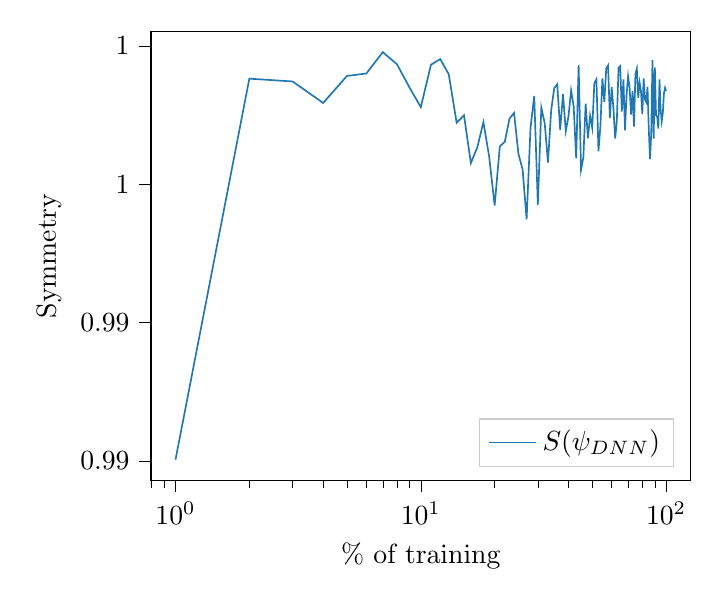
\begin{tikzpicture}

\definecolor{color0}{rgb}{0.12156862745098,0.466666666666667,0.705882352941177}

\begin{axis}[
legend cell align={left},
legend style={at={(0.97,0.03)}, anchor=south east, draw=white!80.0!black},
log basis x={10},
tick align=outside,
tick pos=left,
x grid style={white!69.01960784313725!black},
xlabel={\% of training},
xmin=0.794328234724281, xmax=125.892541179417,
xmode=log,
xtick style={color=black},
y grid style={white!69.01960784313725!black},
ylabel={Symmetry},
ymin=0.984309365052292, ymax=1.00050878754228,
ytick style={color=black}
]
\addplot [semithick, color0]
table {%
0 0.997930104443005
1 0.9850457024382
2 0.998813011878135
3 0.99871220252965
4 0.997935921623358
5 0.998911211393951
6 0.999000852677468
7 0.999772450156367
8 0.999329711279481
9 0.998490367941297
10 0.997783221653868
11 0.999315841618538
12 0.999519239876548
13 0.998975148737978
14 0.9972178954233
15 0.997489992887832
16 0.995764221941261
17 0.996333803020141
18 0.997243659373817
19 0.995997096454074
20 0.994227074110286
21 0.996364771987532
22 0.996531157045201
23 0.997372466342706
24 0.997574266841106
25 0.996101252312667
26 0.995533562607449
27 0.993730494773845
28 0.997020551968696
29 0.998192145115019
30 0.994257266631085
31 0.997763679217548
32 0.99721008060418
33 0.995779874849485
34 0.9976672680183
35 0.998471733748994
36 0.998609135808838
37 0.996966720235578
38 0.998252292292495
39 0.996917306280208
40 0.997449650489726
41 0.998389458028193
42 0.997812869080244
43 0.99593603022422
44 0.999304352431323
45 0.995516083524949
46 0.995971696646516
47 0.997911499990076
48 0.996656301335553
49 0.997473436229803
50 0.997033310558976
51 0.998647956314309
52 0.998789727421731
53 0.996190482945166
54 0.997124380357023
55 0.998822663882566
56 0.997974485563469
57 0.999175434971667
58 0.999291042905921
59 0.99739896499388
60 0.998501570053109
61 0.99773998730539
62 0.996647403876604
63 0.997323443502133
64 0.999211385013276
65 0.999271094667731
66 0.997627277468417
67 0.998785890411443
68 0.996950055073586
69 0.998228275481828
70 0.998897857323701
71 0.998495693536642
72 0.997518909785617
73 0.998363893038032
74 0.997079248759291
75 0.998984957310564
76 0.999175479769193
77 0.998118644714787
78 0.998667982463461
79 0.998371239471504
80 0.997529688518792
81 0.998823065540167
82 0.998066246198655
83 0.997967632020373
84 0.998513025096931
85 0.996997720894606
86 0.995904777124855
87 0.996845086569904
88 0.999481190035064
89 0.996645258283487
90 0.999215924958678
91 0.997490320916104
92 0.997436552691062
93 0.997012060696312
94 0.998786555000447
95 0.997689607752852
96 0.997274352109999
97 0.997580728741008
98 0.998282290358827
99 0.998480522217972
100 0.99836931859961
};
\addlegendentry{$S(\psi_{DNN})$}
\end{axis}

\end{tikzpicture}
%     }
%     \caption{\label{fig:QD-pade-dnn-symmetry}Permutation symmetry of
% $\psi_{DNN}$ as a function of training steps. See
% \cref{fig:QD-pade-dnn-training} for source code reference.}
% \end{figure}

\begin{figure}[h]
   \centering
    \resizebox{\linewidth}{!}{%
        % This file was created by matplotlib2tikz v0.7.4.
\begin{tikzpicture}

\begin{groupplot}[group style={group size=2 by 3}]
\nextgroupplot[
tick align=outside,
x grid style={white!69.01960784313725!black},
xmin=-0.5, xmax=31.5,
xtick pos=both,
xtick style={color=black},
y grid style={white!69.01960784313725!black},
ylabel={\(\displaystyle \mathbf{W}^{(0)}\)},
ymin=-0.5, ymax=3.5,
ytick pos=left,
ytick style={color=black}
]
\addplot graphics [includegraphics cmd=\pgfimage,xmin=-0.5, xmax=31.5, ymin=3.5, ymax=-0.5] {scripts/QD-pade-dnn.py.weights-000.png};

\nextgroupplot[
axis y line=right,
tick align=outside,
x grid style={white!69.01960784313725!black},
xmin=-0.5, xmax=31.5,
xtick pos=both,
xtick style={color=black},
y grid style={white!69.01960784313725!black},
ylabel={\(\displaystyle \mathbf{b}^{(0)}\)},
ymin=-0.5, ymax=0.5,
ytick pos=left,
ytick style={color=black},
ytick={-0.6,-0.4,-0.2,0,0.2,0.4,0.6},
yticklabels={−0.6,−0.4,−0.2,0.0,0.2,0.4,0.6}
]
\addplot graphics [includegraphics cmd=\pgfimage,xmin=-0.5, xmax=31.5, ymin=0.5, ymax=-0.5] {scripts/QD-pade-dnn.py.weights-001.png};

\nextgroupplot[
tick align=outside,
x grid style={white!69.01960784313725!black},
xmin=-0.5, xmax=15.5,
xtick pos=both,
xtick style={color=black},
y grid style={white!69.01960784313725!black},
ylabel={\(\displaystyle \mathbf{W}^{(1)}\)},
ymin=-0.5, ymax=31.5,
ytick pos=left,
ytick style={color=black}
]
\addplot graphics [includegraphics cmd=\pgfimage,xmin=-0.5, xmax=15.5, ymin=31.5, ymax=-0.5] {scripts/QD-pade-dnn.py.weights-002.png};

\nextgroupplot[
axis y line=right,
tick align=outside,
x grid style={white!69.01960784313725!black},
xmin=-0.5, xmax=15.5,
xtick pos=both,
xtick style={color=black},
y grid style={white!69.01960784313725!black},
ylabel={\(\displaystyle \mathbf{b}^{(1)}\)},
ymin=-0.5, ymax=0.5,
ytick pos=left,
ytick style={color=black},
ytick={-0.6,-0.4,-0.2,0,0.2,0.4,0.6},
yticklabels={−0.6,−0.4,−0.2,0.0,0.2,0.4,0.6}
]
\addplot graphics [includegraphics cmd=\pgfimage,xmin=-0.5, xmax=15.5, ymin=0.5, ymax=-0.5] {scripts/QD-pade-dnn.py.weights-003.png};

\nextgroupplot[
tick align=outside,
x grid style={white!69.01960784313725!black},
xlabel={Layer weights},
xmin=-0.5, xmax=0.5,
xtick pos=both,
xtick style={color=black},
xtick={-0.6,-0.4,-0.2,0,0.2,0.4,0.6},
xticklabels={−0.6,−0.4,−0.2,0.0,0.2,0.4,0.6},
y grid style={white!69.01960784313725!black},
ylabel={\(\displaystyle \mathbf{W}^{(2)}\)},
ymin=-0.5, ymax=15.5,
ytick pos=left,
ytick style={color=black}
]
\addplot graphics [includegraphics cmd=\pgfimage,xmin=-0.5, xmax=0.5, ymin=15.5, ymax=-0.5] {scripts/QD-pade-dnn.py.weights-004.png};

\nextgroupplot[
axis y line=right,
tick align=outside,
x grid style={white!69.01960784313725!black},
xlabel={Layer biases},
xmin=-0.5, xmax=0.5,
xtick pos=both,
xtick style={color=black},
xtick={-0.6,-0.4,-0.2,0,0.2,0.4,0.6},
xticklabels={−0.6,−0.4,−0.2,0.0,0.2,0.4,0.6},
y grid style={white!69.01960784313725!black},
ylabel={\(\displaystyle \mathbf{b}^{(2)}\)},
ymin=-0.5, ymax=0.5,
ytick pos=left,
ytick style={color=black},
ytick={-0.6,-0.4,-0.2,0,0.2,0.4,0.6},
yticklabels={−0.6,−0.4,−0.2,0.0,0.2,0.4,0.6}
]
\addplot graphics [includegraphics cmd=\pgfimage,xmin=-0.5, xmax=0.5, ymin=0.5, ymax=-0.5] {scripts/QD-pade-dnn.py.weights-005.png};
\end{groupplot}

\end{tikzpicture}
    }
    \caption[Weights of a neural network trained on quantum dots]{\label{fig:QD-pade-dnn-weights}Color map representation of the
weights and biases in the network of $\psi_{DNN}$. The left column of plots
shows the weight matrices in each layer, and the corresponding biases are in the
right column. The bottom right plot has only one color because there is only one
output layer bias. Each rectangle represents a parameter, and they have been
scaled to have the same total size. The size of the rectangles are not
important. See \cref{fig:QD-pade-dnn-training} for source code reference.}
\end{figure}

\subsection{Interpreting the Networks}

Given the apparent ability of the networks to improve upon our theoretically
motivated ansatz, it would be interesting to see if we can learn something from
the structure of the network. This is, however, notoriously difficult to do with
neural networks. In most cases the interconnections that make up the network are
simply treated as a black box, simply because we lack the understanding to do
anything else.

Still, we can make an attempt. \cref{fig:QD-pade-dnn-weights} show a color map
representation of all the weights and biases of $\psi_{DNN}$ after training.
Arguably, we should not attempt to assign physical meanings to any of the later
layers. If anything, the weight matrix of the first layer could be insightful,
as this is directly multiplied with the coordinates $\mat X$. Interestingly,
two columns appear to have significant values. This is very similar to the
effect seen in~\cref{fig:QD-rbm-symmetry} for the RBM. In fact, the same
symmetry between the two columns is even present. The remaining columns are not
as clearly zeroed out in the networks, perhaps due to the lack of
regularization. While non-trivial to interpret, this points to the networks
learning, completely by them selves, some underlying physical structure in the
inputs.



\subsection{Complexity}

While the neural network has demonstrated its capacity to learn an improved
correlation function, this does come at a considerable computational cost.

The benchmark function has complexity $\mathcal{O}(N^2)$ for $N$ particles,
rooted in the double sum in~\cref{eq:qd-pade-jastrow-anzats}. Thanks to
analytic expressions for the derivatives, the otherwise heavy Laplace operator
is also calculated in $\mathcal{O}(N^2)$ time.

The complexity of the neural network is a little harder to pin down, because of
the inherent flexibility in how the network can be structured.

The neural network computes a series of matrix-vector multiplications, both during
evaluation and for its derivatives. The input layer needs to scale equal to $N$,
while the other layers could in principle be constant. This means we could say
that the network only scales linearly, $\mathcal{O}(N)$, with increasing number
of particles. Still, the \say{constant} part of the computation time is very
large, and this kind of complexity analysis is slightly unfair.

In practice we found that we needed the second layer to have more
nodes than we have inputs. We have not determined a strict relationship, but
either $\mathcal{O}(N)$ or $\mathcal{O}{N^2}$ seems reasonable for the second
layer. Assuming the network shrinks from there on, the dominant operation is a
matrix-vector operation with matrix dimensions of order $(N\times N)$ or $(N\times N^2)$,
which works out to a complexity of $\mathcal{O}(N^2)$ or $\mathcal{O}(N^3)$. In
this more realistic view, the networks are not improving upon the complexity of
the benchmark, but rather the opposite is true.\\

Importantly the networks also depend highly on the depth (number of layers) as
well as obviously the sizes of subsequent layers. We should also note that while
asymptotic cost might be equal to the benchmark, a more precise count of the
required operations would show a substantial disparity.

However, a constant cost difference can always be brought down with optimized code, more
and better hardware, introducing \glspl{gpu} etc. And while computing power may no
longer increase exponentially each year, it continues to grow nevertheless.
Large scale use of networks for quantum mechanics might therefore be well
within reach.

\subsection{Other Observables}

So for we have only investigated the energies produced by the different wave
functions. Other observables of interest could be the mean distance from the origin,
$\expval{r}$, the mean squared distance from the origin, $\expval{r^2}$ and the mean
inter-particle distance, $\expval{r_{12}}$. These are all quantities that should
depend on the correlation between the particles.
\cref{tab:QD-mean-distance-metrics} shows the three observables as predicted
from the three wave functions trained previously.

\begin{table}[h]
  \centering
  \caption[Radial metrics of different wave functions on quantum dots]{Average distances predicted by the different wave functions. Results
    obtained by \gls{mci} using \gls{is} and $2^{24}$
    samples. The first row shows the corresponding values for a single particle
    in an ideal harmonic oscillator, with the values coming from the analytic
    expressions $\expval{r}=\flatfrac{\sqrt\pi}{2\sqrt\omega}$ and
    $\expval{r^2}=\omega^{-1}$. While the differences between $\psi_{PJ}$ and
    the networks are small, the inter-particle distance shows the largest
    difference. Distances in dimensionless units of $a_{ho}$.\citesource{writing/scripts/QD-other-metrics.py}}
  \begin{tabular}{l*3{S[table-format=3.6]}}
\toprule
\addlinespace
& {$\expval{r}$} & {$\expval{r^2}$} & {$\expval{r_{12}}$} \\
\addlinespace
\midrule
\addlinespace
\addlinespace
Ideal HO    & 0.88623 & 1.00000 & {---}\\
$\psi_{PJ}$ & 1.0192(2) & 1.2952(5) & 1.6337(5)\\
$\psi_{DNN}$  & 1.0197(2) & 1.2974(5) & 1.6393(5)\\
$\psi_{SDNN}$ & 1.0198(2) & 1.2964(5) & 1.6390(5)\\
\addlinespace\addlinespace\bottomrule
\end{tabular}
  \label{tab:QD-mean-distance-metrics}
\end{table}
We see first that, as one would expect, the predicted radii are larger when we
have multiple interacting particles. Less clear is the differences between the
benchmark wave function $\psi_{PJ}$ and the networks. In general, the results
indicate that $\psi_{PJ}$ slightly underestimates the effect of the Coulomb
repulsion. While $\expval{r}$ and $\expval{r^2}$ are not significantly different
from the networks, we see a larger difference in $\expval{r_{12}}$. This might
be because $\expval{r_{12}}$ is the quantity which is most directly
connected to the strength of the interaction

The two network types seem to once again be equivalent, with the observed differences well
within statistical expectations.

\end{document}
